% !Mode:: "TeX:UTF-8"

\def\usewhat{pdflatex}                               % 定义编译方式 dvipdfmx 或者 pdflatex,默认为 dvipdfmx
                                                     % 方式编译,如果需要修改,只需改变花括号中的内容即可。
\documentclass[12pt,openany,oneside,ctexartutf8]{book}
                                                     % 本科生毕业论文通常采用单页排版
% !Mode:: "TeX:UTF-8"
%  Authors: 张井   Jing Zhang: prayever@gmail.com     天津大学2010级管理与经济学部信息管理与信息系统专业硕士生
%           余蓝涛 Lantao Yu: lantaoyu1991@gmail.com  天津大学2008级精密仪器与光电子工程学院测控技术与仪器专业本科生

%%%%%%%%%% Package %%%%%%%%%%%%
\usepackage{graphicx}                       % 支持插图处理
% \usepackage[a4paper,text={146.4true mm,239.2 true mm},top= 25.4true mm, bottom= 25.4true mm, left=31.7 true mm,head=6true mm,headsep=6.5true mm,foot=16.5true mm]{geometry}
\usepackage[a4paper,top=25.4mm, bottom=25.4mm, left=31.7mm, right=31.7mm, head=6true mm,headsep=6.5true mm,foot=17.5mm]{geometry}
                                            % 支持版面尺寸设置
\usepackage[squaren]{SIunits}               % 支持国际标准单位

\usepackage{titlesec}                       % 控制标题的宏包
\usepackage{titletoc}                       % 控制目录的宏包
\usepackage{fancyhdr}                       % fancyhdr宏包 支持页眉和页脚的相关定义
\usepackage[UTF8, fontset=windows]{ctex}                    % 支持中文显示
\usepackage{CJKpunct}
\usepackage{color}                          % 支持彩色
\usepackage{amsmath}                        % AMSLaTeX宏包 用来排出更加漂亮的公式
\usepackage{amssymb}                        % 数学符号生成命令
\usepackage[below]{placeins}    %允许上一个section的浮动图形出现在下一个section的开始部分,还提供\FloatBarrier命令,使所有未处理的浮动图形立即被处理
\usepackage{multirow}                       % 使用Multirow宏包,使得表格可以合并多个row格
\usepackage{booktabs}                       % 表格,横的粗线;\specialrule{1pt}{0pt}{0pt}
\usepackage{longtable}                      % 支持跨页的表格。
\usepackage{tabularx}                       % 自动设置表格的列宽
\usepackage{subfigure}                      % 支持子图 %centerlast 设置最后一行是否居中
\usepackage[subfigure]{ccaption}            % 支持子图的中文标题
\usepackage[sort&compress,numbers]{natbib}  % 支持引用缩写的宏包
\usepackage{enumitem}                       % 使用enumitem宏包,改变列表项的格式
\usepackage{calc}                           % 长度可以用+ - * / 进行计算
\usepackage{txfonts}                        % 字体宏包
\usepackage{bm}                             % 处理数学公式中的黑斜体的宏包
\usepackage[amsmath,thmmarks,hyperref]{ntheorem}  % 定理类环境宏包,其中 amsmath 选项用来兼容 AMS LaTeX 的宏包
\usepackage{CJKnumb}                        % 提供将阿拉伯数字转换成中文数字的命令
\usepackage{indentfirst}                    % 首行缩进宏包
\usepackage{CJKutf8}                        % 用在UTF8编码环境下,它可以自动调用CJK,同时针对UTF8编码作了设置

% \usepackage{fancybox} 

%\usepackage{hypbmsec}                      % 用来控制书签中标题显示内容
\newcommand{\tabincell}[2]{\begin{tabular}{@{}#1@{}}#2\end{tabular}}
\usepackage{xcolor}
%支持代码环境
\usepackage{listings}
\lstset{numbers=left,
language=[ANSI]{C},
numberstyle=\tiny,
extendedchars=false,
showstringspaces=false,
breakatwhitespace=false,
breaklines=true,
captionpos=b,
keywordstyle=\color{blue!70},
commentstyle=\color{red!50!green!50!blue!50},
frame=shadowbox,
rulesepcolor=\color{red!20!green!20!blue!20}
}
%支持算法环境
\usepackage[boxed,ruled,lined]{algorithm2e}
\usepackage{algorithmic}

\usepackage{array}
\newcommand{\PreserveBackslash}[1]{\let\temp=\\#1\let\\=\temp}
\newcolumntype{C}[1]{>{\PreserveBackslash\centering}p{#1}}
\newcolumntype{R}[1]{>{\PreserveBackslash\raggedleft}p{#1}}
\newcolumntype{L}[1]{>{\PreserveBackslash\raggedright}p{#1}}

% 生成有书签的 pdf 及其生成方式。通常可以在 tjumain.tex 文件的第一行选择 pdflatex 或者是 dvipdfmx 编译手段。如果选择前者,则使用 pdflatex + pdflatex 编译; 如果选择后者,在编译的时候选择 latex + bibtex + latex + latex 编译。出现混淆的时候,系统会报错。
% 如果您的pdf制作中文书签有乱码使用如下命令,就可以解决了
\def\atemp{pdflatex}\ifx\atemp\usewhat
\usepackage{cmap}                           % pdflatex 编译时,可以生成可复制、粘贴的中文 PDF 文档, 缺点是在Windows上显示时效果不大好,字体发虚
\usepackage{hyperref}
\hypersetup{
    unicode,
    pdfborder={0 0 0},
}
\fi
% \usepackage[pdftex,unicode,
%             CJKbookmarks=true,
%             bookmarksnumbered=true,
%             bookmarksopen=true,
%             colorlinks=false,
%             pdfborder={0 0 0},
%             citecolor=blue,
%             linkcolor=red,
%             anchorcolor=green,
%             urlcolor=blue,
%             breaklinks=true
%             ]{hyperref}

                                % 定义本文所使用宏包
\graphicspath{{figures/}}                            % 定义所有的 .eps 文件在 figures 子目录下
\begin{document}                                     % 开始全文
\begin{CJK*}{UTF8}{song}                             % 开始中文字体使用
	% !Mode:: "TeX:UTF-8"
%  Authors: 张井   Jing Zhang: prayever@gmail.com     天津大学2010级管理与经济学部信息管理与信息系统专业硕士生
%           余蓝涛 Lantao Yu: lantaoyu1991@gmail.com  天津大学2008级精密仪器与光电子工程学院测控技术与仪器专业本科生

% 2018/5/23修正
%           李幼萌 Youmeng Li: liyoumeng@tju.edu.cn   天津大学软件学院软件工程系

%%%%%%%%%%%%%%%%% Fonts Definition and Basics %%%%%%%%%%%%%%%%%
\newcommand{\song}{\CJKfamily{song}}    % 宋体
\newcommand{\fs}{\CJKfamily{fs}}        % 仿宋体
\newcommand{\kai}{\CJKfamily{kai}}      % 楷体
\newcommand{\hei}{\CJKfamily{hei}}      % 黑体
\newcommand{\li}{\CJKfamily{li}}        % 隶书
\newcommand{\yihao}{\fontsize{26pt}{26pt}\selectfont}       % 一号, 单倍行距
\newcommand{\xiaoyi}{\fontsize{24pt}{24pt}\selectfont}      % 小一, 单倍行距
\newcommand{\erhao}{\fontsize{22pt}{1.25\baselineskip}\selectfont}       % 二号, 1.25倍行距
\newcommand{\xiaoer}{\fontsize{18pt}{18pt}\selectfont}      % 小二, 单倍行距
\newcommand{\sanhao}{\fontsize{16pt}{16pt}\selectfont}      % 三号, 单倍行距
\newcommand{\xiaosan}{\fontsize{15pt}{15pt}\selectfont}     % 小三, 单倍行距
\newcommand{\sihao}{\fontsize{14pt}{14pt}\selectfont}       % 四号, 单倍行距
\newcommand{\xiaosi}{\fontsize{12pt}{12pt}\selectfont}      % 小四, 单倍行距
\newcommand{\wuhao}{\fontsize{10.5pt}{10.5pt}\selectfont}   % 五号, 单倍行距
\newcommand{\xiaowu}{\fontsize{9pt}{9pt}\selectfont}        % 小五, 单倍行距

\CJKtilde  % 重新定义了波浪符~的意义
\newcommand\prechaptername{第}
\newcommand\postchaptername{章}

\punctstyle{hangmobanjiao}             % 调整中文字符的表示,行内占一个字符宽度,行尾占半个字符宽度

% 调整罗列环境的布局
\setitemize{leftmargin=3em,itemsep=0em,partopsep=0em,parsep=0em,topsep=-0em}
\setenumerate{leftmargin=3em,itemsep=0em,partopsep=0em,parsep=0em,topsep=0em}

% 避免宏包 hyperref 和 arydshln 不兼容带来的目录链接失效的问题。
\def\temp{\relax}
\let\temp\addcontentsline
\gdef\addcontentsline{\phantomsection\temp}

% 自定义项目列表标签及格式 \begin{publist} 列表项 \end{publist}
\newcounter{pubctr} %自定义新计数器
\newenvironment{publist}{%%%%%定义新环境
\begin{list}{[\arabic{pubctr}]} %%标签格式
    {
     \usecounter{pubctr}
     \setlength{\leftmargin}{2.5em}   % 左边界 \leftmargin =\itemindent + \labelwidth + \labelsep
     \setlength{\itemindent}{0em}     % 标号缩进量
     \setlength{\labelsep}{1em}       % 标号和列表项之间的距离,默认0.5em
     \setlength{\rightmargin}{0em}    % 右边界
     \setlength{\topsep}{0ex}         % 列表到上下文的垂直距离
     \setlength{\parsep}{0ex}         % 段落间距
     \setlength{\itemsep}{0ex}        % 标签间距
     \setlength{\listparindent}{0pt}  % 段落缩进量
    }}
{\end{list}}

\makeatletter
\renewcommand\normalsize{
  \@setfontsize\normalsize{12pt}{12pt} % 小四对应 12 pt
  \setlength\abovedisplayskip{4pt}
  \setlength\abovedisplayshortskip{4pt}
  \setlength\belowdisplayskip{\abovedisplayskip}
  \setlength\belowdisplayshortskip{\abovedisplayshortskip}
  \let\@listi\@listI}
\def\defaultfont{\renewcommand{\baselinestretch}{1.63}\normalsize\selectfont} % 设置行距

\renewcommand{\CJKglue}{\hskip -0.1 pt plus 0.08\baselineskip} % 控制字间距,使每行 34 个汉字
\makeatother

%%%%%%%%%%%%% Contents %%%%%%%%%%%%%%%%%
\renewcommand{\contentsname}{目\qquad 录}
\setcounter{tocdepth}{1} % 控制目录深度
\titlecontents{chapter}[2em]{\vspace{.5\baselineskip}\xiaosan\song}
             {\prechaptername\CJKnumber{\thecontentslabel}\postchaptername\qquad}{}
             {\hspace{.5em}\titlerule*[10pt]{$\cdot$}\sihao\contentspage}
\titlecontents{section}[4.2em]{\vspace{.25\baselineskip}\sihao\song}
             {\thecontentslabel\quad}{}
             {\hspace{.5em}\titlerule*[10pt]{$\cdot$}\sihao\contentspage}
% \titlecontents{subsection}[4em]{\vspace{.25\baselineskip}\xiaosi\song}
%              {\thecontentslabel\quad}{}
%              {\hspace{.5em}\titlerule*[10pt]{$\cdot$}\sihao\contentspage}

%%%%%%%%%% Chapter and Section %%%%%%%%%%%%%
\setcounter{secnumdepth}{4}
\setlength{\parindent}{2em}

\renewcommand{\chaptername}{\prechaptername\CJKnumber{\thechapter}\postchaptername}
\titleformat{\chapter}{\centering}{\xiaosan\song}{\chaptername}{} %{2em}
\titlespacing{\chapter}{0pt}{0.1\baselineskip}{0.8\baselineskip}

\titleformat{\section}{\sihao\hei}{\thesection}{1em}{}
\titlespacing{\section}{0pt}{0.15\baselineskip}{0.25\baselineskip}

\titleformat{\subsection}{\sihao\hei}{\thesubsection}{1em}{}
\titlespacing{\subsection}{0pt}{0.1\baselineskip}{0.3\baselineskip}

\titleformat{\subsubsection}{\sihao\hei}{\thesubsubsection}{1em}{}
\titlespacing{\subsubsection}{0pt}{0.05\baselineskip}{0.1\baselineskip}

%%%%%%%%%% Table, Figure and Equation %%%%%%%%%%%%%%%%%
\renewcommand{\tablename}{表}                                     % 插表题头
\renewcommand{\figurename}{图}                                    % 插图题头
\renewcommand{\thefigure}{\arabic{chapter}-\arabic{figure}}       % 使图编号为 7-1 的格式 %\protect{~}
\renewcommand{\thesubfigure}{\alph{subfigure})}                   % 使子图编号为 a) 的格式
\renewcommand{\thesubtable}{(\alph{subtable})}                    % 使子表编号为 (a) 的格式
\renewcommand{\thetable}{\arabic{chapter}-\arabic{table}}         % 使表编号为 7-1 的格式
\renewcommand{\theequation}{\arabic{chapter}-\arabic{equation}}   % 使公式编号为 7-1 的格式

%%%%%% 定制浮动图形和表格标题样式 %%%%%%
\makeatletter
\long\def\@makecaption#1#2{
   \vskip\abovecaptionskip
   \sbox\@tempboxa{\centering\wuhao\song{#1\qquad #2} }
   \ifdim \wd\@tempboxa >\hsize
     \centering\wuhao\song{#1\qquad #2} \par
   \else
     \global \@minipagefalse
     \hb@xt@\hsize{\hfil\box\@tempboxa\hfil}
   \fi
   \vskip\belowcaptionskip}
\makeatother
\captiondelim{~~~~} %用来控制longtable表头分隔符

%%%%%%%%%% Theorem Environment %%%%%%%%%%%%%%%%%
\theoremstyle{plain}
\theorembodyfont{\song\rmfamily}
\theoremheaderfont{\hei\rmfamily}
\newtheorem{theorem}{定理~}[chapter]
\newtheorem{lemma}{引理~}[chapter]
\newtheorem{axiom}{公理~}[chapter]
\newtheorem{proposition}{命题~}[chapter]
\newtheorem{prop}{性质~}[chapter]
\newtheorem{corollary}{推论~}[chapter]
\newtheorem{definition}{定义~}[chapter]
\newtheorem{conjecture}{猜想~}[chapter]
\newtheorem{example}{例~}[chapter]
\newtheorem{remark}{注~}[chapter]
%\newtheorem{algorithm}{算法~}[chapter]
\newenvironment{proof}{\noindent{\hei 证明:}}{\hfill $ \square $ \vskip 4mm}
\theoremsymbol{$\square$}

%%%%%%%%%% Page: number, header and footer  %%%%%%%%%%%%%%%%%

%\frontmatter 或 \pagenumbering{roman}
%\mainmatter 或 \pagenumbering{arabic}
\makeatletter
\renewcommand\frontmatter{\clearpage
  \@mainmatterfalse
  }
\makeatother

%%%%%%%%%%%% References %%%%%%%%%%%%%%%%%
\renewcommand{\bibname}{参考文献}
% 重定义参考文献样式,来自thu
\makeatletter
\renewenvironment{thebibliography}[1]{
    \titleformat{\chapter}{\raggedright\sihao\hei}{\chaptername}{2em}{}
   \chapter*{\bibname}
   \wuhao
   \list{\@biblabel{\@arabic\c@enumiv}}
        {\renewcommand{\makelabel}[1]{##1\hfill}
         \settowidth\labelwidth{0 cm}
         \setlength{\labelsep}{0pt}
         \setlength{\itemindent}{0pt}
         \setlength{\leftmargin}{\labelwidth+\labelsep}
         \addtolength{\itemsep}{-0.7em}
         \usecounter{enumiv}
         \let\p@enumiv\@empty
         \renewcommand\theenumiv{\@arabic\c@enumiv}}
    \sloppy\frenchspacing
    \clubpenalty4000
    \@clubpenalty \clubpenalty
    \widowpenalty4000
    \interlinepenalty4000
    \sfcode`\.\@m}
   {\def\@noitemerr
     {\@latex@warning{Empty `thebibliography' environment}}
    \endlist\frenchspacing}
\makeatother

\addtolength{\bibsep}{-0.5em}     % 缩小参考文献间的垂直间距
\setlength{\bibhang}{2em}         % 每个条目自第二行起缩进的距离

% 参考文献引用作为上标出现
%\newcommand{\citeup}[1]{\textsuperscript{\cite{#1}}}
\makeatletter
    \def\@cite#1#2{\textsuperscript{[{#1\if@tempswa , #2\fi}]}}
\makeatother
%% 引用格式
\bibpunct{[}{]}{,}{s}{}{,}

%%%%%%%%%%%% Cover %%%%%%%%%%%%%%%%%
% 封面、摘要、版权、致谢格式定义
\makeatletter
\def\ctitle#1{\def\@ctitle{#1}}\def\@ctitle{}
\def\cdegree#1{\def\@cdegree{#1}}\def\@cdegree{}
\def\caffil#1{\def\@caffil{#1}}\def\@caffil{}
\def\csubject#1{\def\@csubject{#1}}\def\@csubject{}
\def\cgrade#1{\def\@cgrade{#1}}\def\@cgrade{}
\def\cauthor#1{\def\@cauthor{#1}}\def\@cauthor{}
\def\cnumber#1{\def\@cnumber{#1}}\def\@cnumber{}
\def\cstuid#1{\def\@cstuid{#1}}\def\@cstuid{}
\def\cdate#1{\def\@cdate{#1}}\def\@cdate{}
\long\def\cabstract#1{\long\def\@cabstract{#1}}\long\def\@cabstract{}
\long\def\eabstract#1{\long\def\@eabstract{#1}}\long\def\@eabstract{}
\def\ckeywords#1{\def\@ckeywords{#1}}\def\@ckeywords{}
\def\ekeywords#1{\def\@ekeywords{#1}}\def\@ekeywords{}
\def\cheading#1{\def\@cheading{#1}}\def\@cheading{}
\def\ccovertitle#1{\def\@ccovertitle{#1}}\def\@ccovertitle{}

\pagestyle{fancy}
  \fancyhf{}
  \fancyhead[C]{\song\wuhao \@cheading}  % 页眉显示天津大学 20XX 届本科生毕业论文
  \fancyfoot[C]{\song\xiaowu ~\thepage~}
\newlength{\@title@width}

% 定义封面
\def\makecover{
%\cleardoublepage%
   \phantomsection
    \pdfbookmark[-1]{\@ctitle}{ctitle}

    \begin{titlepage}
      \vspace*{10pt}
      \begin{center}

      \begin{figure}[h]
      \centering
      
\includegraphics[width=0.4\textwidth]{figures/tju}
      \end{figure}
      \vspace*{15pt}
      \hei\erhao{\textbf{\@ccovertitle}} \\
      \hei\erhao{\textbf{\@ctitle}}
      \vspace*{55pt}

      \begin{figure}[h]
      \centering
      
\includegraphics[width=0.3\textwidth]{figures/Tjulogo}
      \end{figure}

      \vspace*{60pt}
      \renewcommand\arraystretch{1.5}
      \setlength{\@title@width}{5cm}
      {
        \sanhao\song{
          \begin{tabular}{lc}
            \textbf{学\qquad 院}  &  \underline{\makebox[\@title@width][c]{\textbf{\@caffil}}} \\
            \textbf{专\qquad 业}  &  \underline{\makebox[\@title@width][c]{\textbf{\@csubject}}} \\
            \textbf{年\qquad 级}  &  \underline{\makebox[\@title@width][c]{\textbf{\@cgrade}}}\\
            % \textbf{姓\qquad 名}  &  \underline{\makebox[\@title@width][c]{\textbf{\@cauthor}}}\\
            % \textbf{学\qquad 号}  &  \underline{\makebox[\@title@width][c]{\textbf{\@cstuid}}}\\
          \end{tabular}
        }
    }
    \vspace*{40pt}

    \song\sanhao{\textbf{\@cdate}}
    \end{center}
    \end{titlepage}
}

                             % 完成对论文各个部分格式的设置
	% !Mode:: "TeX:UTF-8"


%%%%%%%%%%%%%%%%%%%%%%%%%%%%%%%%%%%%%%%%%%%%%%%%%%%%%%%%%%%%%%%
%%  可通过对 setup/format.tex中                               %%
%%  第243行 \setlength{\@title@width}{5cm}中 5cm 这个参数来   %%
%%  控制封面中下划线的长度。                                   %%
%%%%%%%%%%%%%%%%%%%%%%%%%%%%%%%%%%%%%%%%%%%%%%%%%%%%%%%%%%%%%%

\cheading{天津大学 高级实践~\the\year~年 UkraineBHelper~需求规格说明书}      % 正文页眉
\ccovertitle{《高级实践》需求报告}                       % 封面标题

%%%%%%%%%%%%%%%%%%%%%%%%%%%%%%%%%%%%%%%%%%%%%%%%%%%%%%%%%%%%%
%%%%%%%%%% 以下为论文的基本信息,需要由作者进行修改 %%%%%%%%%%%%
%%%%%%%%%%%%%%%%%%%%%%%%%%%%%%%%%%%%%%%%%%%%%%%%%%%%%%%%%%%%%
\ctitle{UkraineBHelper~需求规格说明书 \\ 文档编号:DOC-RM-220329}    % 封面用论文标题,自己可手动断行
\caffil{软件学院}       % 学院名称
\csubject{软件工程}     % 专业名称
\cgrade{2019}           % 年级
% \cauthor{姓名}          % 学生姓名
% \cstuid{1234567890}     % 学号

\cdate{\the\year~年~\the\month~月~\the\day~日}  % 论文完成日期,不需要修改,自动生成

	\frontmatter                                     % 以下是论文导言部分,包括论文的封面,中英文摘要和中文目录
	\fancypagestyle{plain}{							 % 正文前均无页眉
		\fancyhf{}
		\renewcommand{\headrulewidth}{0 pt}
		\fancyfoot[C]{\song\xiaowu~\thepage~}
	}

	\makecover 			% 封面

	% !Mode:: "TeX:UTF-8"

% 目录
\defaultfont
\clearpage{
    \pagestyle{empty}
    \cleardoublepage
    \setcounter{page}{1}                                 % 单独从 1 开始编页码
    \pagenumbering{arabic}
    \titleformat{\chapter}{\centering\sanhao\hei}{\chaptername}{2em}{} % 设置目录两字的格式
    \pdfbookmark[0]{目~~录}{mulu}
    \tableofcontents                                     % 中文目录
    \thispagestyle{plain}
} % 目录

	\mainmatter\defaultfont\sloppy\raggedbottom
	\makeatletter
	\fancypagestyle{plain}{                              % 设置正文眉页脚风格
		\fancyhf{}
		\fancyhead[C]{\song\wuhao \@cheading}            % 页眉格式
		\fancyfoot[C]{\song\xiaowu ~\thepage~}           % 页脚格式
		\renewcommand{\headrulewidth}{0.5pt}
		\renewcommand{\footrulewidth}{0pt}
	}
	\makeatother
	\setcounter{page}{1}                                 % 单独从 1 开始编页码
	\titleformat{\chapter}{\centering\xiaosan\hei}{\chaptername}{2em}{} % 恢复chapter标题格式要求

	%%%%%% 这里是正文,每个文件对应正文中的一章 %%%%%%

	\chapter{简介}

战争冲突中,受伤的总是民众。本项目旨在从人道主义出发,搭建帮助难民的互助救助系统。本次主要关注的是俄乌冲突中的受伤民众,他们的安危是俄乌两国在谈判中的议题之一,也收到了国际社会的关注。
\\
\section{背景}

战争的出现是大国之间的博弈和多方利益的考量,在战争中民众的生命安全一直是参战双方的谈判议题,以近期出现的俄乌冲突为例,早在俄乌之间的战争还未爆发的前一周,乌克兰的前一百名富豪们就有96名乘包机逃离了乌克兰,在战时状态,剩下的乌克兰老百姓不仅不被允许离境,还发放枪支给他们,希望他们抵抗。甚至连部分女性,也被迫成为士兵,派往战场。这些人中,很多人都是在两天的时间内才学会射击。

一个逃难去到波兰的乌克兰难民小男孩在被问道,为什么不去选一件为难民孩子们捐赠的玩具,反而一个人在这里孤独悲伤地坐着?他回答说:“小男孩?我现在是家里的大人了”。

在冲突的民众,主要面临以下问题:

\begin{itemize}
\item 缺少食物,淡水,住所等基本生存需求。
\item 缺少基本应急药品。
\item 与临近国家语言不通。
\item 无法与家人团聚 。
\end{itemize}

解决这些问题也是我们开发设计这套系统首要关注的内容。
\\
\section{定义、缩略语}

\begin{table}[htbp]
  \centering
  \caption{定义、缩略语}
  \vspace{0.5em}\wuhao
  \begin{tabular}{|c|c|}
    \hline
    \makebox[0.2\textwidth][c]{术语} & \makebox[0.2\textwidth][c]{解释}   \\
    \hline
    无                               & 无                                \\
    \hline
  \end{tabular}
\end{table}

\section{约束}

\begin{itemize}
  \item 相关需要有身份认证以保证安全性。
  \item 系统无前置的软硬件基础。
\end{itemize}
\newpage
\section{参考资料}
\begin{table}[htbp]
  \centering
  \caption{参考资料 }
  \vspace{0.5em}\wuhao
  \begin{tabular}{|c|c|c|c|c|}
    \hline
    \makebox[0.2\textwidth][c]{资料名称} & \makebox[0.2\textwidth][c]{版本日期} & \makebox[0.2\textwidth][c]{说明} \\
    \hline
    UML大战需求分析                      & 2012年2月第一版                      & 无                               \\
    \hline
    待补充                               &                                      &                                  \\
    \hline
  \end{tabular}
\end{table}


\chapter{架构设计}

\section{总体架构}
该系统采用的是微服务架构,即将业务拆分为多个子业务独立部署,各个子业务之间彼此独立,互相协作。同时整合网关、注册中心、负载均衡等当下流行的微服务技术,
使得各个服务之间的协作更加有合理、高效。同时为了应对集群部署,也为了提高处理速度,本系统采用Redis缓存技术,以便部分业务的处理。总体的架构图如图~\ref{fig:framework}~所示。
\begin{figure}[htbp]
    \centering
    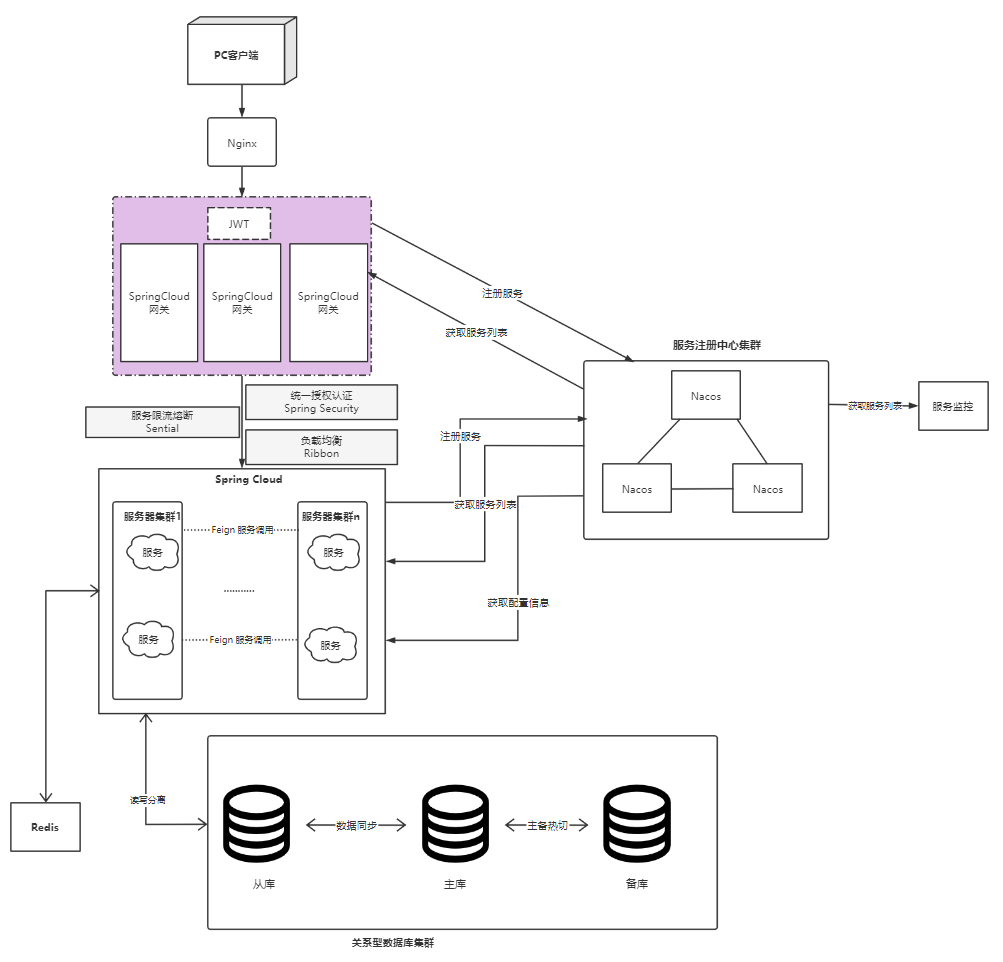
\includegraphics[width=\textwidth]{ch2/framework.png}
    \caption{总体架构}\label{fig:framework}
    \vspace{\baselineskip} % 表示图与正文空一行
\end{figure}

\subsection{具体微服务模块}
具体的微服务模块即系统给用户提供的业务服务,包括注册认证、发帖浏览等,每个具体微服务都整合了SpringCloud框架,微服务之间通过OpenFeign进行相互调用。
各个微服务集群部署,负载均衡技术采用ribbon,负载均衡策略为轮询。

\subsection{中间件}
本系统采用了许多微服务的中间件,以便更好地为微服务框架服务。
\subsubsection{服务注册与发现}
服务注册采用的是阿里巴巴开发的Nacos,部署方法为3个Nacos搭建服务注册集群。该集群可以实现各个微服务的注册,服务列表的获取和微服务的监听。
\subsubsection{服务调用}
本系统的服务调用技术采用的是OpenFeign,其为HTTP形式的REST API提供了简洁高效的RPC调用方式,同时OpenFeign也整合了负载均衡功能,便于集群之间的调用。
\subsubsection{负载均衡}
负载均衡技术使用的是Ribbon,结合OpenFeign实现微服务集群之间的互相调用,鉴于本系统的流量并不大,因此负载均衡策略采用轮询即可。
\subsubsection{网关}
网关技术使用的是Spring Gateway,他为众多服务模块提供了一个统一的访问路径,同时负责分发路由和认证授权,是所有服务调用的第一步。
\subsubsection{配置中心}
配置中心使用Nacos的配置中心,和Nacos服务注册中心紧密结合,将项目的配置文件进行统一的管理,同时也将项目的开发环境进行有效的隔离。
\subsubsection{服务降级和服务熔断}
本系统采用Sentinel技术实现服务降级和服务熔断,在流量超出服务器上限,或是出错率超过阈值时,会返回特定页面,以给客户更好的服务体验。
\subsubsection{消息队列}
本系统采用RabbitMQ实现消息队列,实现应用之间的异步调用,使得一些不需要及时反馈的操作可以异步进行,从而加快响应速度,提高用户体验。


\subsection{存储与缓存}
\subsubsection{数据库}
系统采用的为MySQL数据库,其数据模型的具体请详见后面的详细设计,会将每张数据表的字段和约束具体描述。
\subsubsection{缓存}
系统采用的是Redis缓存,其是基于内存的非关系型数据库,用于为本系统提升查询速度,主要在认证授权模块等高频模块使用。



\chapter{高层设计}
通过全局,虽然我们对该系统采用的是微服务架构,但是纵向来说,对于某个具体的模块,我们依然采用传统的MVC模式,即区分视图层、业务层和持久层。
视图层负责和前端进行数据交互,业务层负责业务逻辑处理,持久层负责和数据库进行数据交互,三层各司其职,实现系统的可控、可扩展。本章针对需求规格说明书提出
的需求进行提炼,给出本系统的层次结构,包括包图、部署图等设计。

\section{模块图}
系统中我们分为了许多Modules,主要为4个模块,Common、Service、GateWay、NacosCore,其作用分别是通用工具模块,微服务业务模块,网管模块和服务注册中心模块,
下面图~\ref{fig:Modules}~给出了系统的总体模块图。
\begin{figure}[htbp]
    \centering
    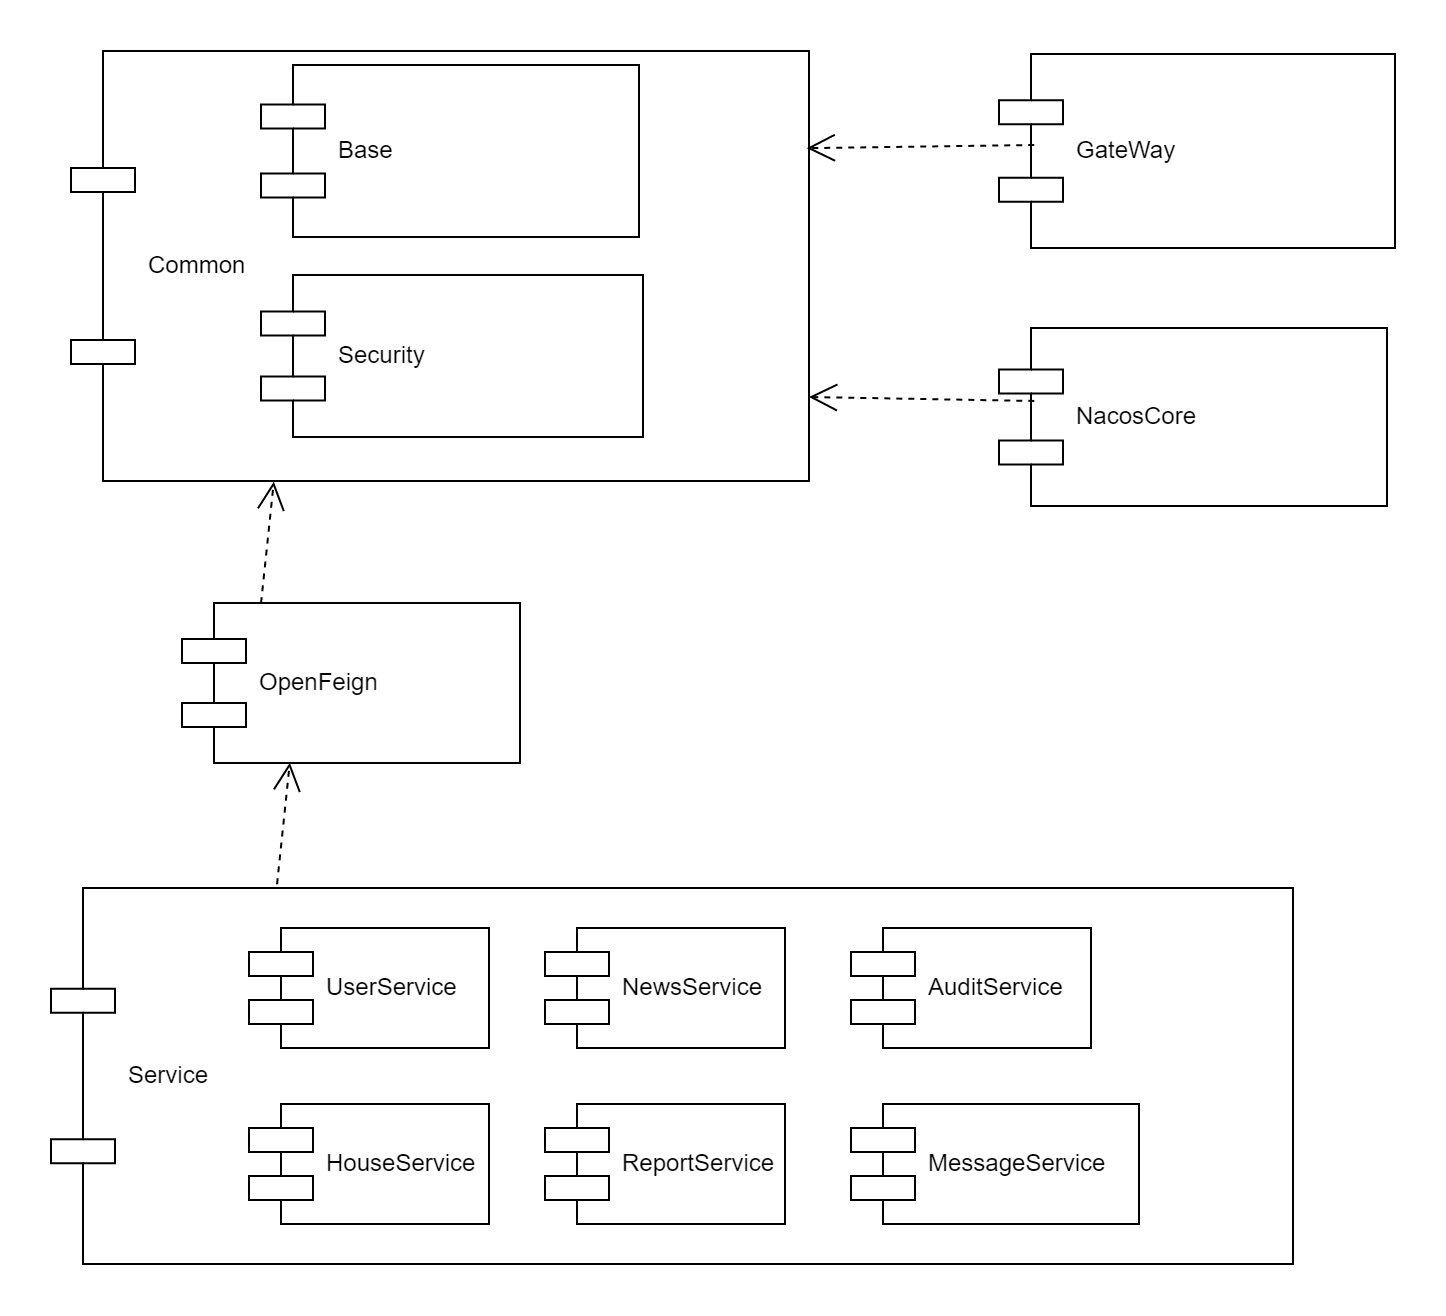
\includegraphics[width=\textwidth]{ch3/Modules.jpg}
    \caption{模块图}\label{fig:Modules}
    \vspace{\baselineskip} % 表示图与正文空一行
\end{figure}

其中四个模块还含有不同的子模块,我们对于四个模块的作用及其子模块做一个大致说明。
\begin{itemize}
    \item Common通用工具模块,将其他模块通用的功能抽象成一个独立的模块,便于调用。
    \begin{itemize}
        \item Base模块,包含了一些基本配置,比如Redis缓存的配置,返回类的配置等等。
        \item Security模块,整合了SpringSecurity框架,用于对用户进行认证授权。
    \end{itemize}
    \item Service微服务业务模块,即负责系统实际业务的模块,将所有业务统一到一个父类模块下,便于统一配置。
    \begin{itemize}
        \item UserService模块,负责处理用户信息的模块,包括用户登录、用户注册、管理获取用户列表等。
        \item HouseService模块,负责处理房源帖子的信息,包括发帖、改贴、帖子列表等。
        \item ReportService模块,负责举报信息,包括发起举报,审核举报等。
        \item NewsService模块,负责管理新闻信息,包括编辑新闻,获取新闻列表等。
        \item AuditService模块,负责管理审核信息,包括举报审核、新闻审核等。
        \item SystemService模块,负责处理系统的消息和系统业务对象,用于管理员给用户群发通知,业务对象管理等。
    \end{itemize}
    \item GateWay网管模块,负责分发路由,将请求转发到对应的微服务上,同时也负责初步校验JWT,检验用户身份。
    \item NacosCore微服务注册中心模块,负责管理系统中的各项微服务,包括服务注册、服务发现、流量监控等。
\end{itemize}

\section{包图}
接下来我们来设计各个模块中的包结构,不同功能的模块有着不同的包结构。大体来说,业务模块主要以MVC模式为主,即不同的层次对应不同的包,而配置相关的模块则
会根据配置类别进行不同的分包。

\subsection{Common通用工具模块}
Common模块中包含两个子模块,为Base模块和Security模块。
\subsubsection{Base}
Base中主要包含两个包,分别是Config和Util,分别负责一些全局参数的配置。Config中包含了Redis、RestTemplate、Constant(全局常量)的配置。Util中包含了ResponseUtil(统一返回设置)、Result(统一返回类)等全局统一用的配置。
Base模块的总体包图如图~\ref{fig:Base}~所示。
\begin{figure}[htbp]
    \centering
    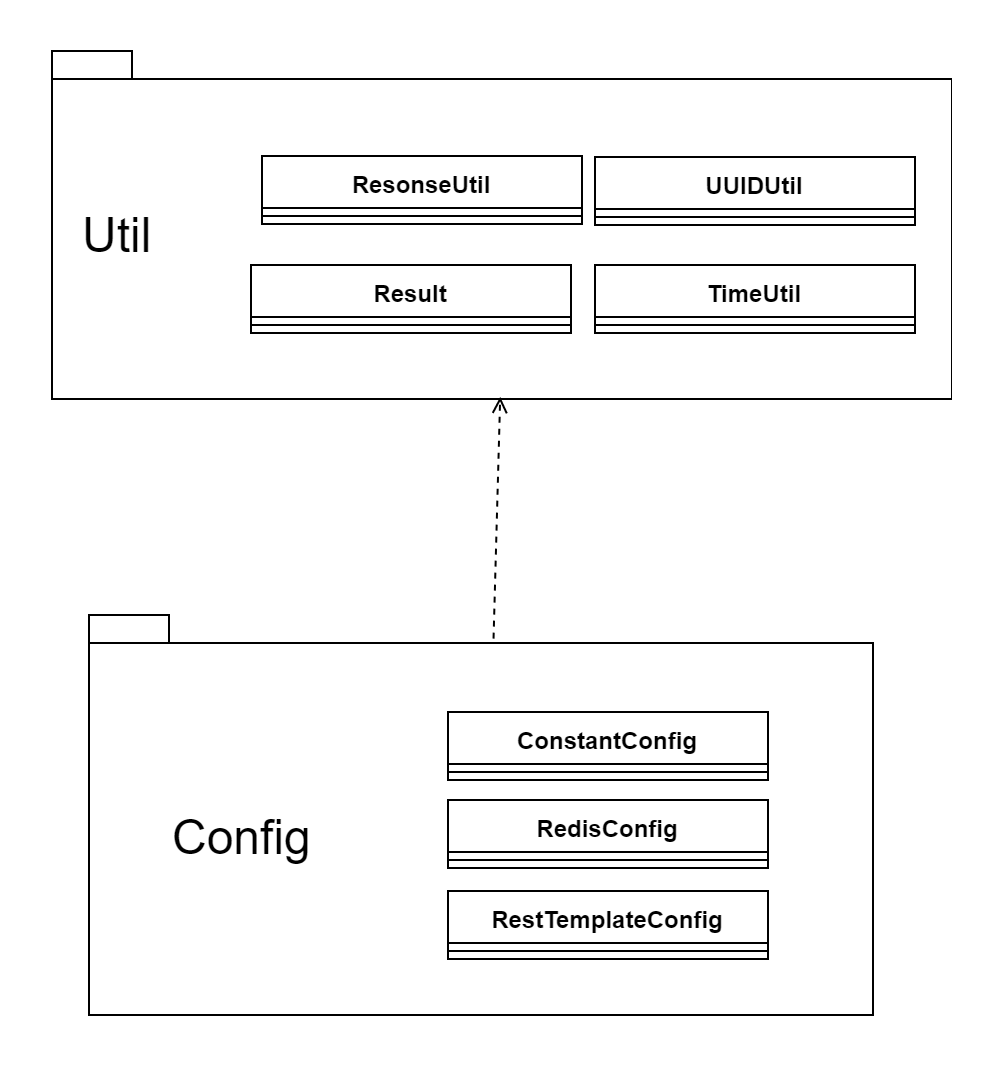
\includegraphics[width=0.6\textwidth]{ch3/Base.jpg}
    \caption{Base模块包图}\label{fig:Base}
    \vspace{\baselineskip} % 表示图与正文空一行
\end{figure}

\subsubsection{Security}
Security中主要包含4个包,为Config、Filter、Entity、Security。其中,Config为安全框架的具体配置,Filter中自定了一些过滤器,Entity中定义了一些实体类,Security中定义了具体的认证授权操作类。
Security模块的总体包图如图~\ref{fig:Security}~所示。
\begin{figure}[htbp]
    \centering
    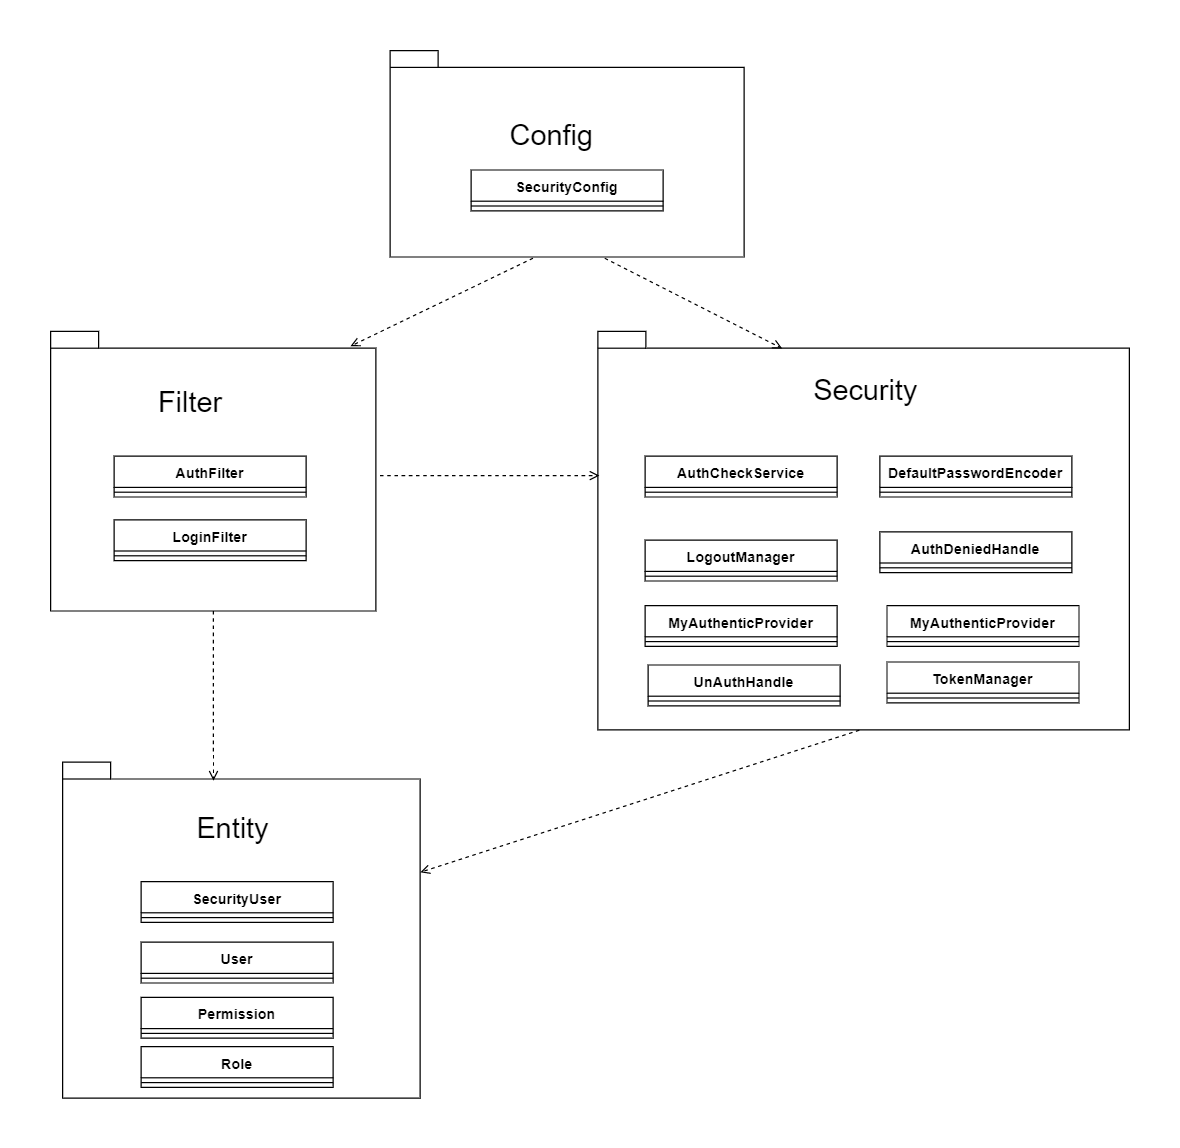
\includegraphics[width=\textwidth]{ch3/Security.jpg}
    \caption{Security模块包图}\label{fig:Security}
    \vspace{\baselineskip} % 表示图与正文空一行
\end{figure}

\subsection{Service微服务业务模块}
Service模块包含6个子模块,为UserService模块、HouseService模块、NewsService模块、ReportService模块、AuditService模块、SystemService模块。

\subsubsection{UserService}
UserService模块主要包含6个包,主要是MVC模式下的几个包,包括Controller、Service、Impl、Dao、Entity、Vo。前5个包的功能在前文均有描述,而Vo包的主要
功能是统一该模块的前端传来的数据模型,比如UserForm,以及后端返回给前端的数据模型,比如UserVo。
UserService模块的总体包图如图~\ref{fig:UserService}~所示。
\begin{figure}[htbp]
    \centering
    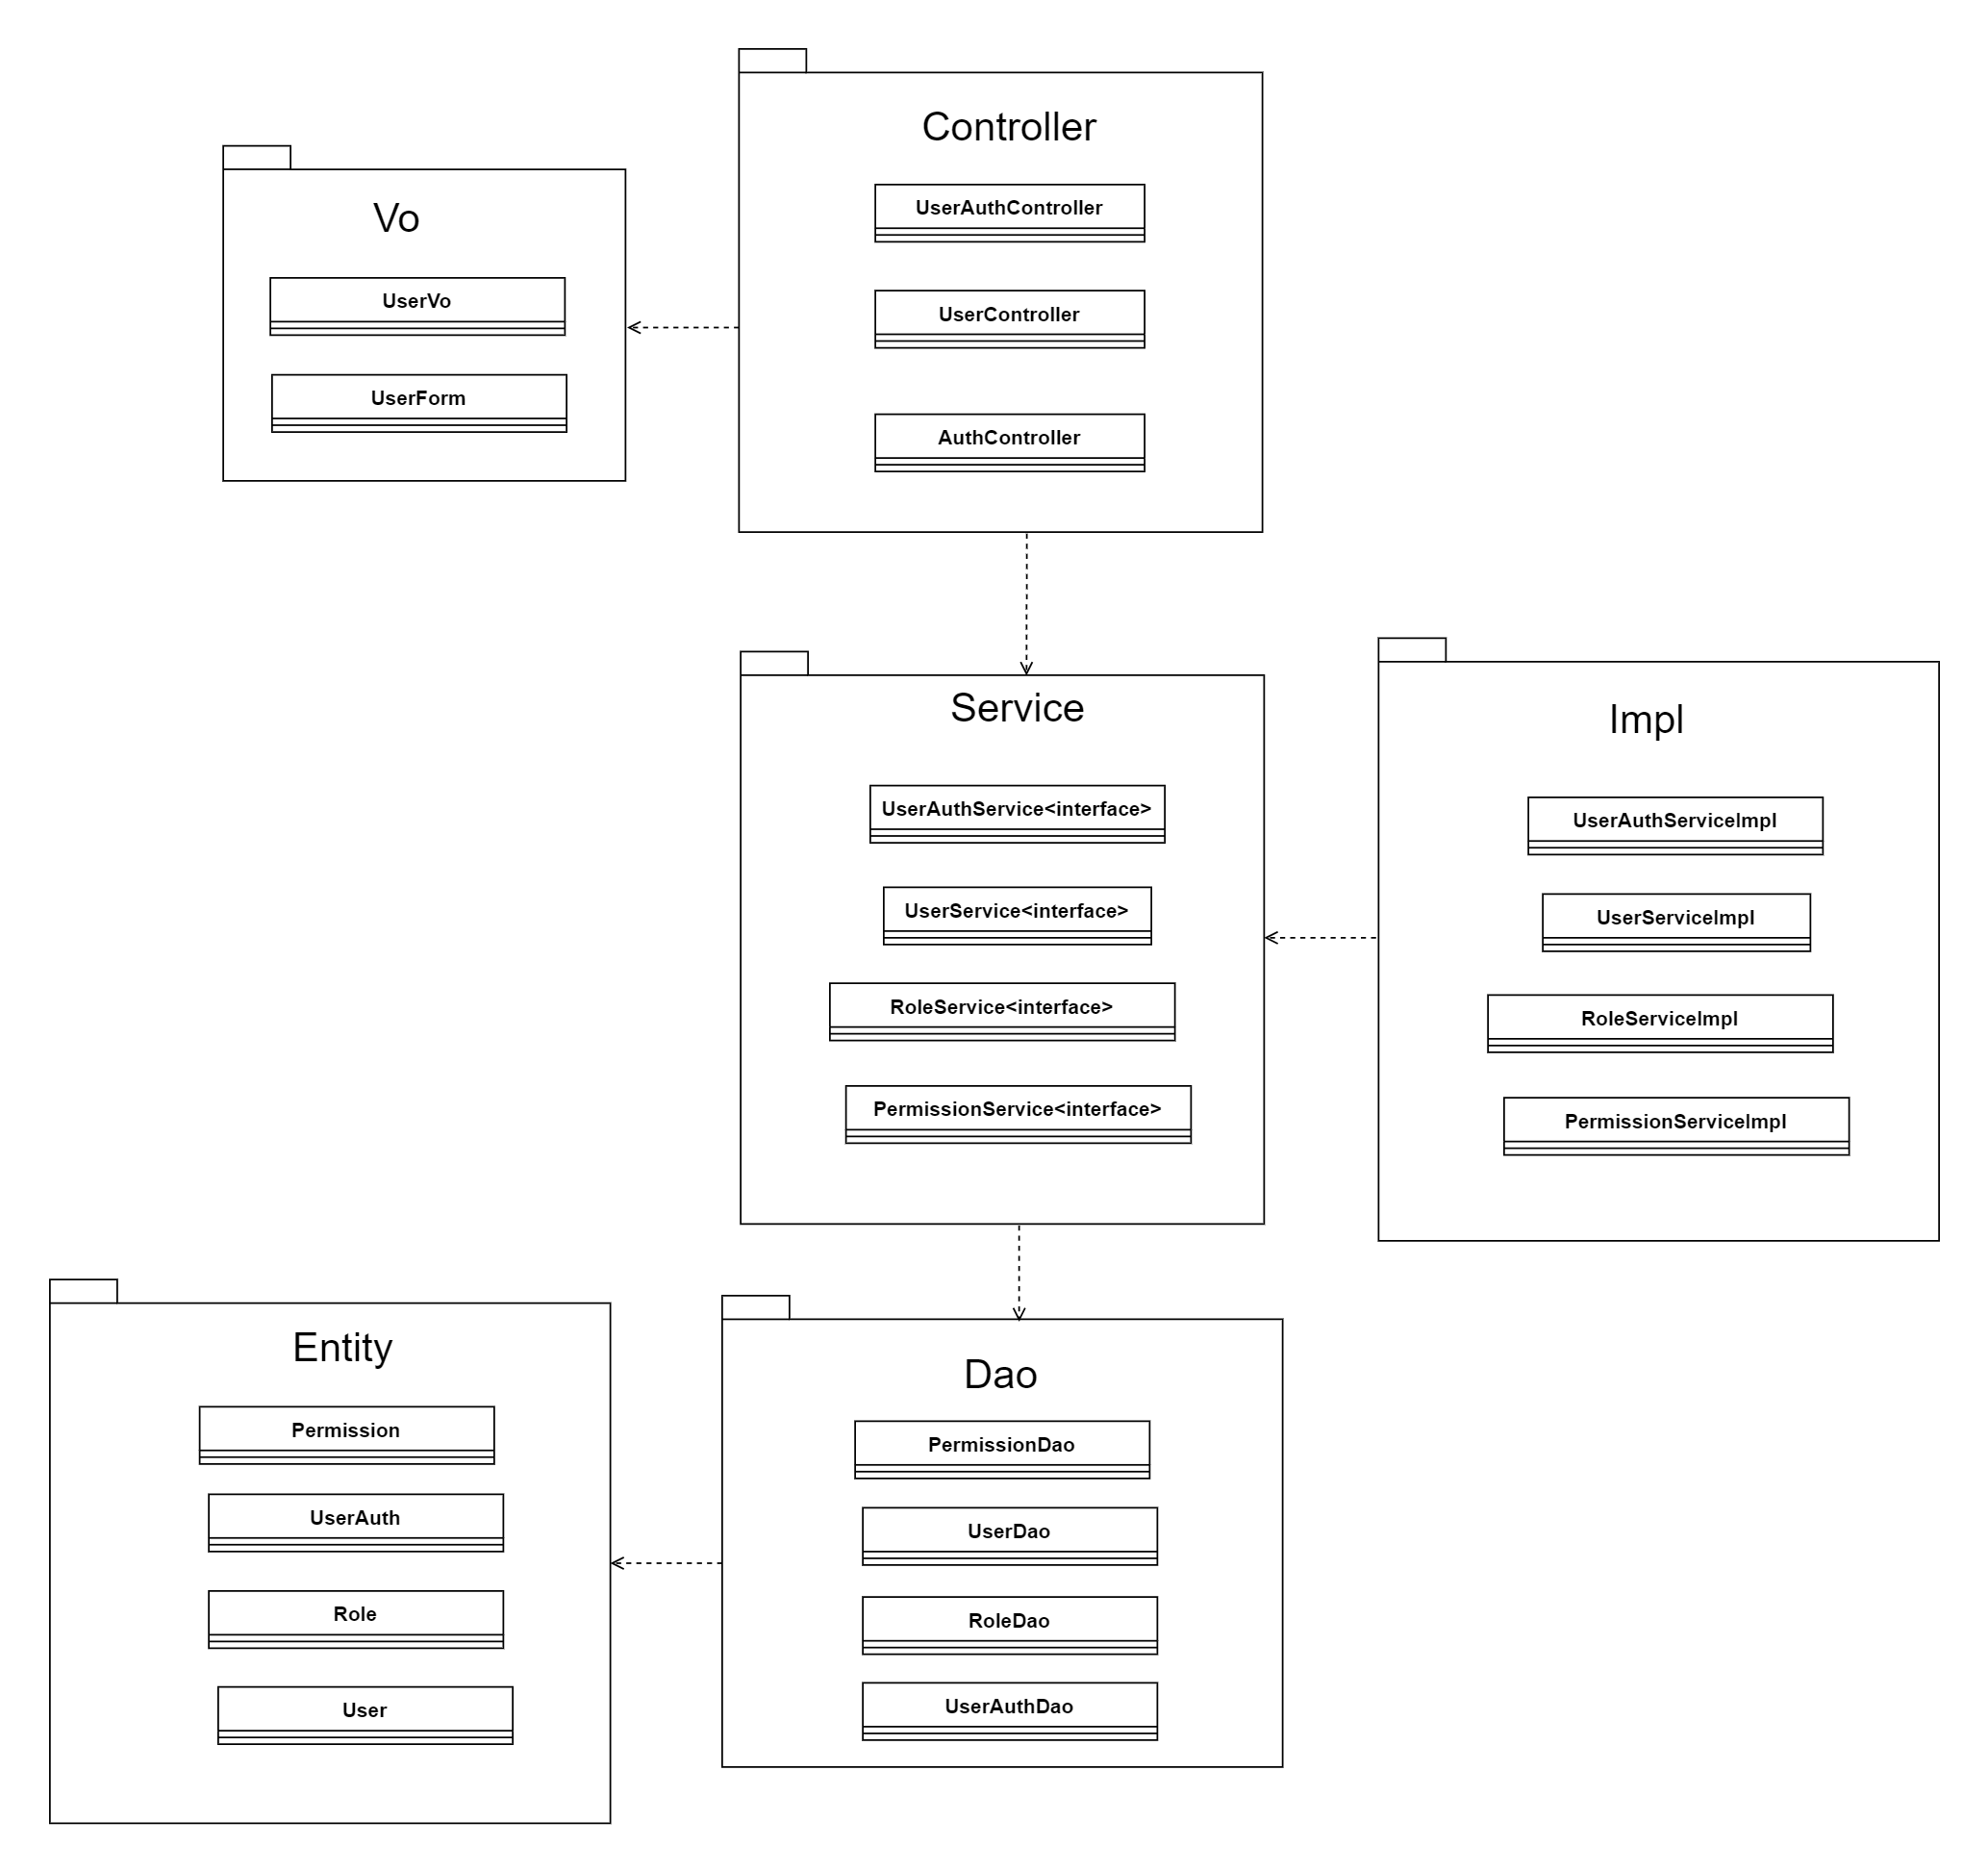
\includegraphics[width=\textwidth]{ch3/UserService.png}
    \caption{UserService模块包图}\label{fig:UserService}
    \vspace{\baselineskip} % 表示图与正文空一行
\end{figure}


\subsubsection{HouseService}
HouseService模块和上文一样,也包含6个包。总体包图如图所示。
\begin{figure}[htbp]
    \centering
    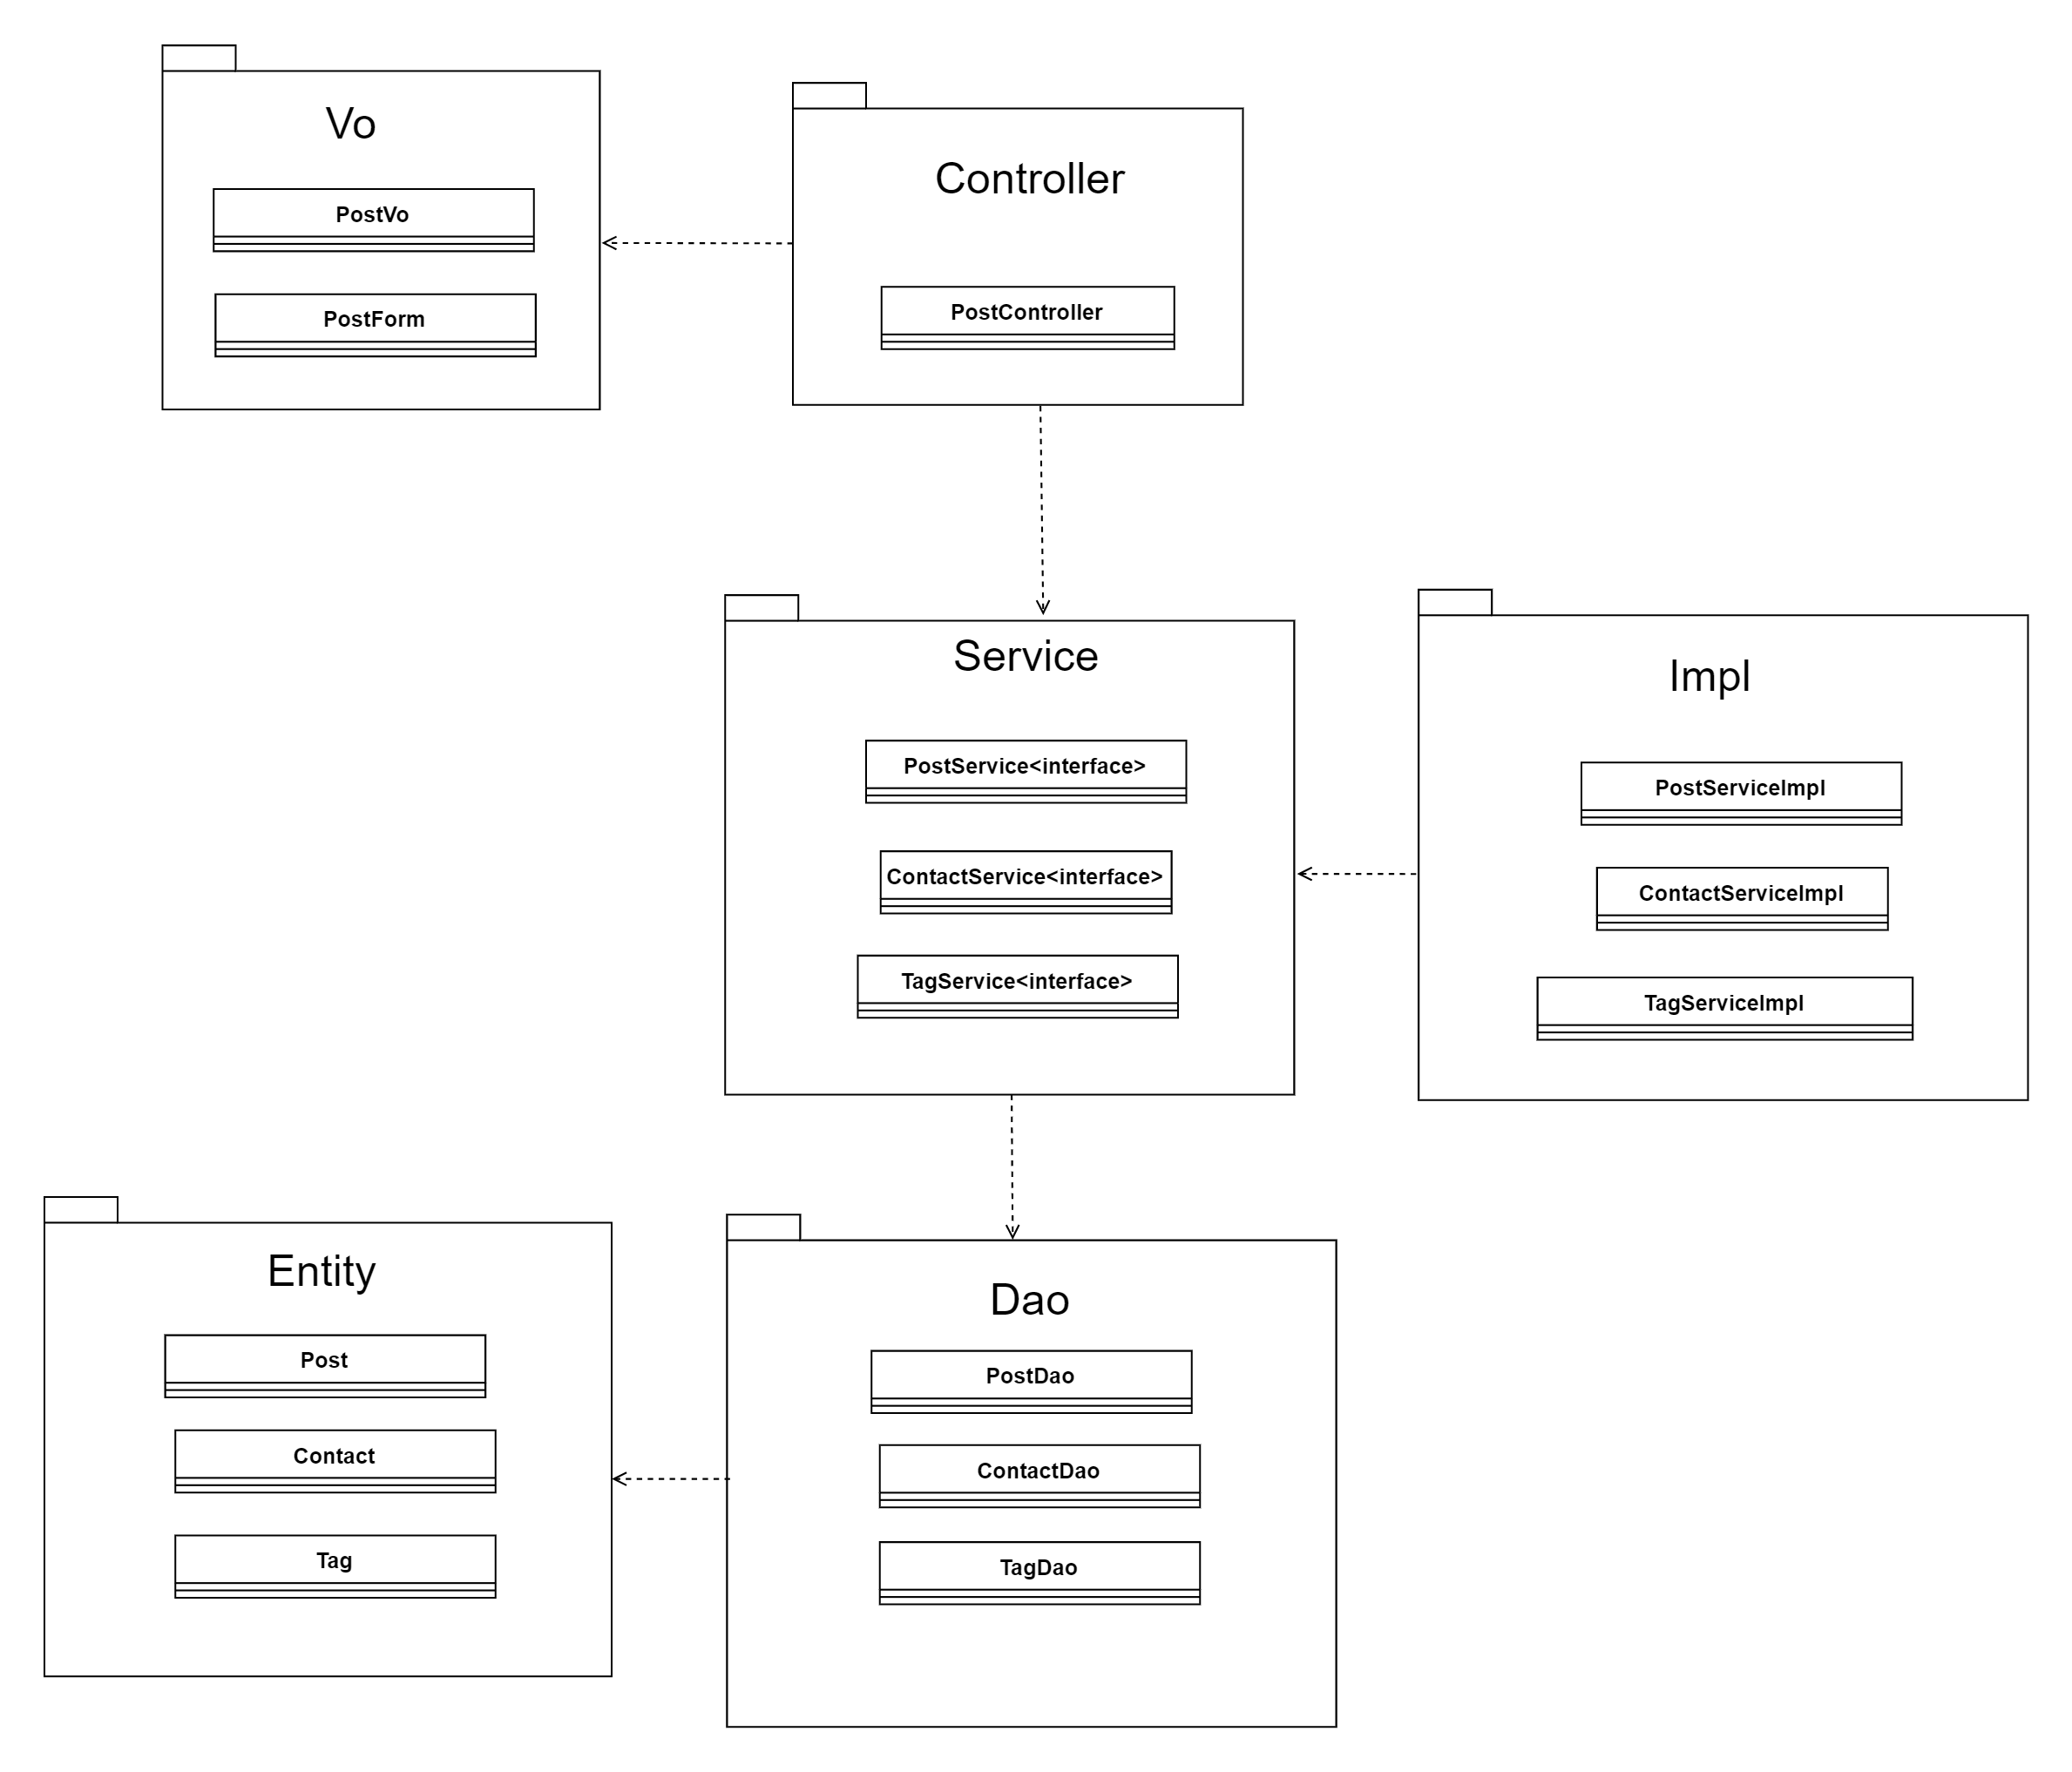
\includegraphics[width=\textwidth]{ch3/HouseService.jpg}
    \caption{HouseService模块包图}\label{fig:HouseService}
    \vspace{\baselineskip} % 表示图与正文空一行
\end{figure}

\subsubsection{NewsService}
包含6个包,总体包图如图~\ref{fig:NewsService}~所示。
\begin{figure}[htbp]
    \centering
    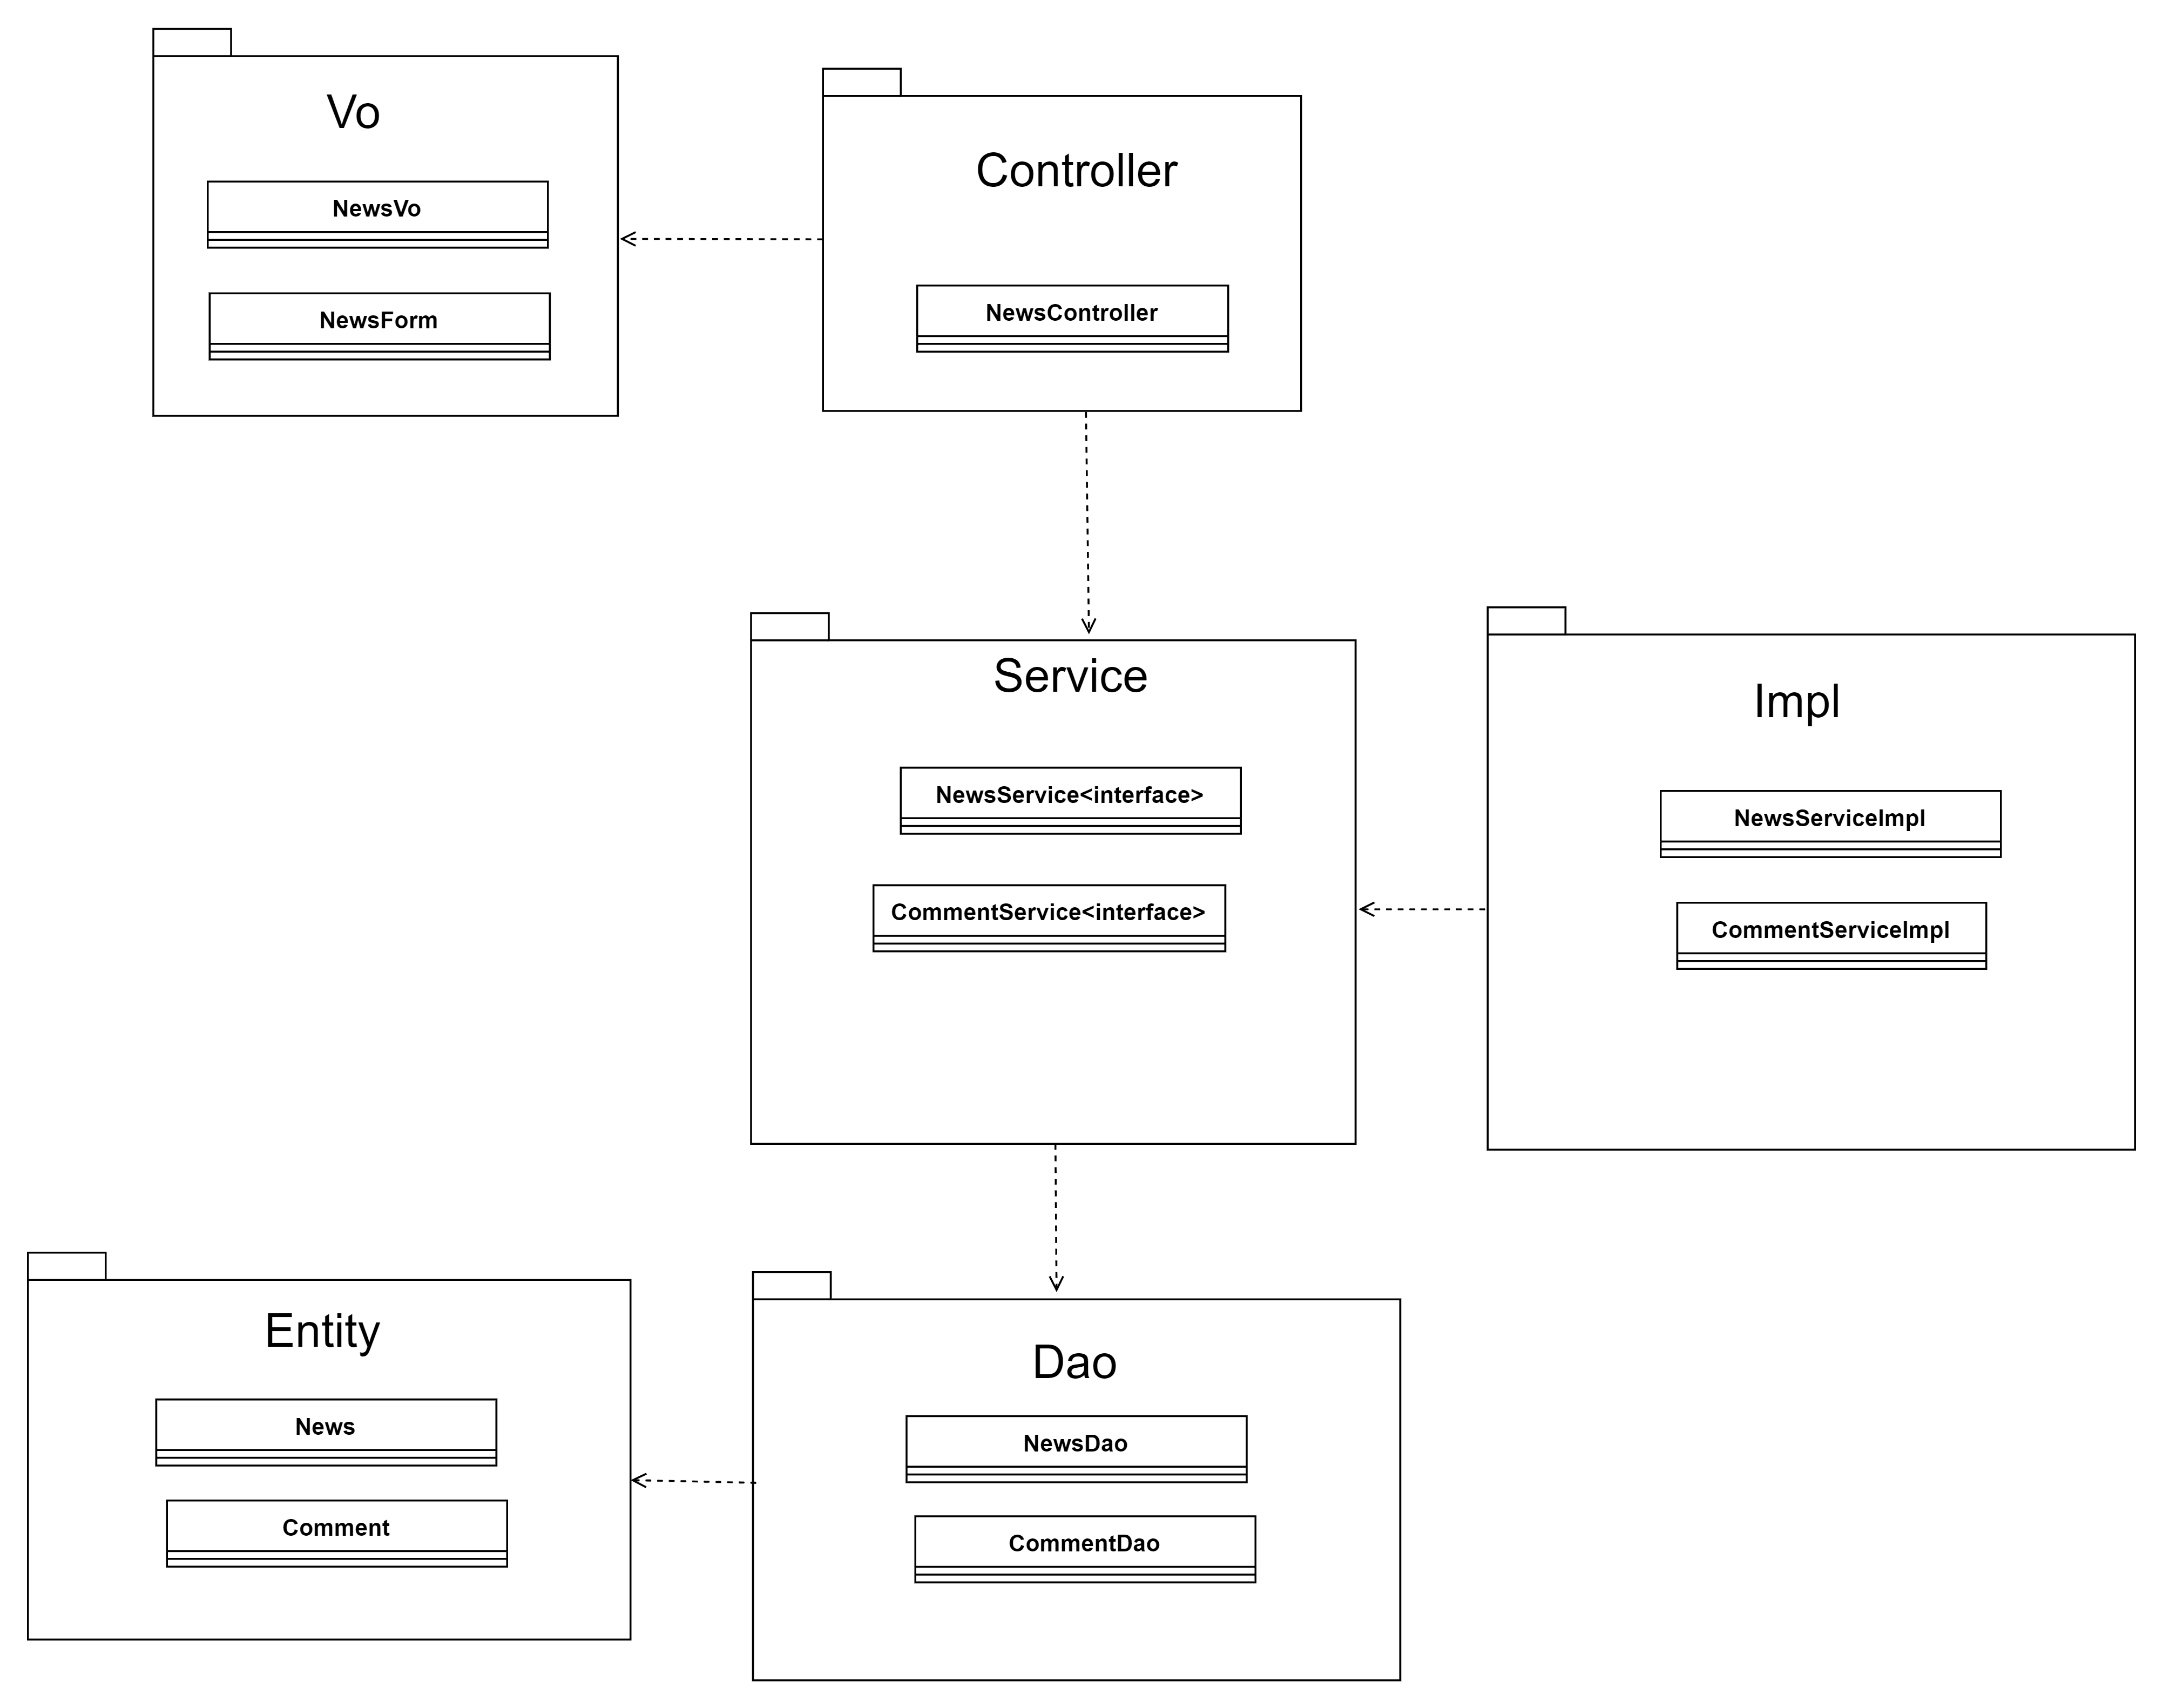
\includegraphics[width=\textwidth]{ch3/NewsService.jpg}
    \caption{NewsService模块包图}\label{fig:NewsService}
    \vspace{\baselineskip} % 表示图与正文空一行
\end{figure}

\subsubsection{ReportService}
包含6个包,总体包图如图~\ref{fig:ReportService}~所示。
\begin{figure}[htbp]
    \centering
    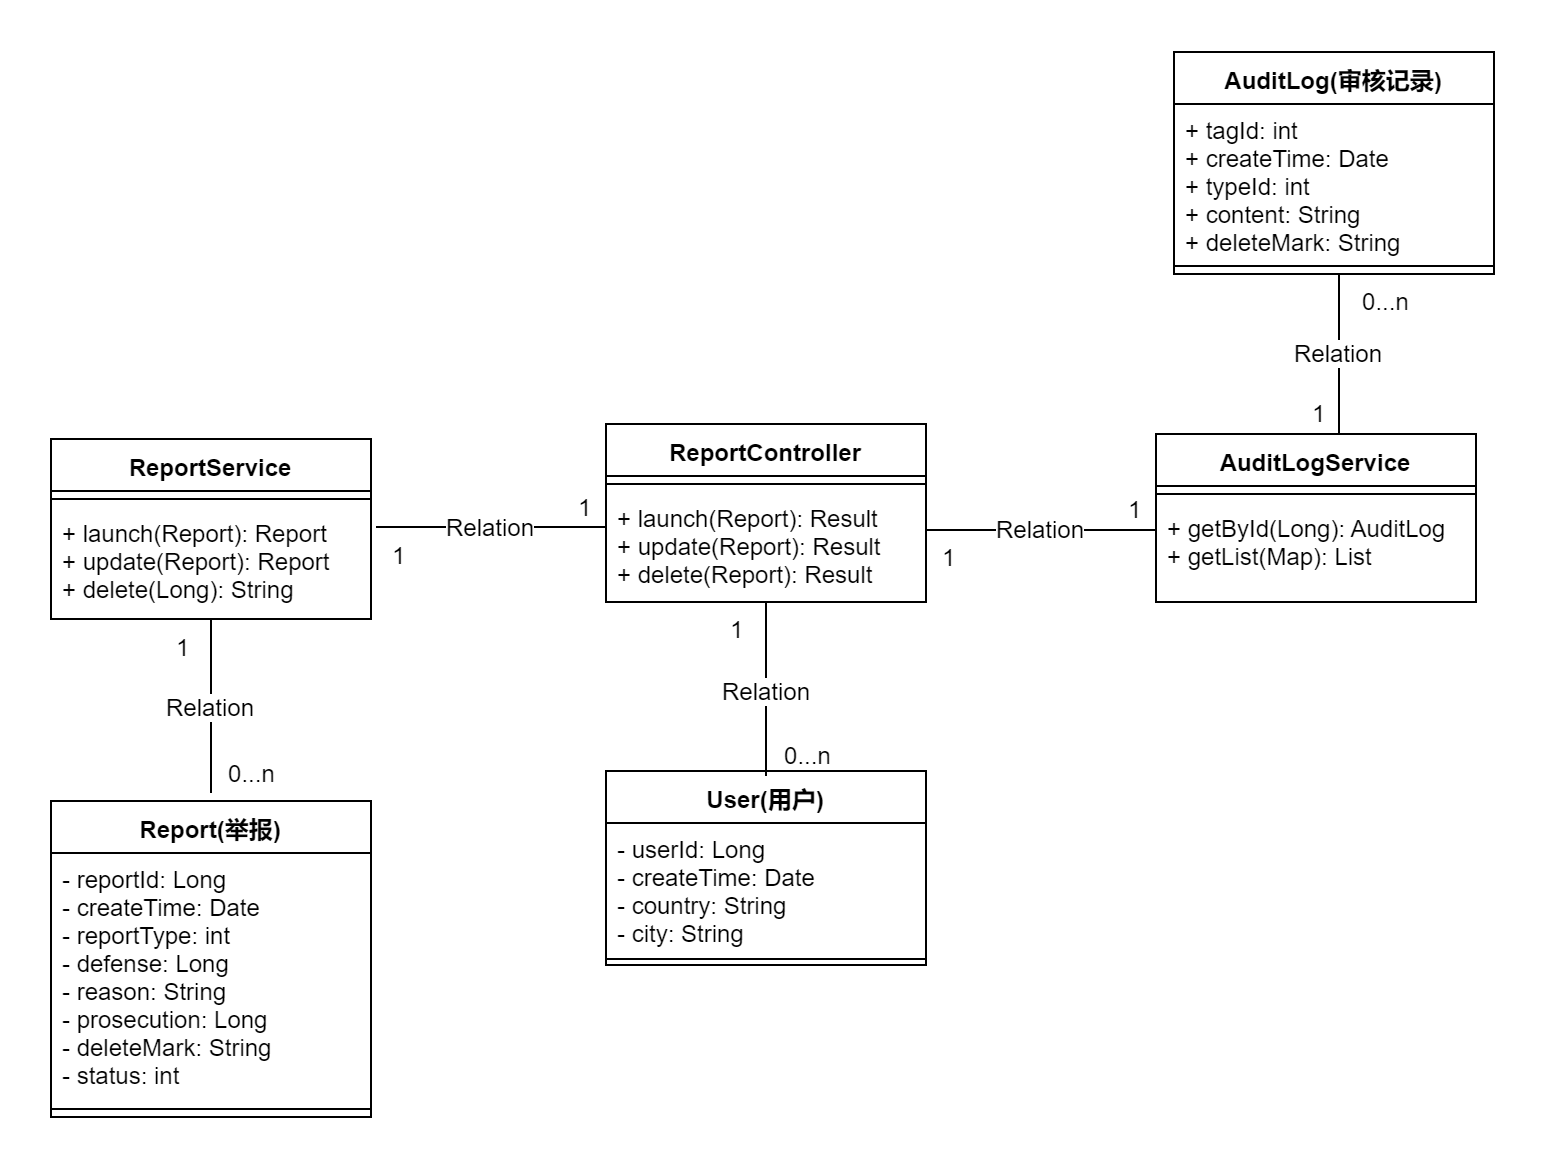
\includegraphics[width=\textwidth]{ch3/ReportService.jpg}
    \caption{ReportService模块包图}\label{fig:ReportService}
    \vspace{\baselineskip} % 表示图与正文空一行
\end{figure}

\subsubsection{AuditService}
包含6个包,总体包图如图~\ref{fig:AuditReport}~所示。
\begin{figure}[htbp]
    \centering
    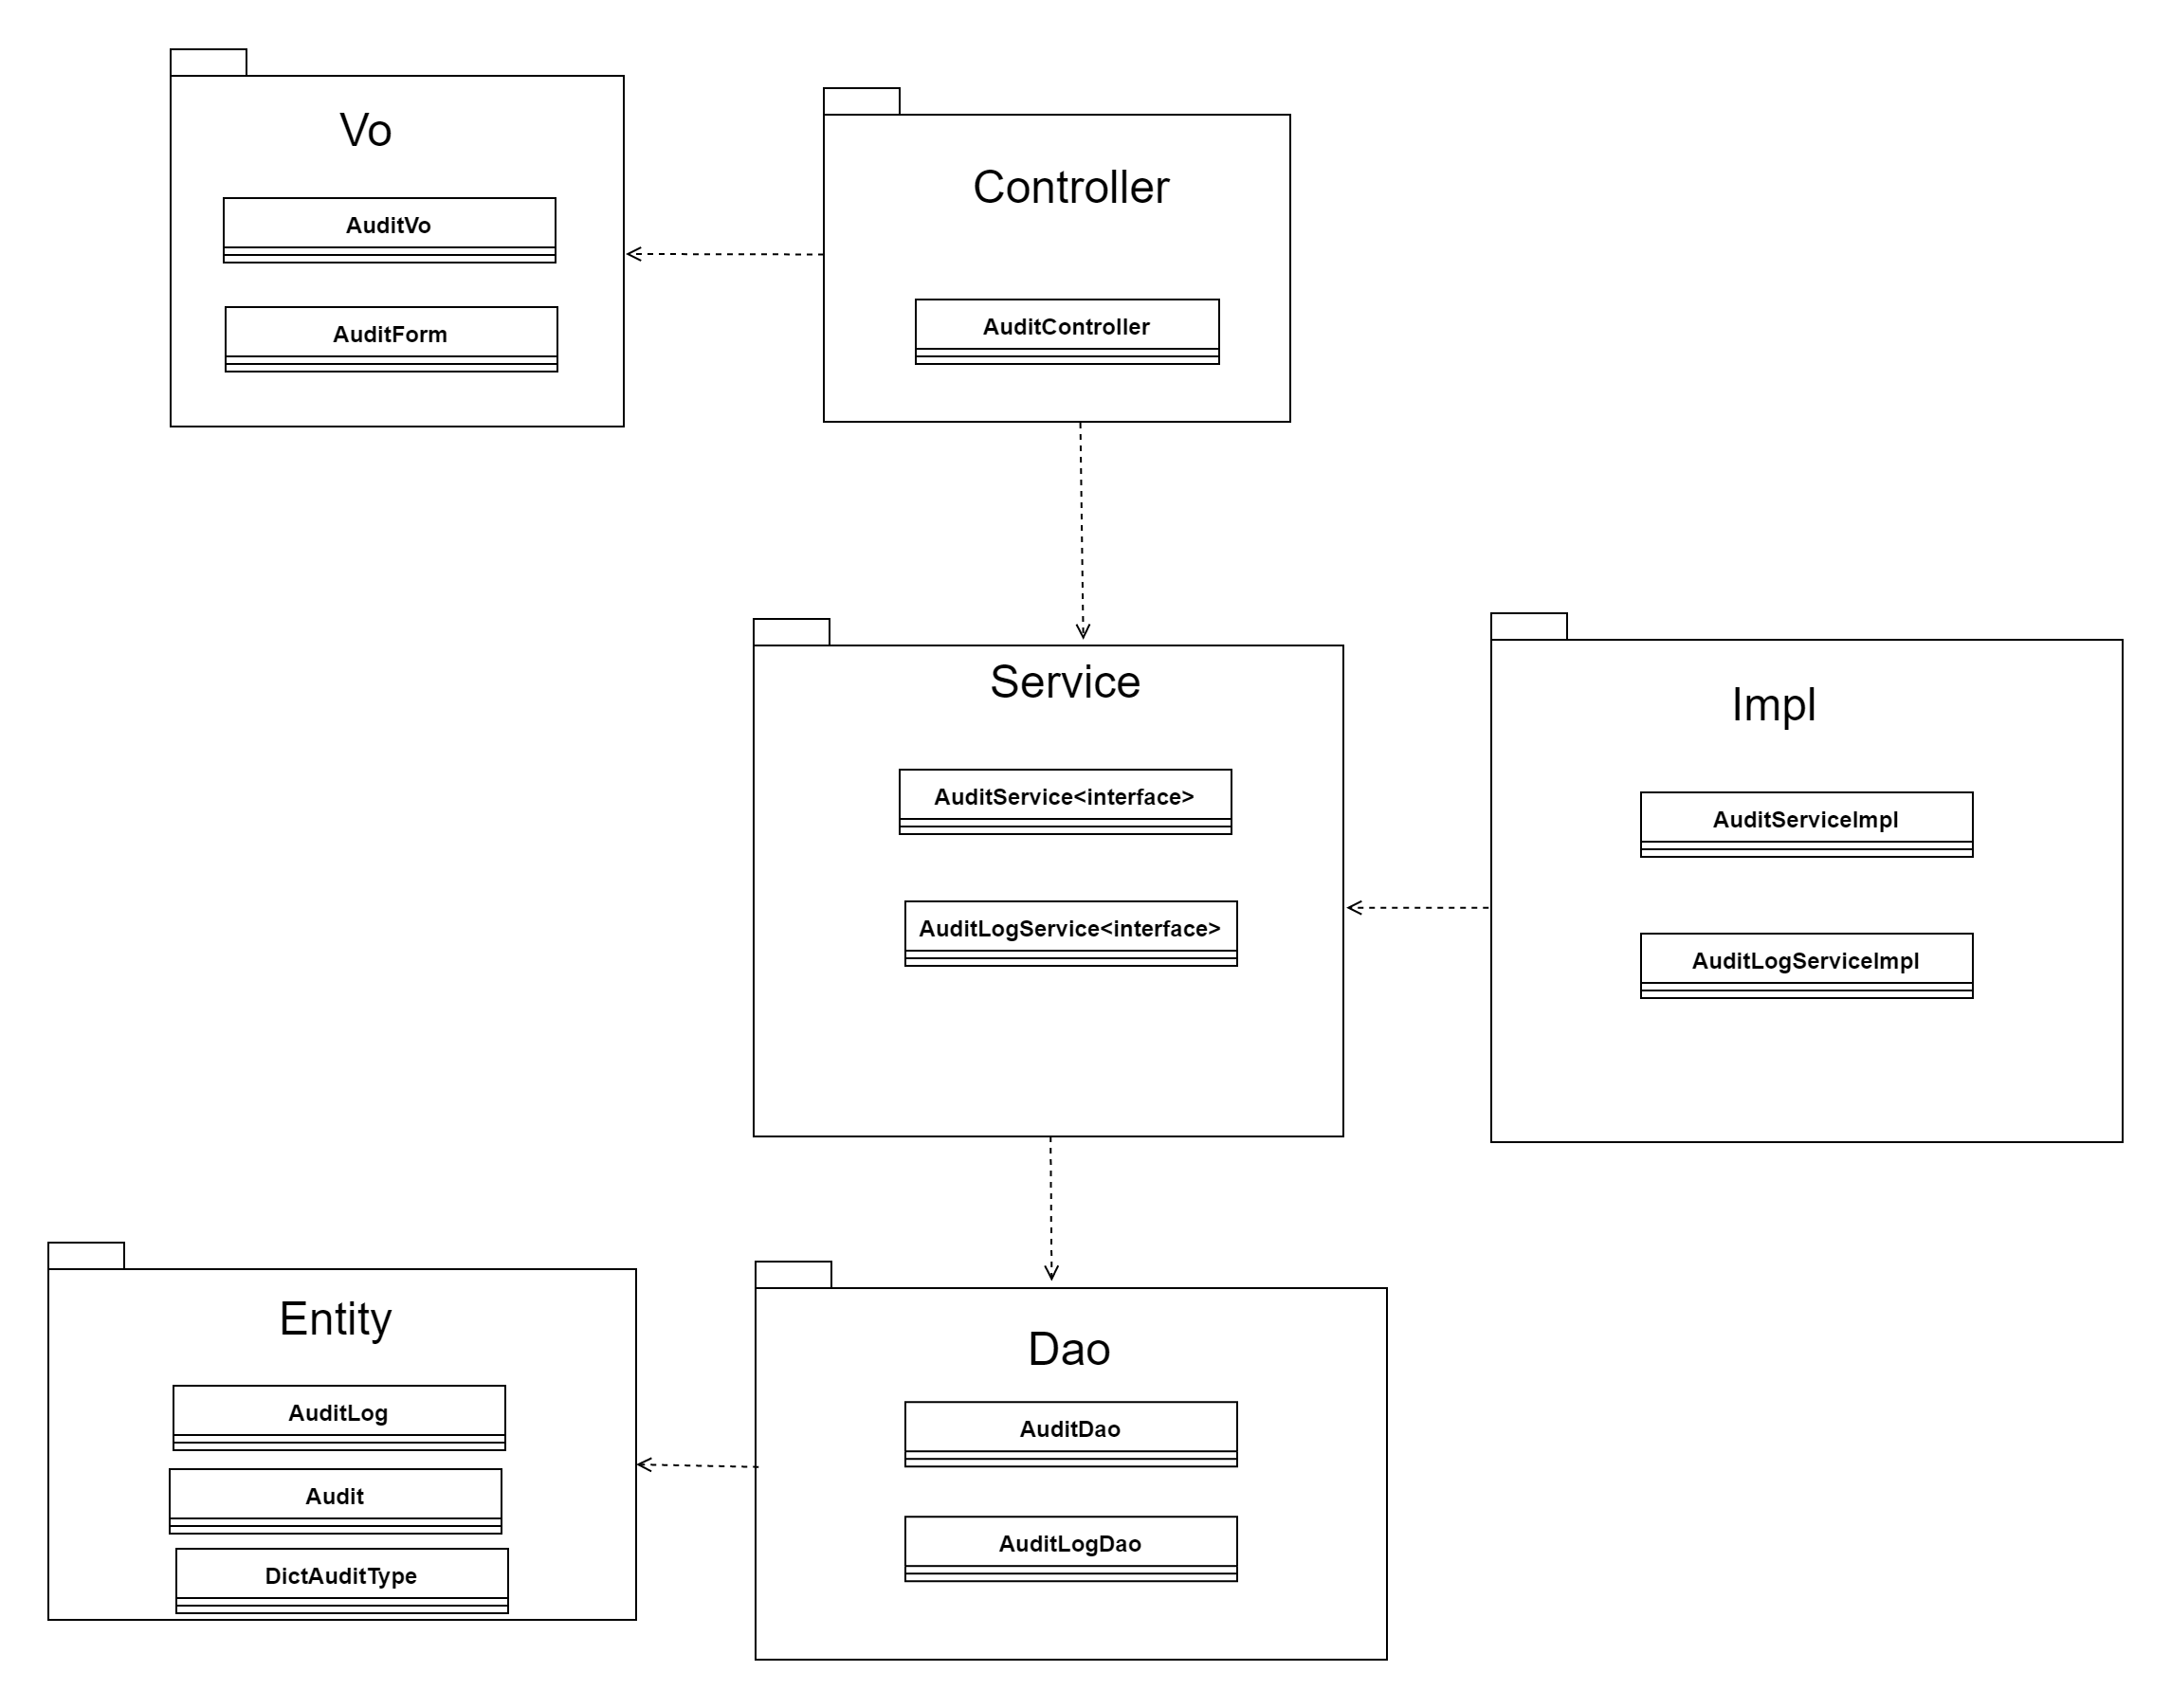
\includegraphics[width=\textwidth]{ch3/AuditService.jpg}
    \caption{AuditService模块包图}\label{fig:AuditService}
    \vspace{\baselineskip} % 表示图与正文空一行
\end{figure}

\subsubsection{SystemService}
总体包图如图~\ref{fig:SystemService}~所示。
\begin{figure}[htbp]
    \centering
    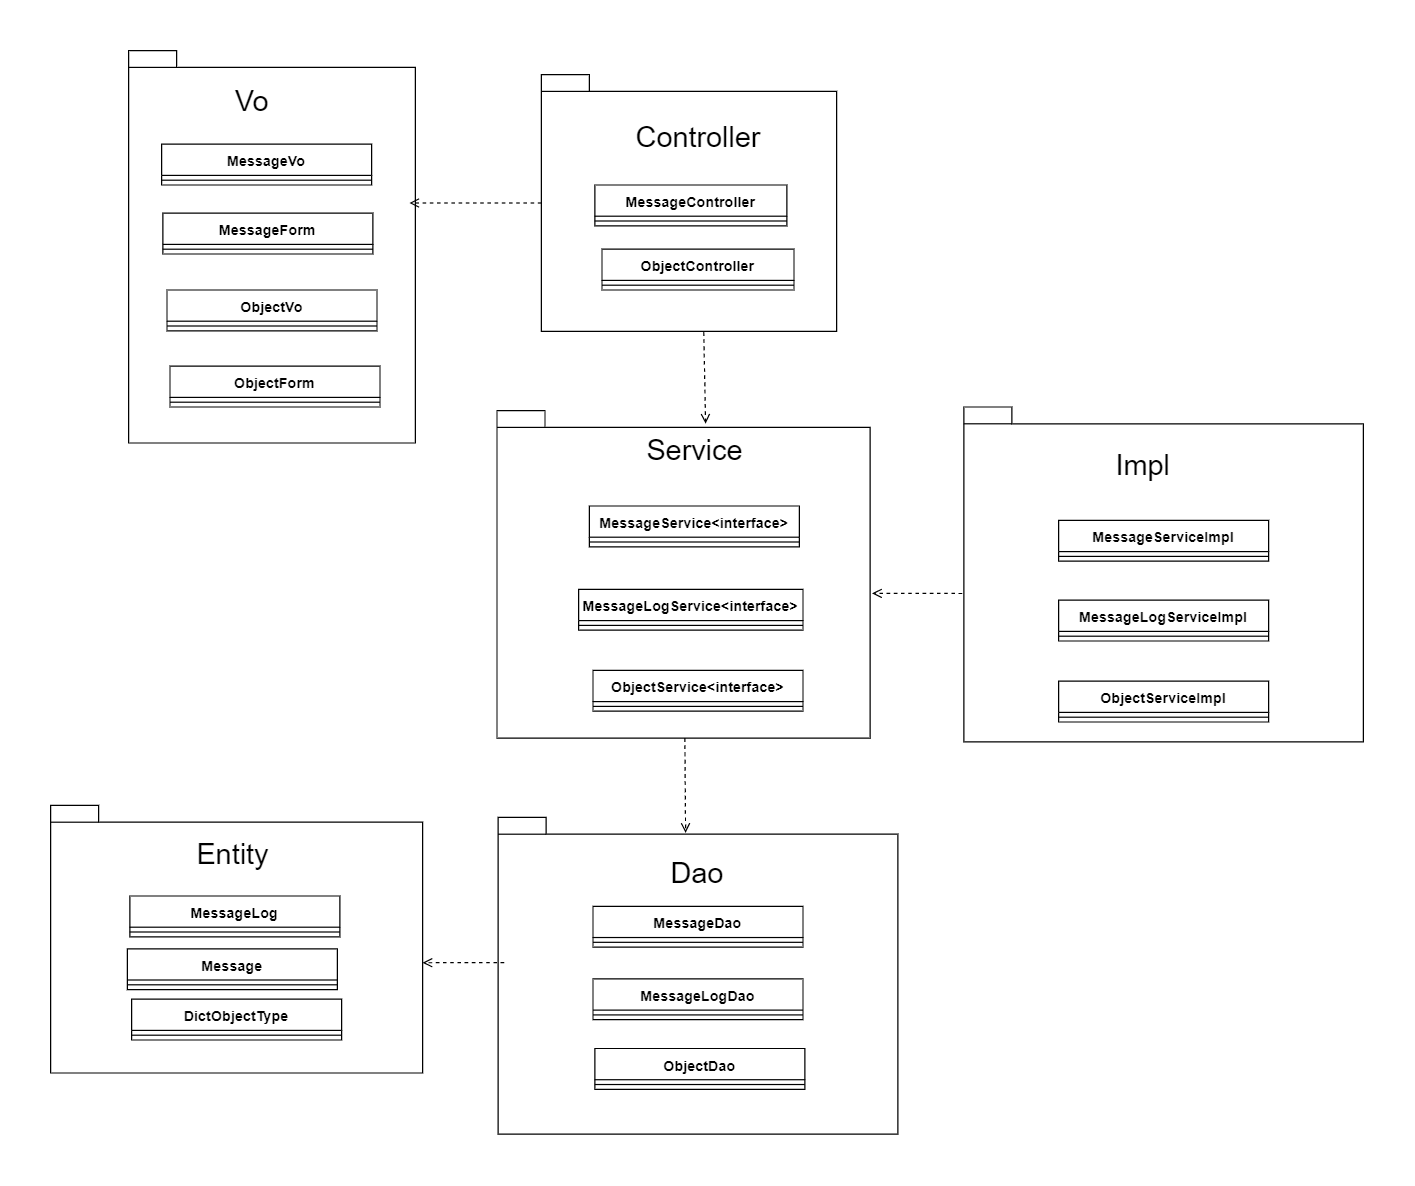
\includegraphics[width=\textwidth]{ch3/SystemService.jpg}
    \caption{SystemService模块包图}\label{fig:SystemService}
    \vspace{\baselineskip} % 表示图与正文空一行
\end{figure}


\subsection{GateWay网关模块}
GateWay网关模块负责路由转发,同时还负责初步的用户权限检查。所谓的网关权限检查,即对于用户的登陆凭证token进行初步检验。由于路由转发功能在配置文件中
已经实现,需要自定义的权限检查只需要一个包即可。下面为GateWay网关模块的包图~\ref{fig:GateWay}~。
\begin{figure}[htbp]
    \centering
    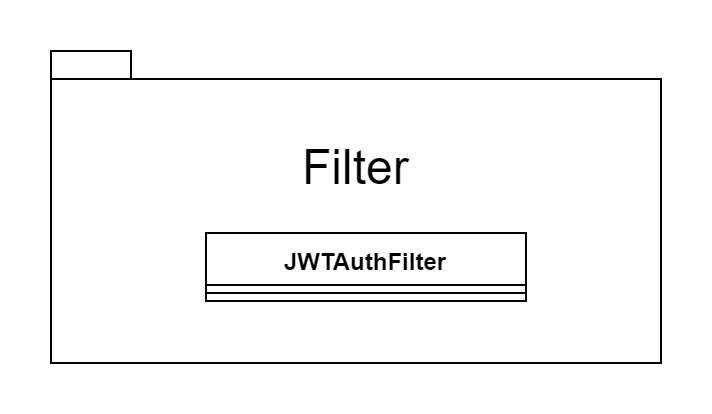
\includegraphics[width=0.7\textwidth]{ch3/GateWay.jpg}
    \caption{GateWay模块包图}\label{fig:GateWay}
    \vspace{\baselineskip} % 表示图与正文空一行
\end{figure}

\subsection{系统部署图}
本系统的部署主要涉及到服务端、客户端和数据库。客户端主要为Web浏览器,服务端需要部署多个微服务,同时启动Redis服务,数据库使用MySQL数据库。
系统部署图如图~\ref{fig:goujian}~所示。
\begin{figure}[htbp]
    \centering
    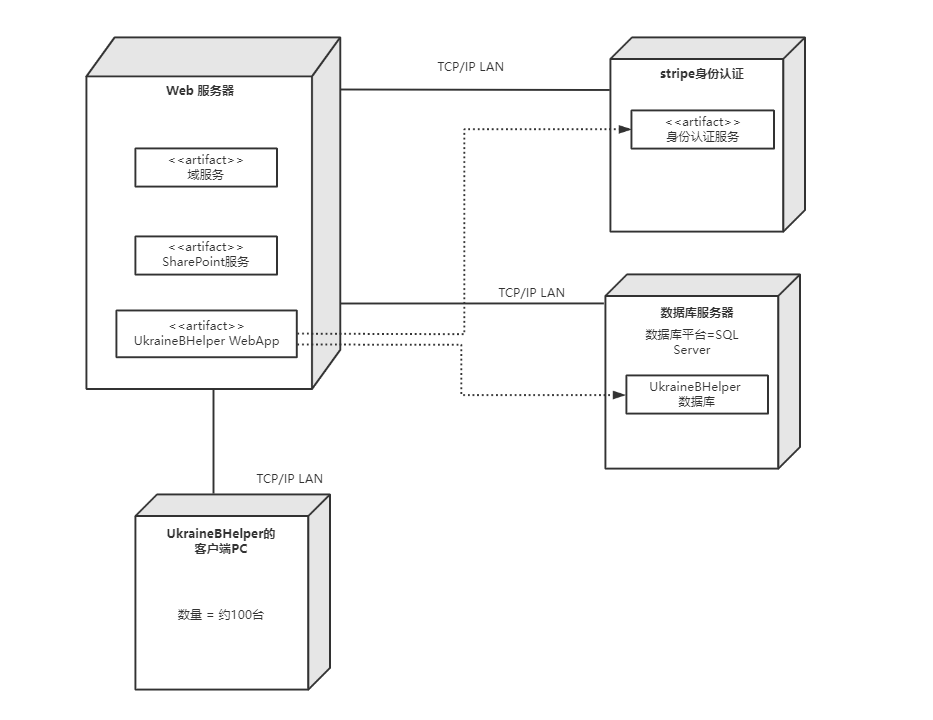
\includegraphics[width=\textwidth]{ch3/goujian.png}
    \caption{系统部署图}\label{fig:goujian}
    \vspace{\baselineskip} % 表示图与正文空一行
\end{figure}
\chapter{接口说明}
本章将对系统中的应用的接口,包括interface,abstract class进行详细说明,主要在于说明他们的public方法,以及方法中参数的意义和返回值的意义。

\section{Security模块}
为了便于扩展不同的认证授权方案,Security模块定义了许多认证授权操作的接口,以及相关过滤器的抽象类,包括登录过滤器、授权过滤器、用户加载接口等。
\subsection{UsernamePasswordAuthenticationFilter}
此抽象类为登录时调用的过滤器类。类中共定义了3个主要方法,作用分别为用户认证、认证成功和认证失败。
\begin{itemize}
    \item attemptAuthentication方法,返回类型为Authentication(用户认证类),参数有2个,类型分别为HttpServletRequest、HttpServletResponse。方法用途为将request中的用户信息进行校验。
    \item successfulAuthentication方法,返回类型为void,参数有4个,类型分别为HttpServletRequest、HttpServletResponse、Authentication、FilterChain(过滤链)。方法用途为用户认证成功后进行相关操作,包括加载权限等,然后将用户认证信息通过过滤链传递给下个过滤器。
    \item unsuccessfulAuthentication方法,返回类型为void,参数有3个,类型分别为HttpServletRequest、HttpServletResponse、Authentication。方法用途为用户认证失败后进行相关操作,包括返回失败信息等。
\end{itemize}

\subsection{BasicAuthenticationFilter}
此抽象类为授权时调用的过滤器类,类中需要说明的方法主要有1个,作用是获取用户权限,然后交给鉴权过滤器去鉴权。
\begin{itemize}
    \item doFilterInternal方法,返回类型为void,参数有3个,类型分别为HttpServletRequest、HttpServletResponse、FilterChain。方法用途为将request中的用户进行权限加载,然后把权限信息交给鉴权过滤器去鉴权。
\end{itemize}

\subsection{AccessDeniedHandler}
此接口定义了用户权限不够时所调用方法。主要的方法有1个,作用是设置用户权限不足的信息,然后将其返回给用户。
\begin{itemize}
    \item handle方法,返回类型为void,参数有3个,类型分别为HttpServletRequest、HttpServletResponse、AccessDeniedException(权限异常类)。方法用途为在HttpServletResponse中设置用户权限不足的信息并返回给用户。
\end{itemize}

\subsection{AuthenticationEntryPoint}
此接口定义了用户认证失败时所调用方法。主要的方法有1个,作用是设置用户认证失败的信息,然后将其返回给用户。
\begin{itemize}
    \item commence方法,返回类型为void,参数有3个,类型分别为HttpServletRequest、HttpServletResponse、AuthenticationException(认证异常类)。方法用途为在HttpServletResponse中设置用户认证失败的信息并返回给用户。
\end{itemize}

\subsection{PasswordEncoder}
此接口定义了用户密码加密和匹配的策略,主要有2个方法,作用分别是用户密码的加密算法和用户密码的匹配算法。
\begin{itemize}
    \item encode方法,返回类型为String,参数有1个,类型为CharSequence(用户传来的原始密码),作用在于对用户输入的密码进行加密计算,至于加密密码可以自定义,比如md5加密等。
    \item matches方法,返回类型为Boolean,参数有2个,类型都是CharSequence,分别表示用户输入的密码和数据库查询的密码,然后通过自定义的匹配算法进行匹配。
\end{itemize}

\subsection{UserDetailsService}
此接口定义了用户详细信息的加载方法,主要是1个方法,作用为从数据库加载用户的基本信息、角色信息和权限信息,并进行用户登录初始化工作。
\begin{itemize}
    \item loadUserByUsername方法,返回类型为UserDetail,参数有1个,类型分别为String,表示登录用户的用户名。方法用途为根据传入的用户名从数据库加载用户基本信息、角色信息和权限信息,并进行初始化工作,比如权限信息存入Redis缓存等。
\end{itemize}

\section{GateWay模块}
因为GateWay网关是需要处理客户端发来的一切请求,我们需要自定义一些过滤器。为了可扩展性,需要一个全局的过滤器类,实现过滤器的扩展。
\subsection{GlobalFilter}
此接口定义了过滤器实际过滤采用的方法,主要方法有1个,作用是接收并预处理客户端发来的一切请求。
\begin{itemize}
    \item filter方法,返回类型为Mono<void>,参数有2个,类型分别为ServerWebExchange(客户端请求)、GatewayFilterChain(网关过滤器链)。方法用途为将客户端请求进行预处理,如果符合要求则放行,否则返回错误信息。
\end{itemize}

\section{Service模块}
Service是业务模块,用的是MVC的框架,其中将每个具体的业务方法都进行了interface+impl的组合,即每个业务方法都被抽象成了一个接口,这样的话
我们需要进行扩展就只需要新建impl即可,增加了系统的可扩展性。


\chapter{业务对象及相互关系}
\section{概述}
本系统的主要业务模块分为房源管理,新闻管理,用户权限管理,系统管理,技术模块分为前端技术和后端技术,技术栈为:
\begin{itemize}
    \item 后端技术: SpringCloud + SpringSecurity + Nacos + OpenFeign + Spring Gateway + Mybatis-plus + MySQL
    \item 前端技术: 
\end{itemize}
\section{业务概念一览}
本系统的模块可以详细分为用户、角色、权限、房源、新闻、信息、举报、审核、日志、通讯这十个模块。下图为这几个模块的关系类图。
\begin{figure}[htbp]
    \centering
    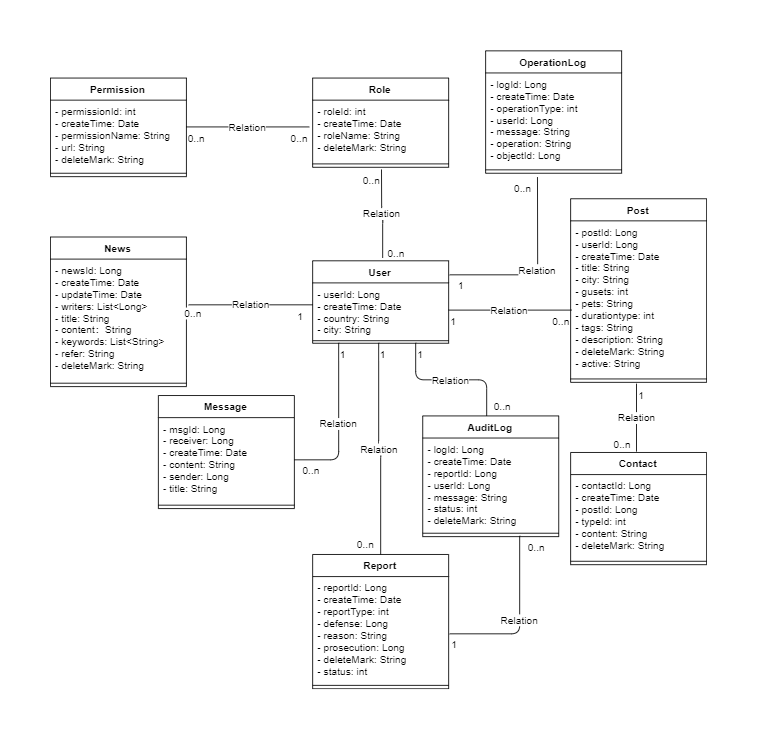
\includegraphics[width=1\textwidth]{ch5/AkraineHelper.png}
    \caption{总类图}\label{fig:AkraineHelper}
    \vspace{\baselineskip} % 表示图与正文空一行
\end{figure}
\section{登录}
登录是个较为复杂的模块,因为他需要认证用户信息,生成用户登录凭证,还需要将用户的权限信息存入缓存中以便后续的鉴权工作。

登录模块使用了SpringSecurity架构,其中我们自定义了登陆用户信息,还有一些相关过滤器,同时我们使用了SpEL语言在AuthCheckeService中重定义了系统的鉴权规则,使得系统动态
匹配用户权限信息。同时用户密码的加密,以及登陆凭证的生成都是根据项目实际情况自行定义的,其类图关系如下。
\begin{figure}[htbp]
    \centering
    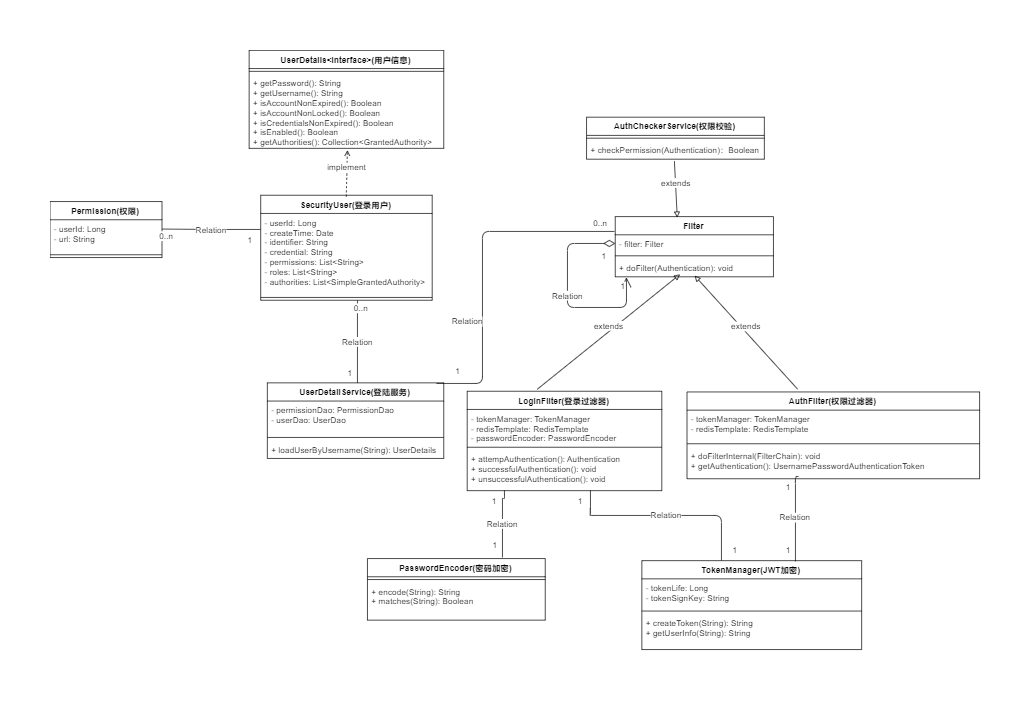
\includegraphics[width=1\textwidth]{ch5/Authentication.png}
    \caption{登录}\label{fig:Authentication}
    \vspace{\baselineskip} % 表示图与正文空一行
\end{figure}
\section{发布房源}
房源发布主要为屋主的操作,该模块要求屋主填写填写房源基本信息,包括房源地址,容纳人数,是否允许宠物等,还需要屋主留下联系方式,难民可以根据联系方式
自行去联系屋主。涉及到的实体类有用户类(User),帖子类(Post),联系方式(Contact),标签(Tag)。具体的方法都在PostController中进行调用。
\begin{figure}[htbp]
    \centering
    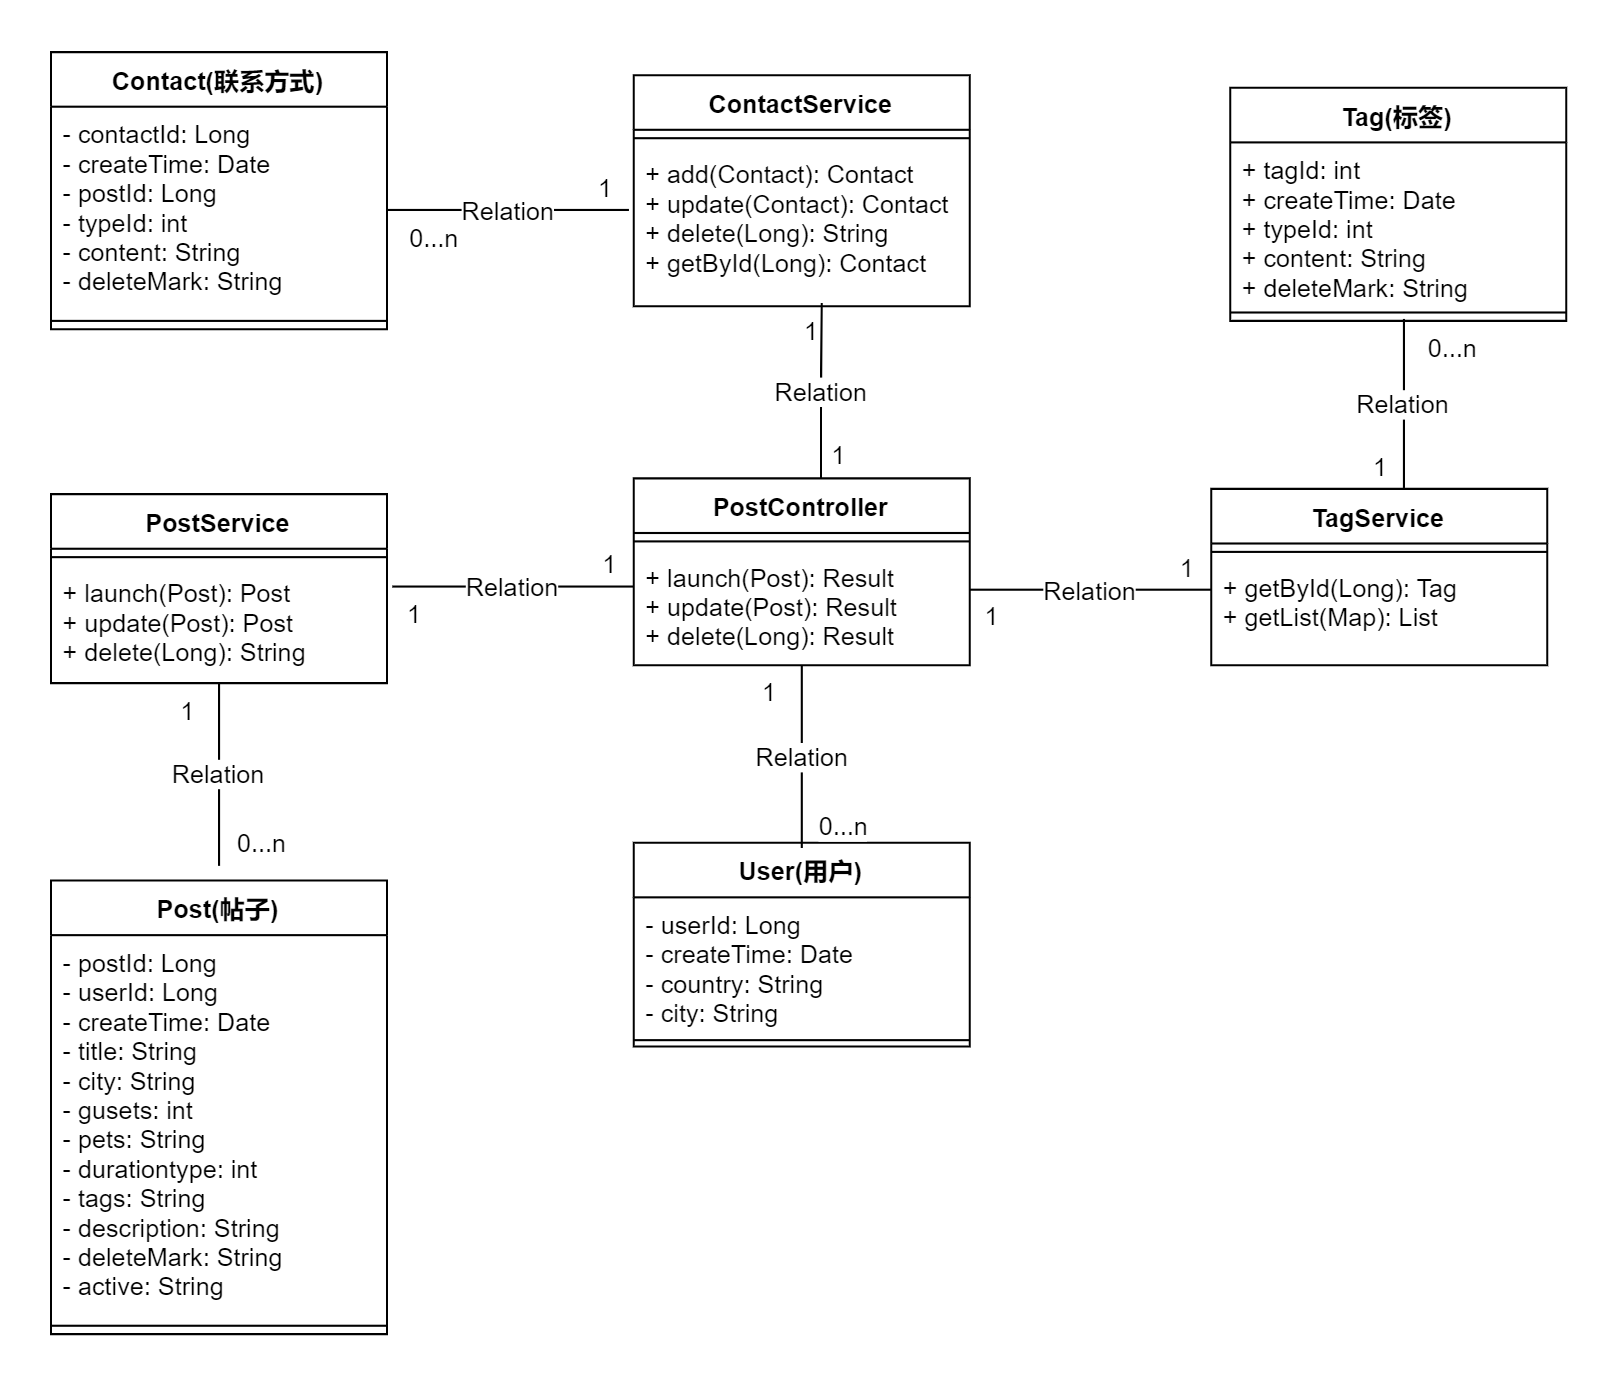
\includegraphics[width=1\textwidth]{ch5/LaunchPost.png}
    \caption{发布房源}\label{fig:LaunchPost}
    \vspace{\baselineskip} % 表示图与正文空一行
\end{figure}
\section{修改房源}
屋主可以查看自己发布的房源,然后进行修改,比如添加删除标签,修改联系方式等等,具体的方法还是在PostController中调用。
\begin{figure}[htbp]
    \centering
    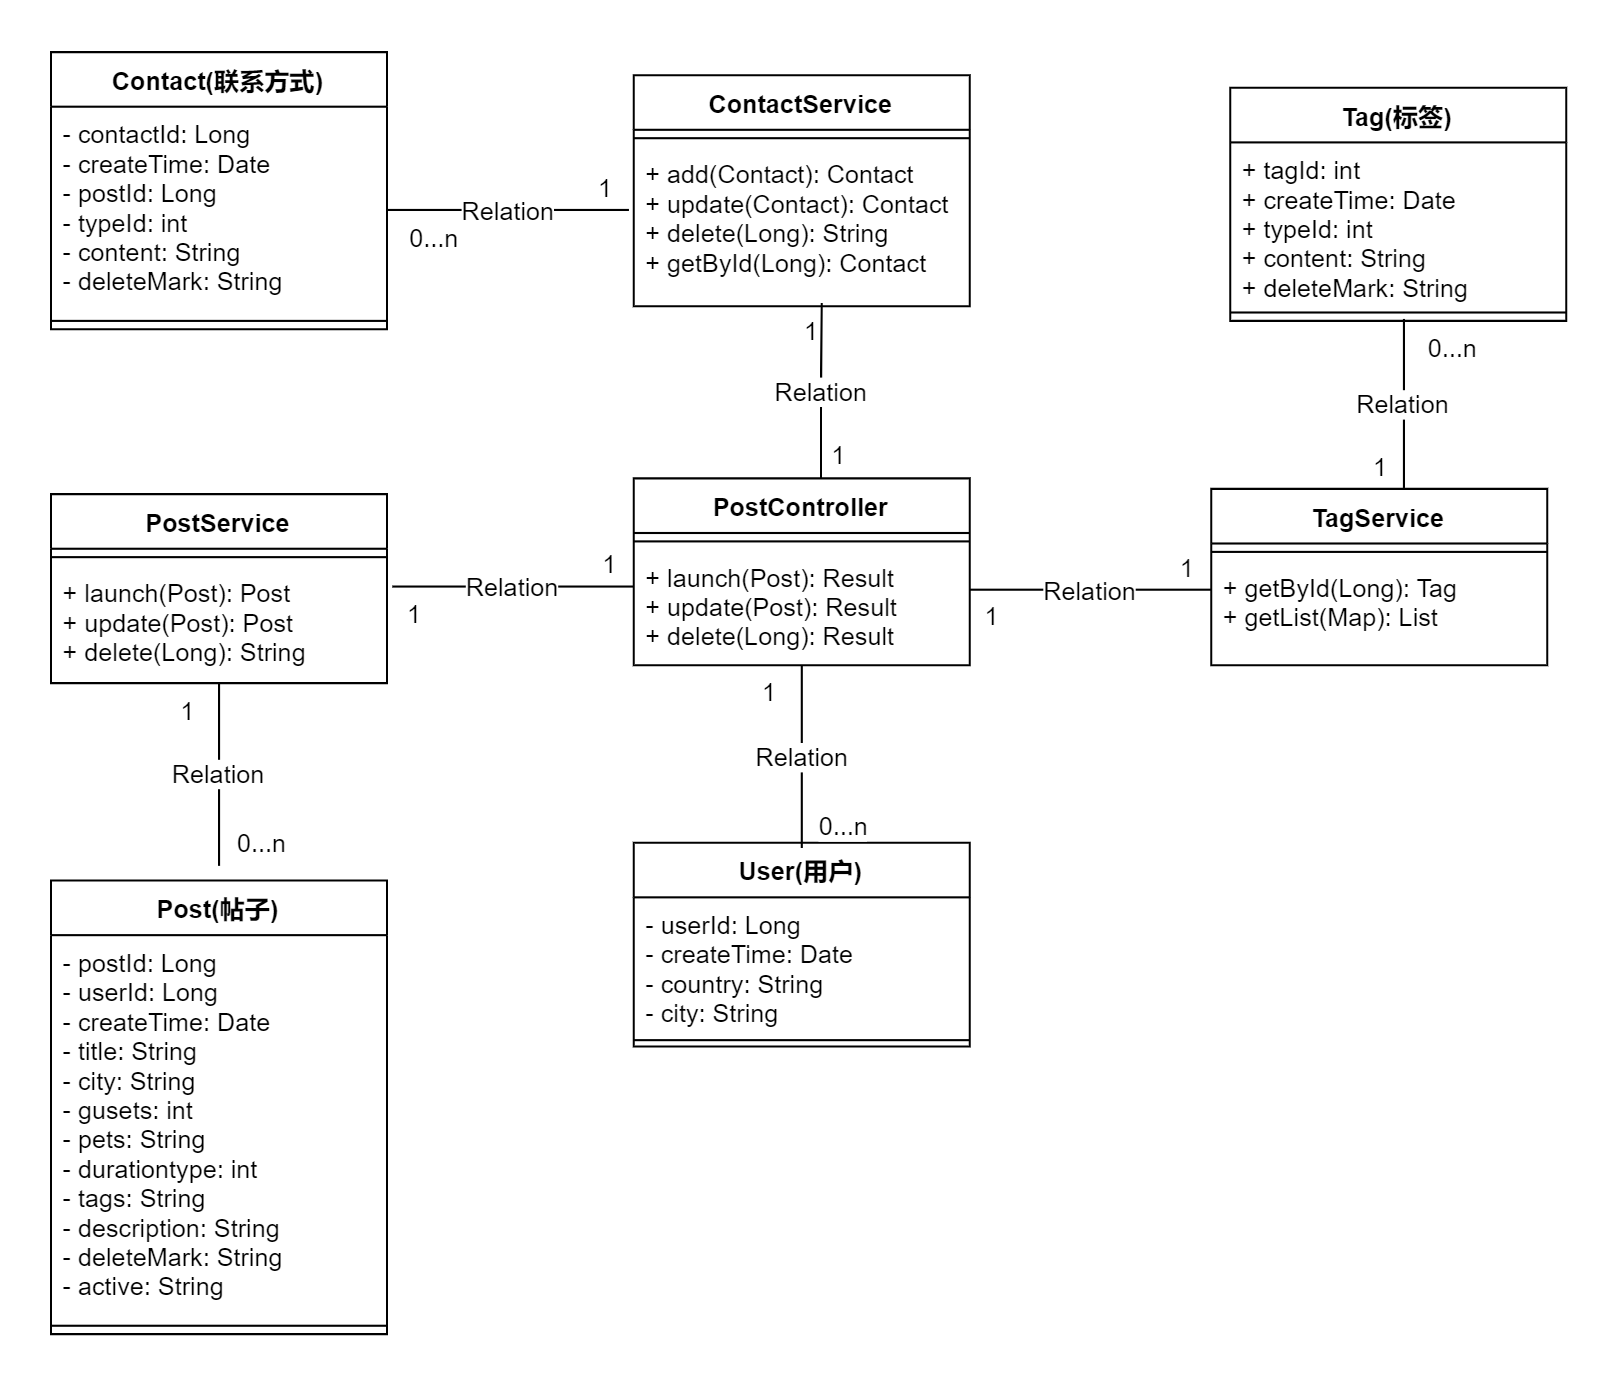
\includegraphics[width=1\textwidth]{ch5/LaunchPost.png}
    \caption{修改房源}\label{fig:UpdatePost}
    \vspace{\baselineskip} % 表示图与正文空一行
\end{figure}
\section{删除房源}
屋主可以查看自己发布的房源,然后进行删除操作,就可以将发布过的房源不再显示。
\begin{figure}[htbp]
    \centering
    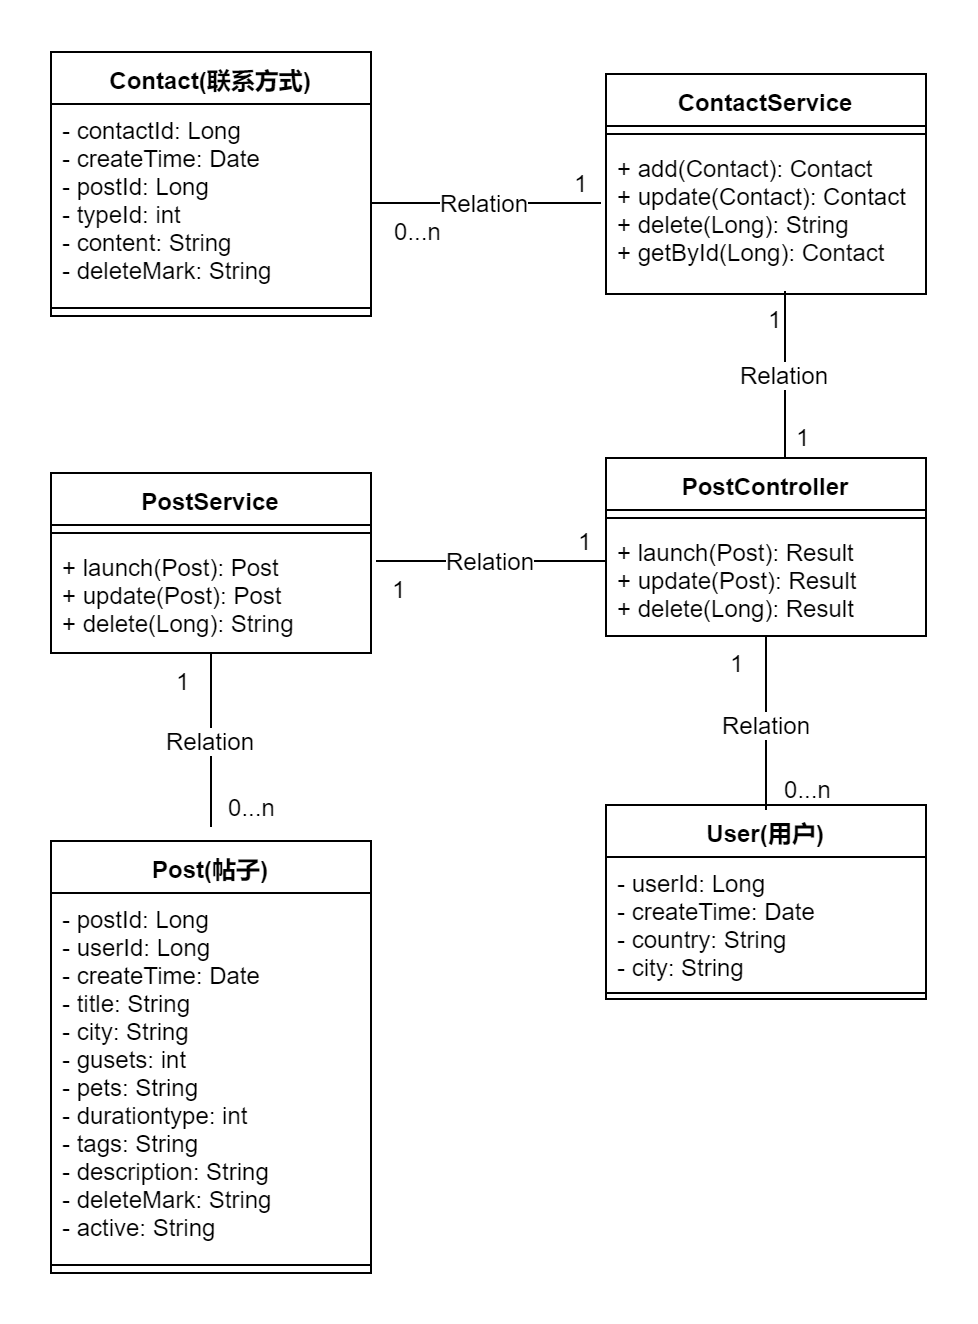
\includegraphics[width=1\textwidth]{ch5/DeletePost.jpg}
    \caption{删除房源}\label{fig:DeletePost}
    \vspace{\baselineskip} % 表示图与正文空一行
\end{figure}
\section{发布新闻}
发布新闻主要为编辑者的操作,该模块要求编辑者填写新闻的详细信息,包括新闻标题,新闻内容,关键词等,如果是引用的别的网站的新闻则需要注明引用链接,
新闻模块是所有用户均能观看。新闻需要进行审核才能发布。涉及到的实体类有用户类(User),新闻类(News),审核类(AuditLog)。具体方法都在NewsController中进行调用。
\begin{figure}[htbp]
    \centering
    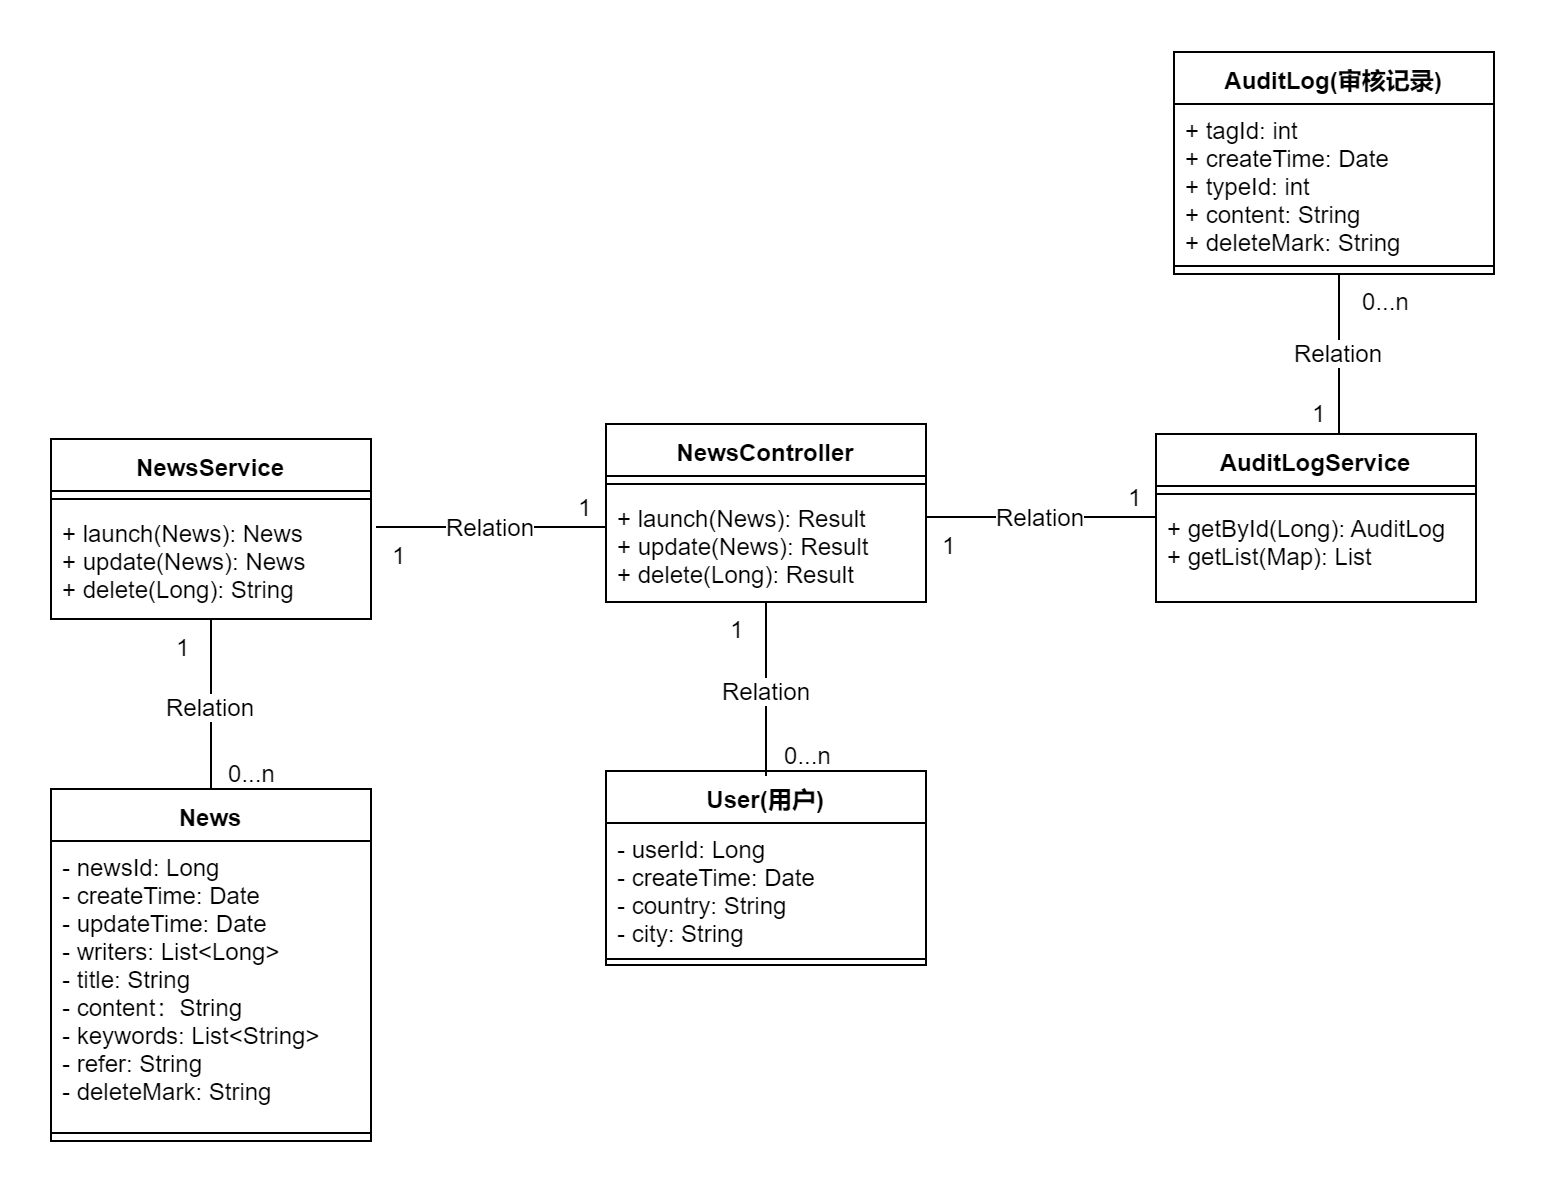
\includegraphics[width=1\textwidth]{ch5/LaunchNews.jpg}
    \caption{发布新闻}\label{fig:LaunchNews}
    \vspace{\baselineskip} % 表示图与正文空一行
\end{figure}
\section{修改新闻}
编辑者可以查看自己发布的新闻,然后进行修改,比如修改内容,修改标题等等,修改后需要审核才能发布。具体的方法还是在NewsController中调用。
\begin{figure}[htbp]
    \centering
    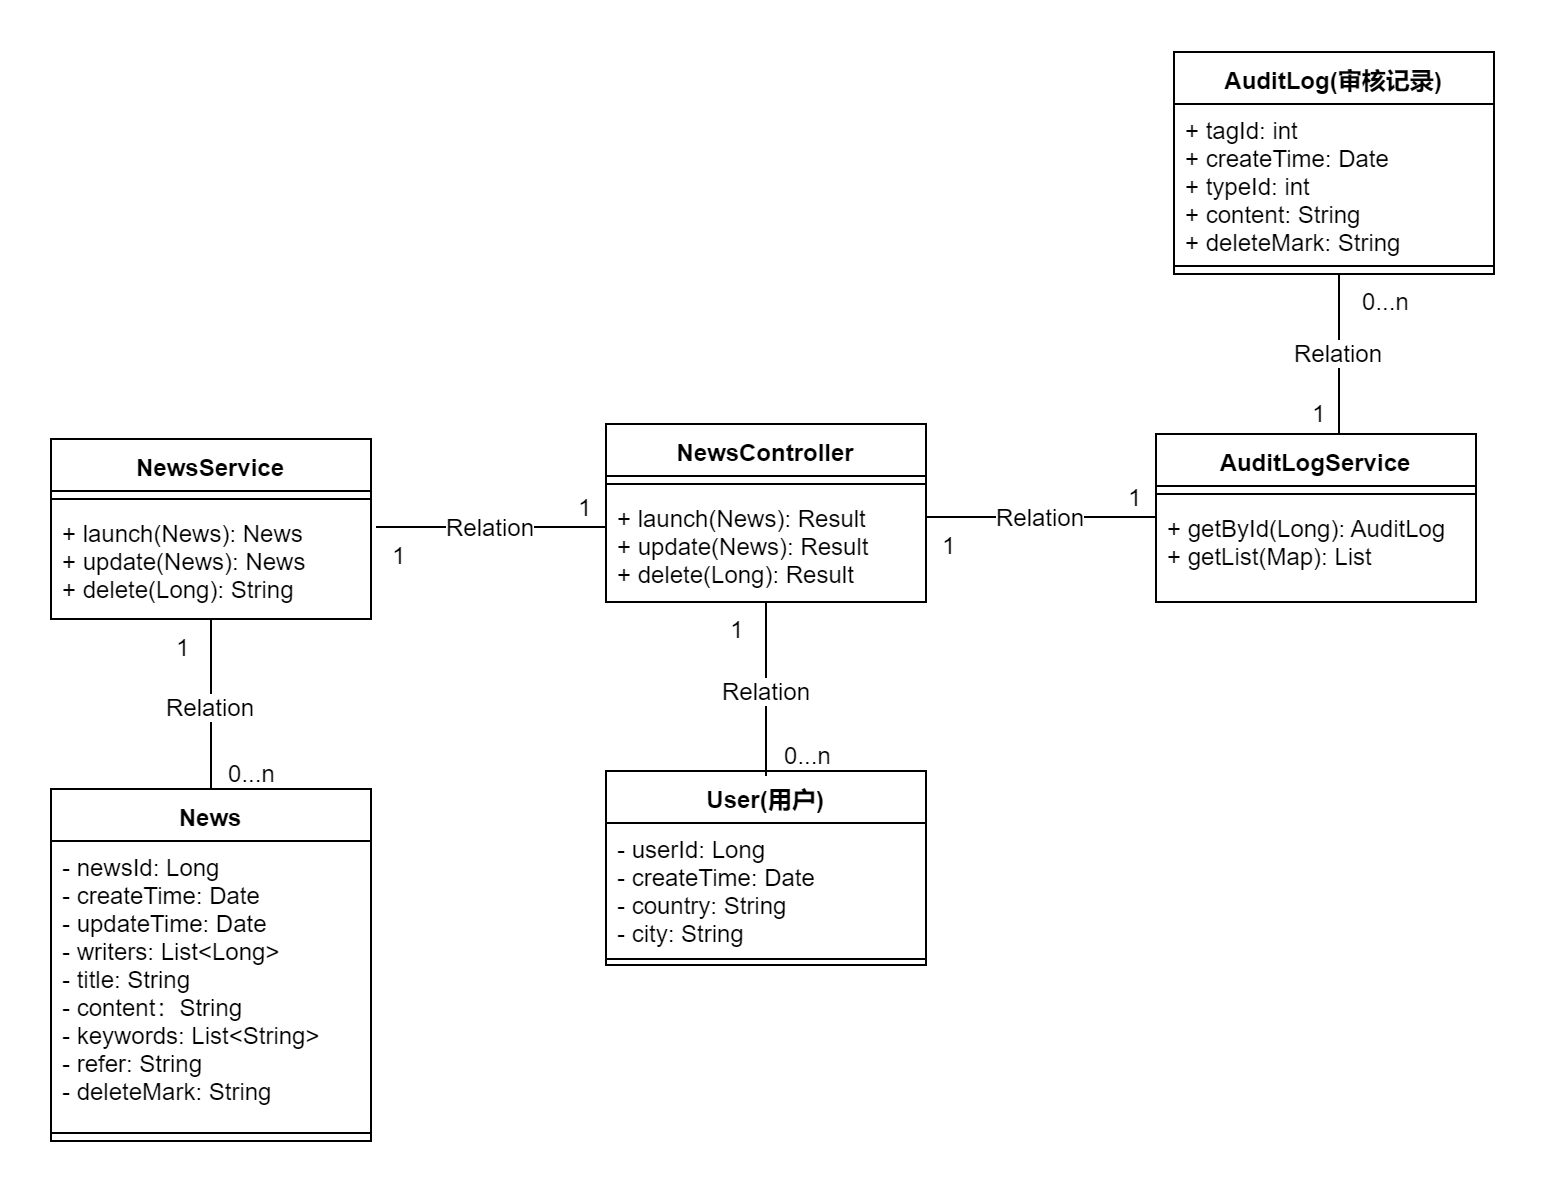
\includegraphics[width=1\textwidth]{ch5/LaunchNews.jpg}
    \caption{修改新闻}\label{fig:UpdateNews}
    \vspace{\baselineskip} % 表示图与正文空一行
\end{figure}
\section{删除新闻}
管理员可以查看发布的新闻,然后删除操作,具体的方法是在NewsController中调用。
\begin{figure}[htbp]
    \centering
    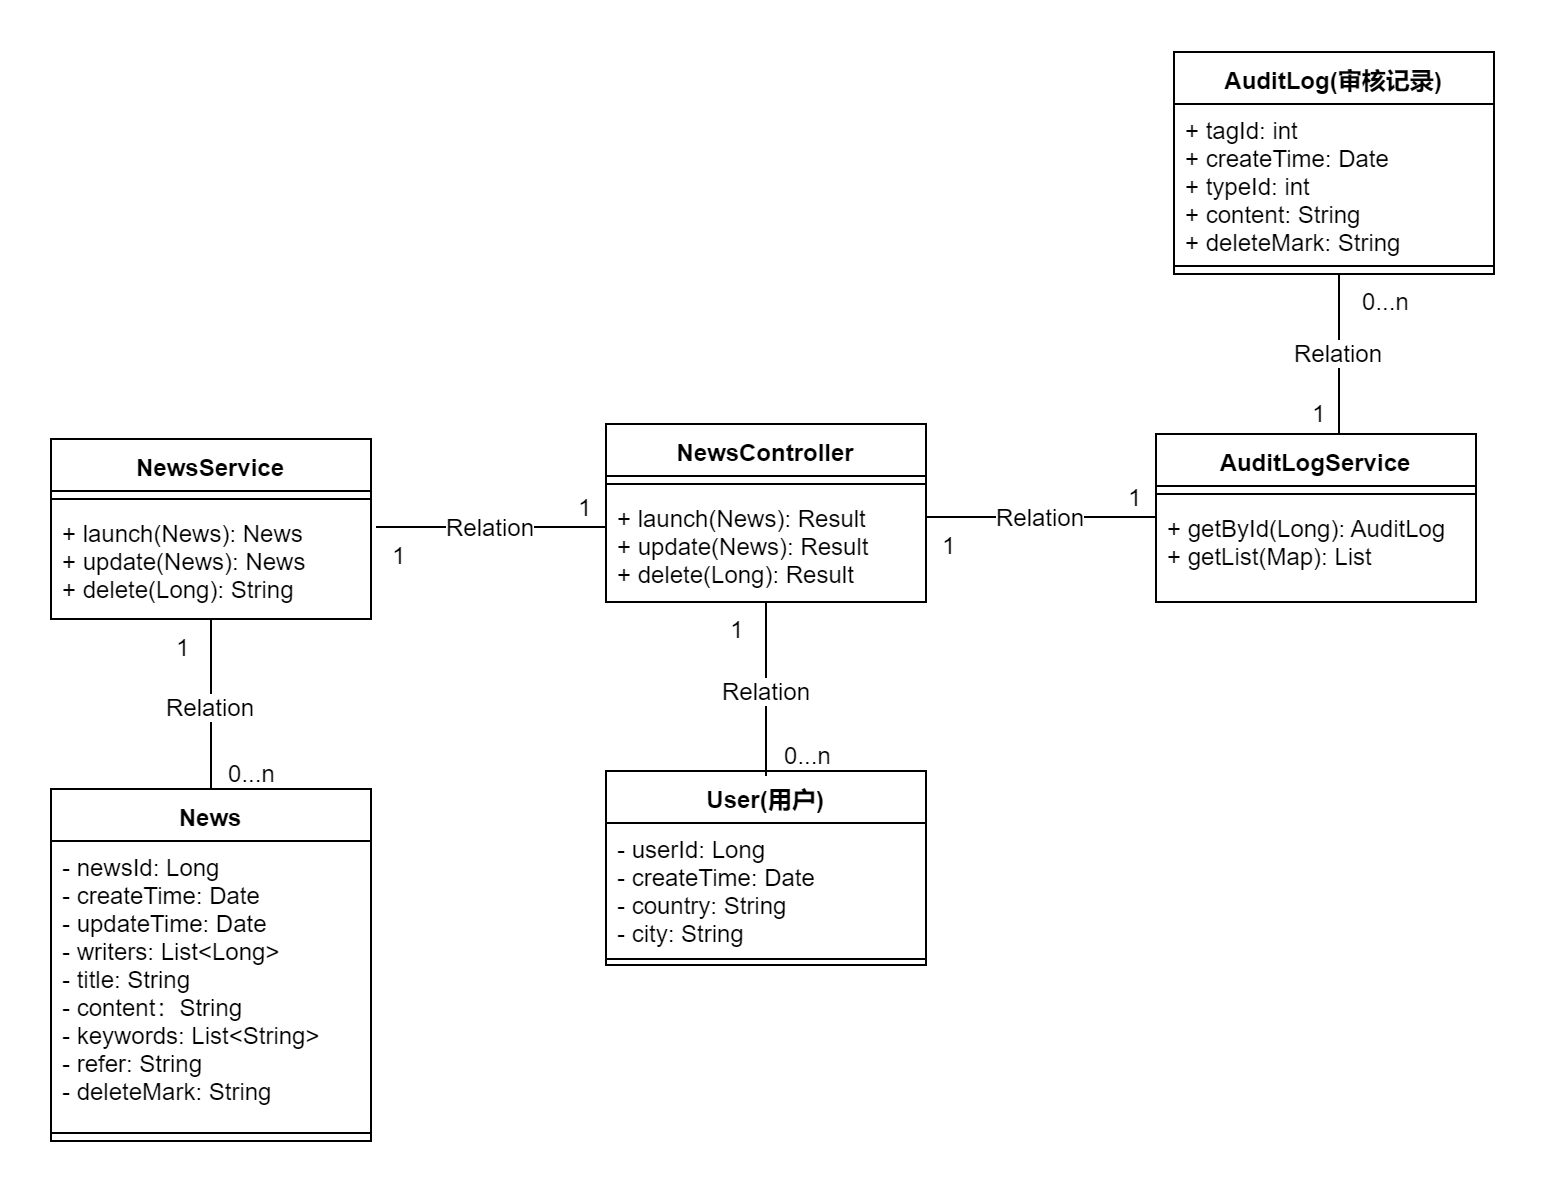
\includegraphics[width=1\textwidth]{ch5/LaunchNews.jpg}
    \caption{删除新闻}\label{fig:DeleteNews}
    \vspace{\baselineskip} % 表示图与正文空一行
\end{figure}
\section{举报}
所有用户都可以对新闻或者房源进行举报,举报需要填写举报理由,然后会由管理员进行审核,管理员会和被举报的用户进行交涉,若举报信息属实则下架发布信息。
涉及到的实体类有用户类(User),举报类(Report),审核类(AuditLog)。具体方法均在ReportController中进行调用。
\begin{figure}[htbp]
    \centering
    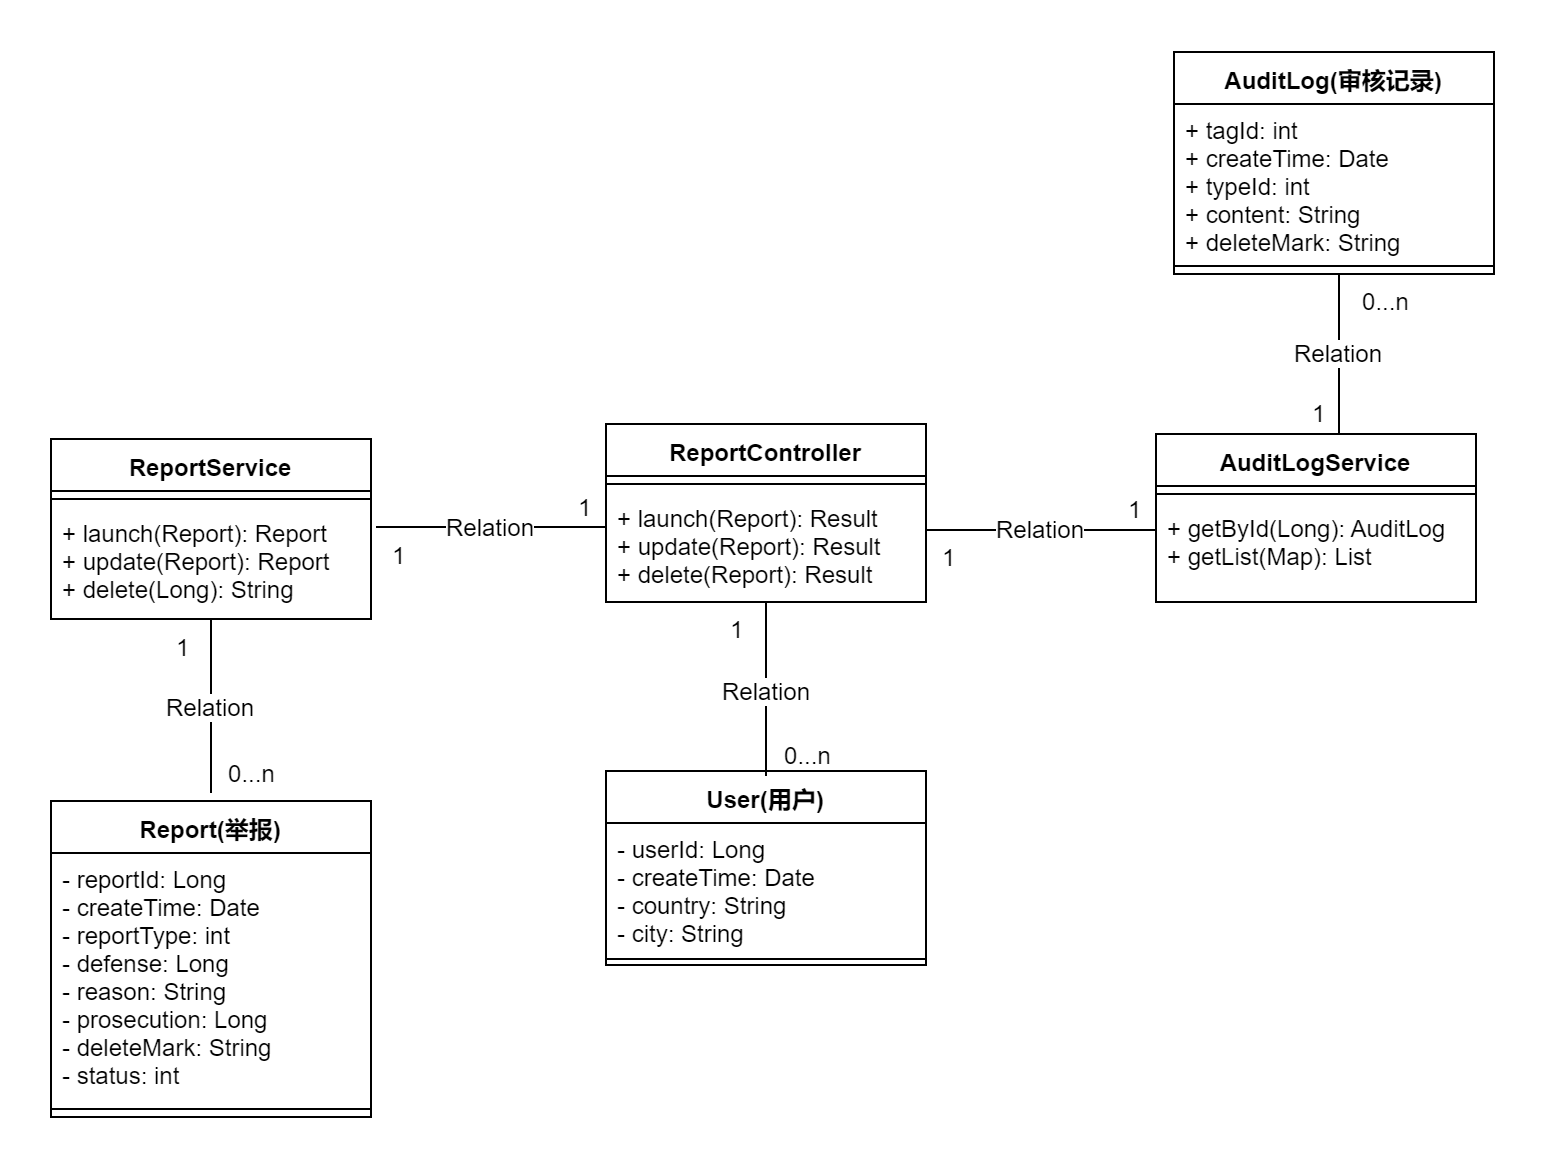
\includegraphics[width=1\textwidth]{ch5/Report.jpg}
    \caption{举报}\label{fig:Report}
    \vspace{\baselineskip} % 表示图与正文空一行
\end{figure}
\section{举报审核}
管理员对用户的举报进行审核,审核需要填写审核结果、审核信息,同时,还需要给涉及到的用户反馈审核结果,及通过系统通知反馈给举报人和被举报人,若举报人为
游客,则不予反馈。涉及到的实体类有用户类(User),举报类(Report),审核类(AuditLog),消息类(Message)。具体方法在AuditLogController中调用。
\begin{figure}[htbp]
    \centering
    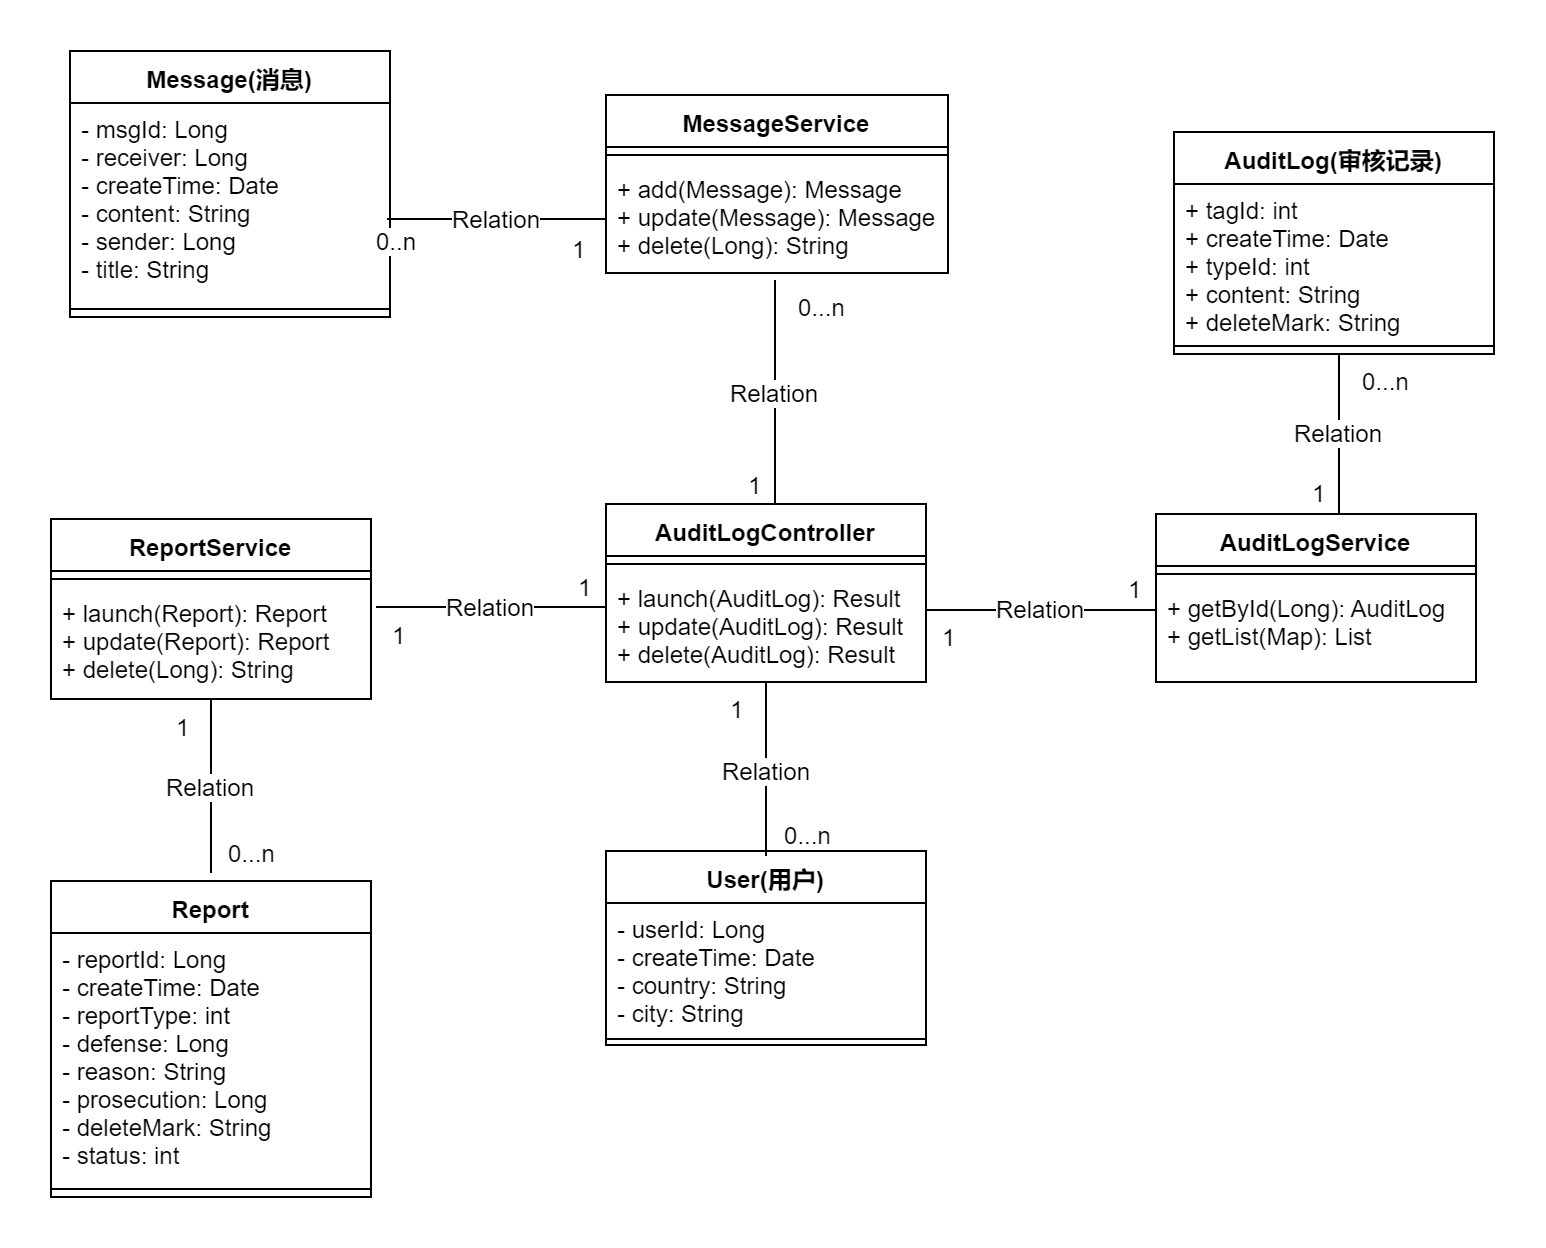
\includegraphics[width=1\textwidth]{ch5/AuditReport.jpg}
    \caption{举报审核}\label{fig:AuditReport}
    \vspace{\baselineskip} % 表示图与正文空一行
\end{figure}
\section{系统通知}
管理员通过消息的方式对用户进行系统通知,系统通知可以对全体用户广播,也可以针对于个别用户,管理员需要选择通知人群,填写通知内容。涉及到的实体类
有用户类(User),消息类(Message),具体方法在MessageController中调用。
\begin{figure}[htbp]
    \centering
    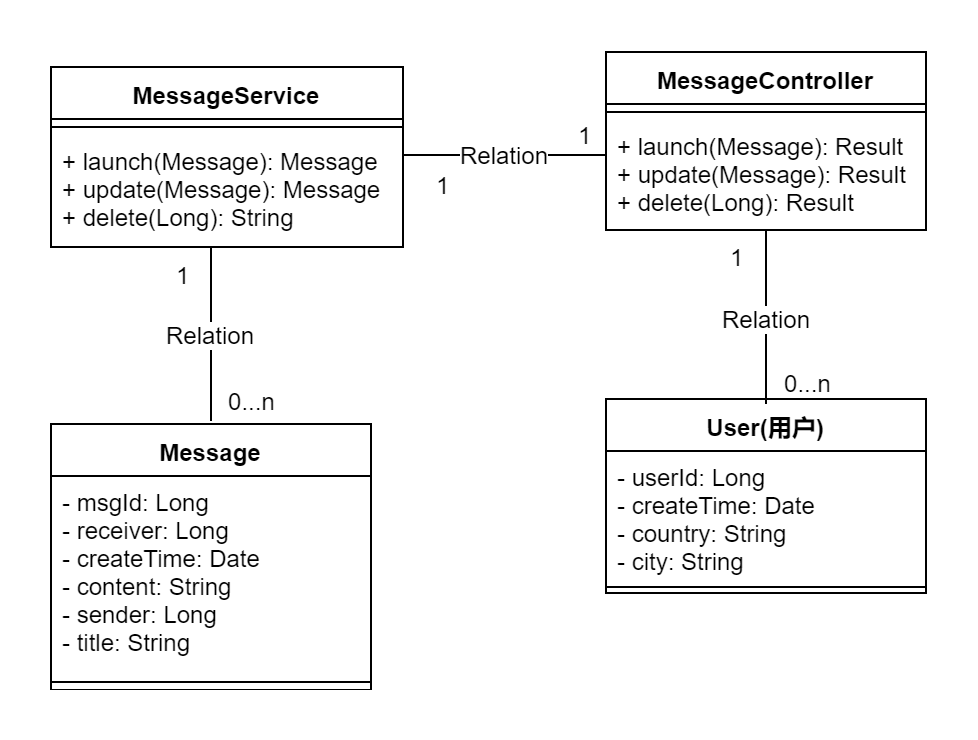
\includegraphics[width=1\textwidth]{ch5/Message.jpg}
    \caption{系统通知}\label{fig:Message}
    \vspace{\baselineskip} % 表示图与正文空一行
\end{figure}
\section{用户管理}
管理员可以通过后台对用户进行管理,包括用户封禁、用户查询、用户赋权、剥夺用户权限等操作,该模块的作用主要是对于用户权限的操作,涉及到的实体类有
用户类(User),角色类(Role),权限类(Permission)。涉及到的方法在UserController中进行调用。
\begin{figure}[htbp]
    \centering
    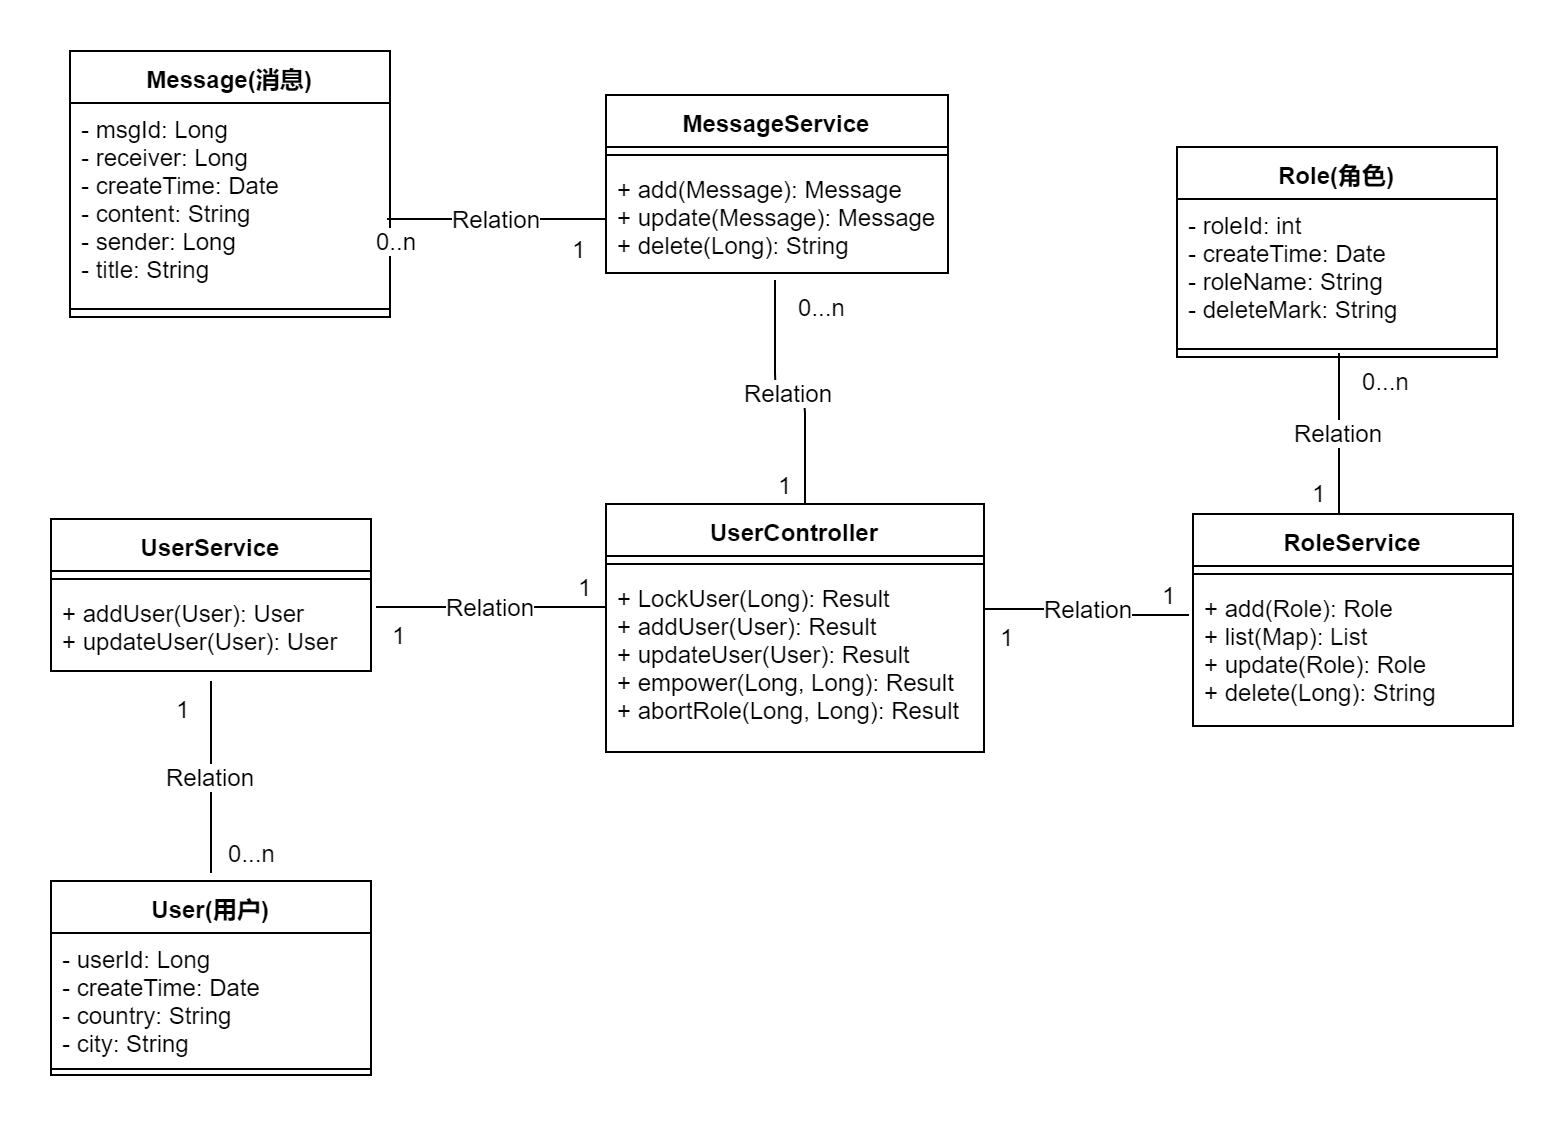
\includegraphics[width=1\textwidth]{ch5/UserManager.jpg}
    \caption{用户管理}\label{fig:UserManager}
    \vspace{\baselineskip} % 表示图与正文空一行
\end{figure}
\section{角色管理}
管理员可以通过后台对角色进行管理,包括删除角色,新增角色、角色赋权、剥夺角色权限等,该模块的作用主要是对于角色权限的操作,涉及到的实体类有
角色类(Role),权限类(Permission)。涉及到的方法在RoleController中进行调用。
\begin{figure}[htbp]
    \centering
    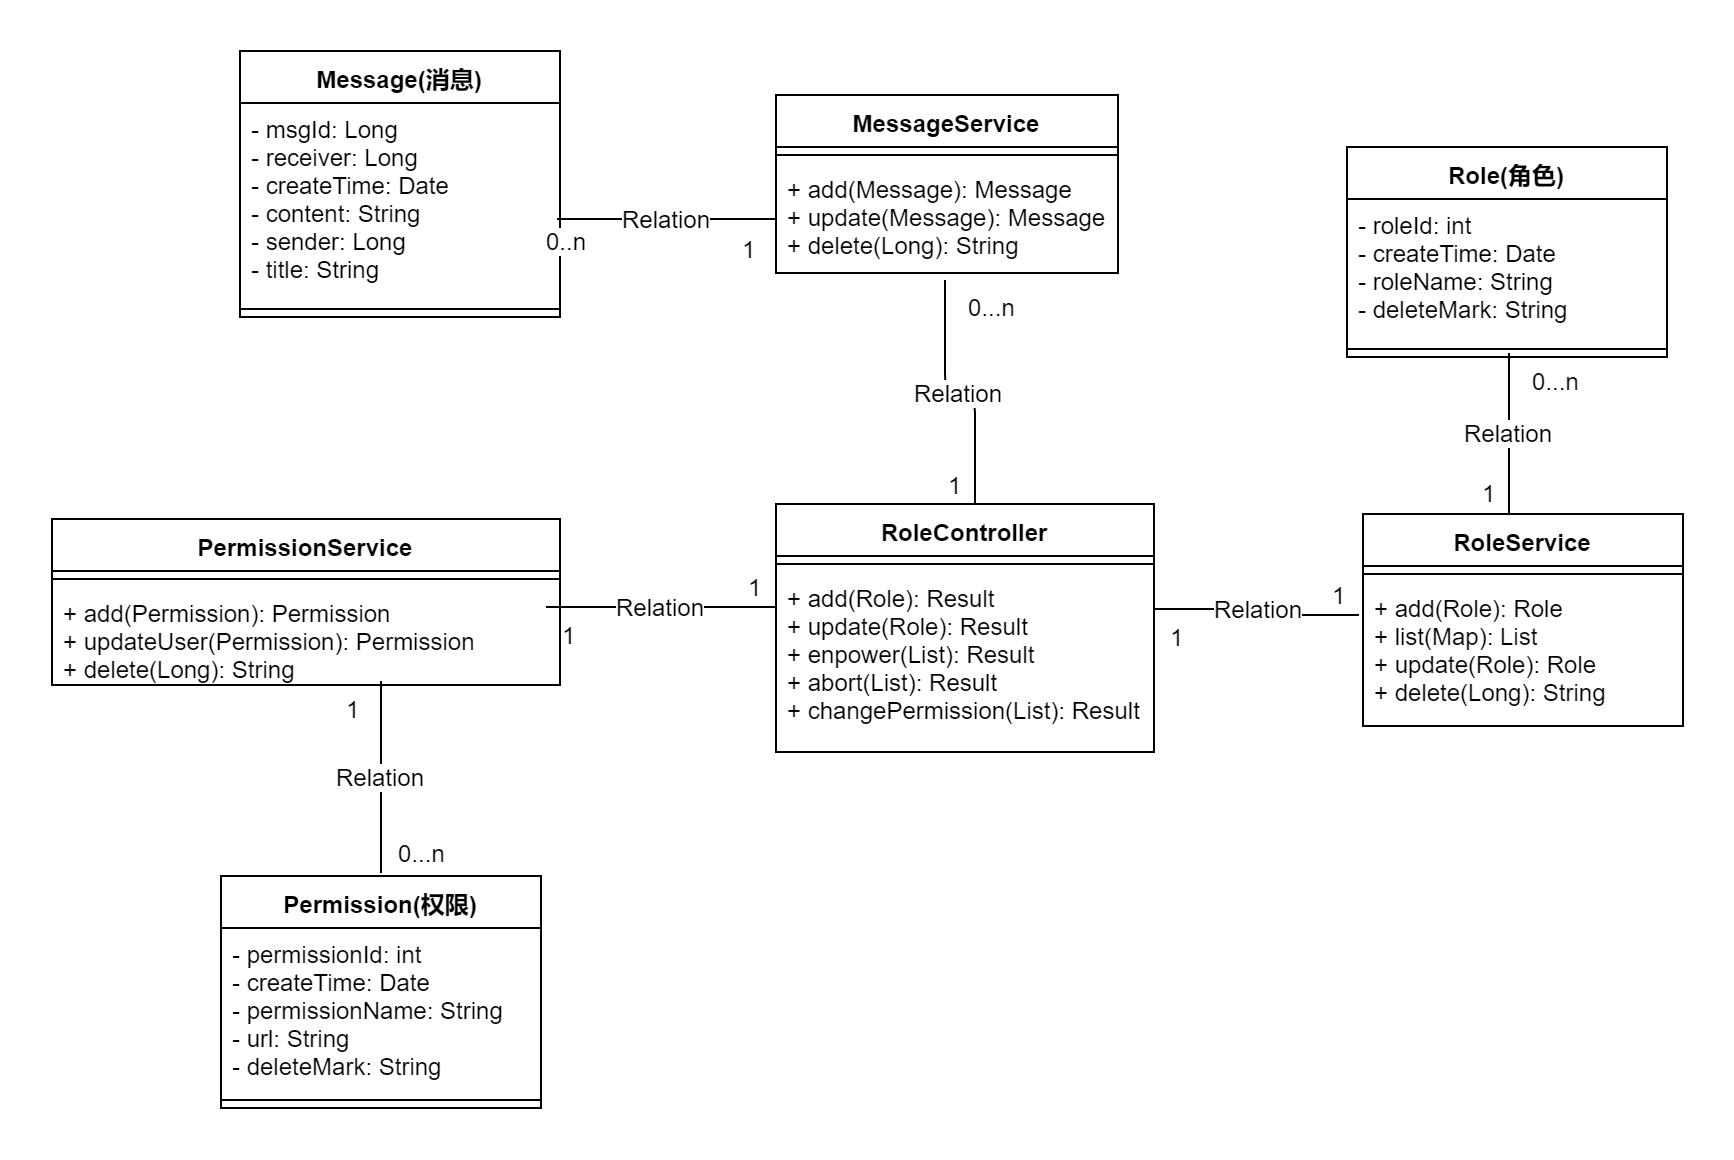
\includegraphics[width=1\textwidth]{ch5/RoleManager.jpg}
    \caption{角色管理}\label{fig:RoleManager}
    \vspace{\baselineskip} % 表示图与正文空一行
\end{figure}
\section{权限管理}
管理员可以通过后台对权限进行管理,包括删除权限,新增权限等,涉及到的实体类为权限类(Permission),方法均在PermissionController中调用。
\begin{figure}[htbp]
    \centering
    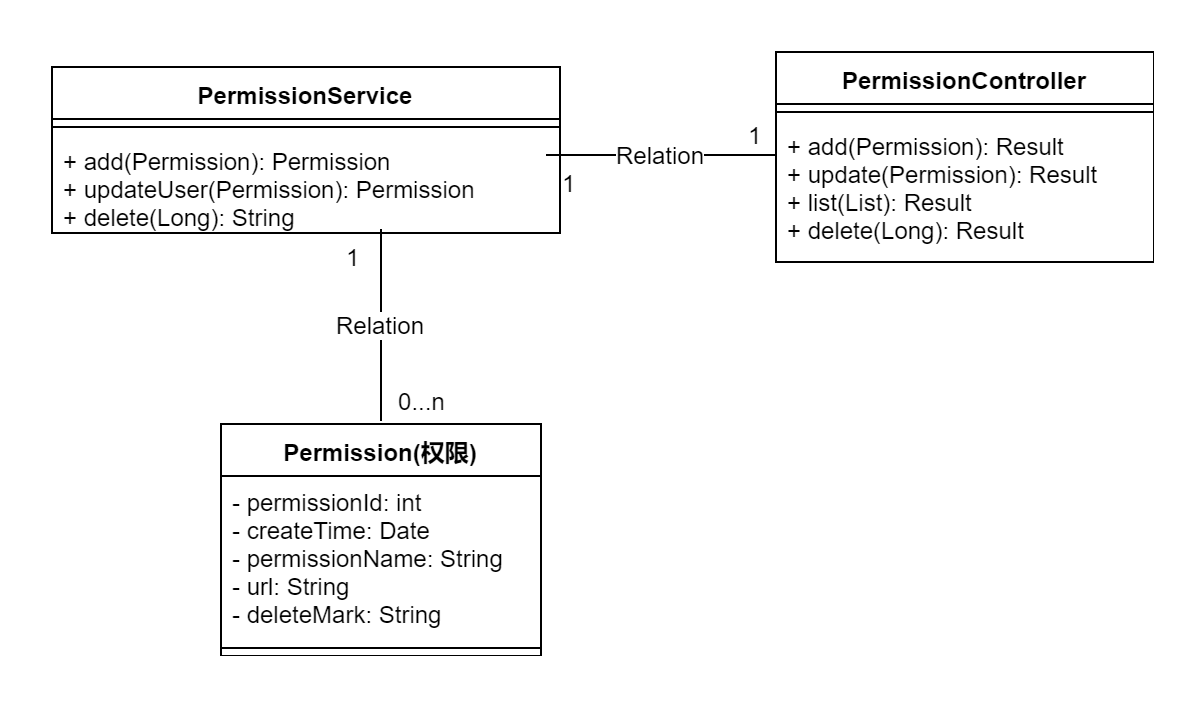
\includegraphics[width=1\textwidth]{ch5/PermissionManager.jpg}
    \caption{权限管理}\label{fig:PermissionManager}
    \vspace{\baselineskip} % 表示图与正文空一行
\end{figure}


\chapter{详细设计}
前几章设计了系统的框架、层次、业务对象等方面,本章将对系统进行详尽的设计,包括数据库的设计,主要流程的设计等。
\section{数据库设计}
本系统使用的是MySQL数据库,由于系统框架为微服务框架,所以本章将分模块为设计各自模块的数据库表。同时,为了提高查询速度,便于开发,
所有的数据表均不会设置外键,也没有触发器,全靠后端上层逻辑保证数据的完整性。后期为提高查询速度会设计索引和视图。
\subsection{UserService用户模块}
用户模块的数据表主要设计用户基本信息、角色信息、权限信息等,一方面是为用户登录认证授权服务,另一方面是为管理员进行用户管理服务。权限管理方面采用的是RBAC的数据表设计,即将权限信息分为5个表,
用户信息表、角色信息表、权限信息表、用户角色表和权限角色表。
\subsubsection{User角色表}
\begin{enumerate}
    \item 表结构
    \begin{table}[htbp]
        \centering
        \scalebox{0.6}{
        \begin{tabular}{|l|l|l|l|l|}
        \hline
        字段名          & 字段类型         & 字段描述   & 初始值              & 约束                        \\ \hline
        USER\_ID     & Long         & 用户唯一约束 &                  & PK,AUTO\_INCREMENT        \\ \hline
        CREATE\_TIME & Date         & 创建时间   & CURRENTTIMESTAMP & NULL DEFAULT CURRENTSTAMP \\ \hline
        COUNTRY      & VARCHAR(100) & 国家     &                  &                           \\ \hline
        CITY         & VARCHAR(200) & 城市     &                  &                           \\ \hline
        \end{tabular}
        }
        \end{table}
    \item 建表语句\\
        CREATE TABLE(\\
            USER\_ID INT(64) PRIMARY KEY AUTO\_INCREMENT,\\
            CREATE\_TIME TIMESTAMP NULL DEFAULT CURRENTTIMESTAMP,\\
            COUNTRY VARCHAR(100),\\
            CITY VARCHAR(200)\\
        )
    \end{enumerate}

\subsubsection{USER\_AUTH用户认证表}
本系统支持第三方登录,所以每个用户对应多个登陆凭证和密码,比如邮箱、手机号等。本表记录的就是用户和对应的登陆方式,包括用户ID、登陆账号、登陆密码、登陆方式等。
\begin{enumerate}
    \item 表结构
    \begin{table}[htbp]
        \centering
        \scalebox{0.6}{
        \begin{tabular}{|l|l|l|l|l|}
        \hline
        \hline
        字段名            & 字段类型         & 字段描述   & 初始值              & 约束                        \\ \hline
        AUTH\_ID       & Long         & 用户唯一约束 &                  & PK,AUTO\_INCREMENT        \\ \hline
        CREATE\_TIME   & Date         & 创建时间   & CURRENTTIMESTAMP & NULL DEFAULT CURRENTSTAMP \\ \hline
        USER\_ID       & Long         & 关联用户标识 &                  & NOT NULL                  \\ \hline
        IDENTITY\_TYPE & int          & 登录类别标识 &                  & NOT NULL                  \\ \hline
        IDENTIFIER     & VARCHAR(50)  & 身份唯一标识 &                  & NOT NULL                  \\ \hline
        CREDENTIAL     & VARCHAR(100) & 登陆验证   &                  & NOT NULL                  \\ \hline
        \end{tabular}
        }
        \end{table}
    \item 建表语句\\
        CREATE TABLE(\\
            AUTH\_ID INT(64) PRIMARY KEY AUTO\_INCREMENT,\\
            USER\_ID INT(64) PRIMARY KEY AUTO\_INCREMENT,\\
            CREATE\_TIME TIMESTAMP NULL DEFAULT CURRENTTIMESTAMP,\\
            IDENTITY\_TYPE INT NOT NULL,\\
            IDENTIFIER VARCHAR(50) NOT NULL,\\
            CREDENTIAL VARCHAR(100) NOT NULL\\
        )
    \end{enumerate}

\subsubsection{DICT\_ROLE角色表}
为了便于权限管理,根据RBAC设计,将多个权限抽象出来,封装在一个角色中。角色表和用户表是多对多的关系,即一个用户可以拥有多个角色,一个角色也可以被多个角色拥有。
\begin{enumerate}
    \item 表结构
    \begin{table}[htbp]
        \centering
        \scalebox{0.6}{
        \begin{tabular}{|l|l|l|l|l|}
        \hline
        \hline
        字段名            & 字段类型         & 字段描述   & 初始值              & 约束                        \\ \hline
        ROLE\_ID     & Long         & 角色唯一约束 &                  & PK,AUTO\_INCREMENT        \\ \hline
        CREATE\_TIME & Date         & 创建时间   & CURRENTTIMESTAMP & NULL DEFAULT CURRENTSTAMP \\ \hline
        ROLE\_NAME   & VARCHAR(30)  & 角色名称   &                  & NOT NULL                  \\ \hline
        DELETE\_MARK & VARCHAR(3)   & 删除标识   & NO               & NULL DEFAULT 'NO'         \\ \hline
        \end{tabular}
        }
        \end{table}
    \item 建表语句\\
        CREATE TABLE(\\
            ROLE\_ID INT(64) PRIMARY KEY AUTO\_INCREMENT,\\
            CREATE\_TIME TIMESTAMP NULL DEFAULT CURRENTTIMESTAMP,\\
            ROLE\_NAME VARCHAR(30) NOT NULL,\\
            DELETE\_MARK VARCHAR(3) NULL DEFAULT 'NO'\\
        )
    \end{enumerate}

\subsubsection{DICT\_PERMISSION权限表}
权限表记载了系统中的所有权限,本系统中的权限值对应的是请求路径,即本系统的权限控制是基于URL的。角色表和权限表是多对多的关系,即一个角色拥有多个权限,一个权限也可以被多个角色拥有。
\begin{enumerate}
    \item 表结构
    \begin{table}[htbp]
        \centering
        \scalebox{0.6}{
        \begin{tabular}{|l|l|l|l|l|}
        \hline
        \hline
        字段名            & 字段类型         & 字段描述   & 初始值              & 约束                        \\ \hline
        PERMISSION\_ID & Long         & 权限唯一约束 &                  & PK,AUTO\_INCREMENT        \\ \hline
        CREATE\_TIME   & Date         & 创建时间   & CURRENTTIMESTAMP & NULL DEFAULT CURRENTSTAMP \\ \hline
        PERMISSION     & VARCHAR(30)  & 权限名称   &                  & NOT NULL                  \\ \hline
        DELETE\_MARK   & VARCHAR(3)   & 删除标识   & NO               & NULL DEFAULT 'NO'         \\ \hline
        \end{tabular}
        }
        \end{table}
    \item 建表语句\\
        CREATE TABLE(\\
            PERMISSION\_ID INT(64) PRIMARY KEY AUTO\_INCREMENT,\\
            CREATE\_TIME TIMESTAMP NULL DEFAULT CURRENTTIMESTAMP,\\
            PERMISSION\_NAME VARCHAR(30) NOT NULL,\\
            DELETE\_MARK VARCHAR(3) NULL DEFAULT 'NO'\\
        )
    \end{enumerate}

\subsubsection{DICT\_USER\_ROLE用户角色表}
此表为用户和角色的关联关系表,将用户id和角色id建立关联,从而可以知道用户对应的角色。
\begin{enumerate}
    \item 表结构
    \begin{table}[htbp]
        \centering
        \scalebox{0.6}{
        \begin{tabular}{|l|l|l|l|l|}
        \hline
        \hline
        字段名            & 字段类型         & 字段描述   & 初始值              & 约束                        \\ \hline
        ROLE\_ID     & Long         & 角色唯一约束 &                  & PK,AUTO\_INCREMENT        \\ \hline
        USER\_ID     & Long         & 用户唯一约束 &                &NOT NULL \\ \hline
        CREATE\_TIME & Date         & 创建时间   & CURRENTTIMESTAMP & NULL DEFAULT CURRENTSTAMP \\ \hline
        LOCK\_MARK   & VARCHAR(3)   & 冻结标识   & NO               & NULL DEFAULT 'NO'         \\ \hline
        DELETE\_MARK & VARCHAR(3)   & 删除标识   & NO               & NULL DEFAULT 'NO'         \\ \hline
        \end{tabular}
        }
        \end{table}
    \item 建表语句\\
        CREATE TABLE(\\
            ROLE\_ID INT(64) PRIMARY KEY AUTO\_INCREMENT,\\
            USER\_ID INT(64) NOT NULL, \\
            CREATE\_TIME TIMESTAMP NULL DEFAULT CURRENTTIMESTAMP,\\
            LOCK\_MARK VARCHAR(3) NULL DEFAULT 'NO', \\            
            DELETE\_MARK VARCHAR(3) NULL DEFAULT 'NO'\\
        )
    \end{enumerate}

\subsubsection{DICT\_ROLE\_PERMISSION角色权限表}
此表为角色和权限的关联关系表,将角色id和权限id建立关联,从而可以获取角色对应的权限。
\begin{enumerate}
    \item 表结构
    \begin{table}[htbp]
        \centering
        \scalebox{0.6}{
        \begin{tabular}{|l|l|l|l|l|}
        \hline
        \hline
        字段名            & 字段类型         & 字段描述   & 初始值              & 约束                        \\ \hline
        ROLE\_ID     & Long         & 角色唯一约束 &                  & PK,AUTO\_INCREMENT        \\ \hline
        PERMISSION\_ID     & Long         & 权限唯一约束 &                &NOT NULL \\ \hline
        CREATE\_TIME & Date         & 创建时间   & CURRENTTIMESTAMP & NULL DEFAULT CURRENTSTAMP \\ \hline
        LOCK\_MARK   & VARCHAR(3)   & 冻结标识   & NO               & NULL DEFAULT 'NO'         \\ \hline
        DELETE\_MARK & VARCHAR(3)   & 删除标识   & NO               & NULL DEFAULT 'NO'         \\ \hline
        \end{tabular}
        }
        \end{table}
    \item 建表语句\\
        CREATE TABLE(\\
            ROLE\_ID INT(64) PRIMARY KEY AUTO\_INCREMENT,\\
            PERMISSION\_ID INT(64) NOT NULL, \\
            CREATE\_TIME TIMESTAMP NULL DEFAULT CURRENTTIMESTAMP,\\
            LOCK\_MARK VARCHAR(3) NULL DEFAULT 'NO', \\            
            DELETE\_MARK VARCHAR(3) NULL DEFAULT 'NO'\\
        )
    \end{enumerate}

\subsubsection{表格关系}
该模块共涉及了6张表,下图~\ref{fig:USER-ER}~为6张表的关系。
\begin{figure}[htbp]
    \centering
    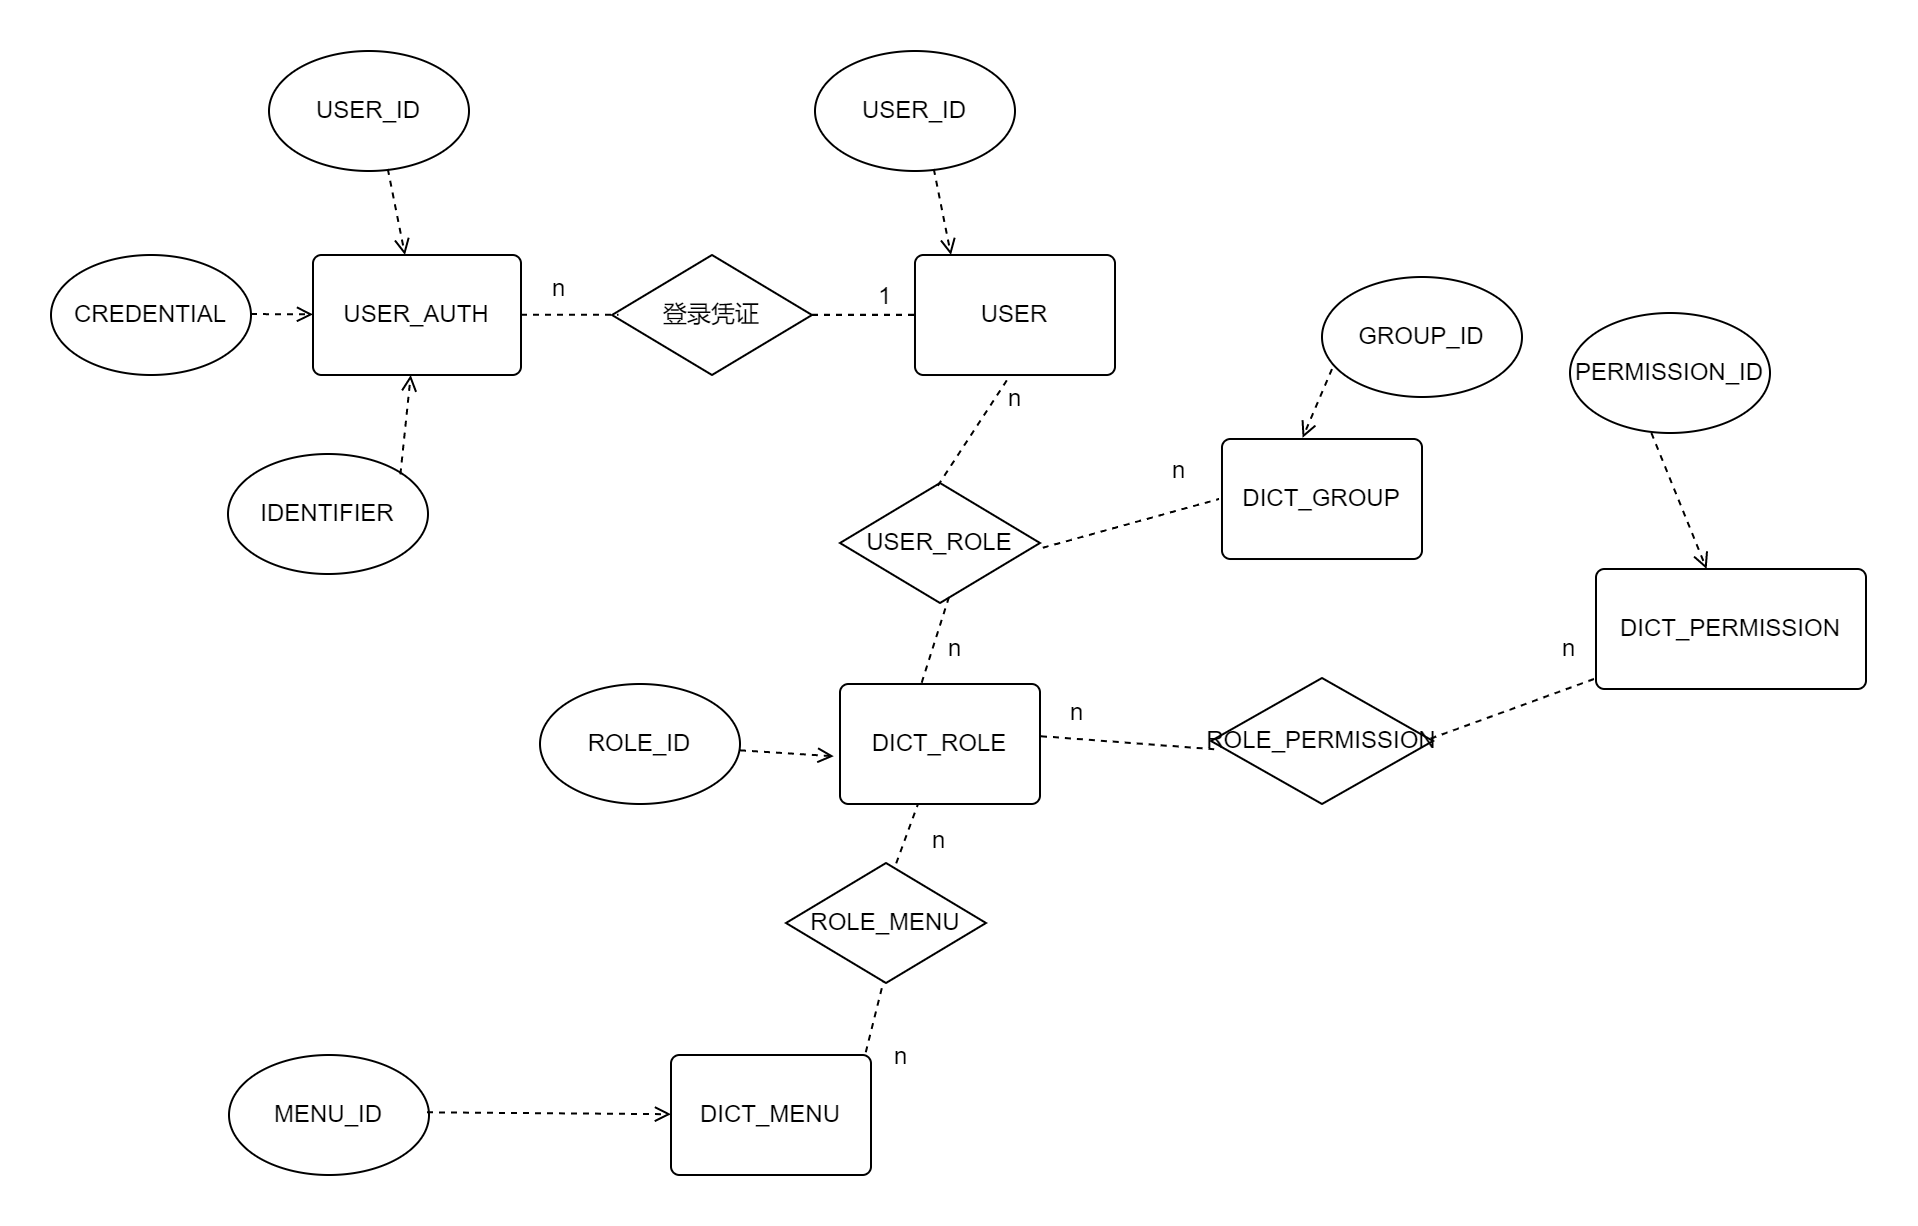
\includegraphics[width=\textwidth]{ch7/USER-ER.jpg}
    \caption{用户管理模块ER图}\label{fig:USER-ER}
    \vspace{\baselineskip} % 表示图与正文空一行
\end{figure}

\subsection{HouseService房源模块}
房源模块主要涉及帖子基本信息、房主联系方式、帖子标签等等和房源帖子相关的数据表。为了功能的扩展性,我们会设置多个字典表,便于功能的增删改,比如标签表的设置是为了方便房源标签的及时增删。
\subsubsection{POST帖子表}
房源帖子包含了帖子的基本信息,比如房源地址、是否允许宠物、房源标签、房源描述等等。
\begin{enumerate}
    \item 表结构
    \begin{table}[htbp]
        \centering
        \scalebox{0.6}{
        \begin{tabular}{|l|l|l|l|l|}
        \hline
        \hline
        字段名            & 字段类型         & 字段描述   & 初始值              & 约束                        \\ \hline
        POST\_ID     & Long         & 帖子唯一约束    &                   & PK,AUTO\_INCREMENT               \\ \hline
        CREATE\_TIME & Date         & 创建时间      & CURRENTTIMESTAMP  & NULL DEFAULT CURRENTSTAMP        \\ \hline
        USER\_ID     & Long         & 关联用户标识    &                   & NOT NULL                         \\ \hline
        DELETE\_MARK & VARCHAR(3)   & 删除标识      & NO                & NULL DEFAULT 'NO'                \\ \hline
        TITLE        & VARCHAR(200) & 标题        & WE CAN OFFER HELP & NULL DEFAULT 'WE CAN OFFER HELP' \\ \hline
        CITY         & VARCHAR(200) & 城市(市,省,国) &                   & NOT NULL                         \\ \hline
        GUESTS       & int          & 人数        & 1                 & NULL DEFAULT 1                   \\ \hline
        PETS         & VARCHAR(3)   & 是否允许宠物    & NO                & NULL DEFAULT 'NO'                \\ \hline
        DURATIONTYPE & int          & 时长类型      & 1                 & NULL DEFAULT 1                   \\ \hline
        TAGS         & VARCHAR(200) & 标签组        &                   &                                  \\ \hline
        ACTIVE       & VARCHAR(3)   & 有效表示      & YES               & NULL DEFAULT 'YES'               \\ \hline
        DESCRIPTION  & VARCHAR(500) & 住所描述
        \end{tabular}
        }
        \end{table}
    \item 建表语句\\
        CREATE TABLE(\\
            POST\_ID INT(64) PRIMARY KEY AUTO\_INCREMENT,\\
            USER\_ID INT(64) NOT NULL, \\
            CREATE\_TIME TIMESTAMP NULL DEFAULT CURRENTTIMESTAMP,\\
            DELETE\_MARK VARCHAR(3) NULL DEFAULT 'NO',\\
            TITLE VARCHAR(200) NULL DEFAULT 'WE CAN OFFER HEPL',\\
            CITY VARCHAR(200) NOT NULL,\\
            GUESTS INT NULL DEFAULT 1,\\
            PETS VARCHAR(3) NULL DEFAULT 'NO',\\
            DURATIONTYPE INT NULL DEFAULT 1,\\
            TAGS VARCHAR(200),\\
            DESCRIPTION VARCHAR(500),\\
            ACTIVE VARCHAR(3) NULL DEFAULT 'YES'\\
        )
    \end{enumerate}

\subsubsection{CONTACT联系方式表}
此表记录了房源帖上具体的联系方式,为了便于联系方式的增删改,我们将联系方式独立出来形成一张数据表,以减少耦合度。表中主要记录了对应的帖子,以及基本的联系信息。
\begin{enumerate}
    \item 表结构
    \begin{table}[htbp]
        \centering
        \scalebox{0.6}{
        \begin{tabular}{|l|l|l|l|l|}
        \hline
        \hline
        字段名            & 字段类型         & 字段描述   & 初始值              & 约束                        \\ \hline
        CONTACT\_ID  & Long         & 唯一约束     &                  & PK,AUTO\_INCREMENT        \\ \hline
        CREATE\_TIME & Date         & 创建时间     & CURRENTTIMESTAMP & NULL DEFAULT CURRENTSTAMP \\ \hline
        POST\_ID     & Long         & 关联关联标识   &                  & NOT NULL                  \\ \hline
        DELETE\_MARK & VARCHAR(3)   & 删除标识     & NO               & NULL DEFAULT 'NO'         \\ \hline
        CONTENT      & VARCHAR(200) & 联系途径     &                  & NOT NULL                  \\ \hline
        TYPE\_ID     & int          & 联系方式类别标识 &                  & NOT NULL                  \\ \hline
        \end{tabular}
        }
        \end{table}
    \item 建表语句\\
        CREATE TABLE(\\
            CONTACT\_ID INT(64) PRIMARY KEY AUTO\_INCREMENT,\\
            POST\_ID INT(64) NOT NULL,\\
            CREATE\_TIME TIMESTAMP NULL DEFAULT CURRENTTIMESTAMP,\\
            DELETE\_MARK VARCHAR(3) NULL DEFAULT 'NO',\\
            CONTENT VARCHAR(200) NOT NULL,\\
            TYPE\_ID INT NOT NULL\\
        )
    \end{enumerate}

\subsubsection{DICT\_CONTACT\_TYPE联系方式类别表}
此表记录了房源帖上那些联系方式的类型,为了后续可以便于直接增加联系方式类型,比如现阶段支持电话和邮箱,一段时间后想增加微信功能,独立出一个类别较容易扩展。
\begin{enumerate}
    \item 表结构
    \begin{table}[htbp]
        \centering
        \scalebox{0.6}{
        \begin{tabular}{|l|l|l|l|l|}
        \hline
        \hline
        字段名            & 字段类型         & 字段描述   & 初始值              & 约束                        \\ \hline
        TYPE\_ID      & int          & 唯一约束     &                  & PK,AUTO\_INCREMENT        \\ \hline
        CREATE\_TIME  & Date         & 创建时间     & CURRENTTIMESTAMP & NULL DEFAULT CURRENTSTAMP \\ \hline
        CONTACT\_NAME & VARCHAR(30)  & 联系方式     &                  & NOT NULL                  \\ \hline
        DELETE\_MARK  & VARCHAR(3)   & 删除标识     & NO               & NULL DEFAULT 'NO'         \\ \hline
        \end{tabular}
        }
        \end{table}
    \item 建表语句\\
        CREATE TABLE(\\
            TYPE\_ID INT PRIMARY KEY AUTO\_INCREMENT,\\
            CREATE\_TIME TIMESTAMP NULL DEFAULT CURRENTTIMESTAMP,\\
            DELETE\_MARK VARCHAR(3) NULL DEFAULT 'NO',\\
            CONTACT\_NAME VARCHAR(30) NOT NULL\\
        )
    \end{enumerate}

\subsubsection{DICT\_TAG标签表}
此表记录了房源帖子上具体的标签,比如标签的类型,标签的内容等。比如说,一个房源帖子的标签为“拥有药物资源,类别为救助”等等。
\begin{enumerate}
    \item 表结构
    \begin{table}[htbp]
        \centering
        \scalebox{0.6}{
        \begin{tabular}{|l|l|l|l|l|}
        \hline
        \hline
        字段名            & 字段类型         & 字段描述   & 初始值              & 约束                        \\ \hline
        TAG\_ID      & int          & 唯一约束     &                  & PK,AUTO\_INCREMENT        \\ \hline
        CREATE\_TIME & Date         & 创建时间     & CURRENTTIMESTAMP & NULL DEFAULT CURRENTSTAMP \\ \hline
        TYPE\_ID     & int          & 标签类别     &                  & NOT NULL                  \\ \hline
        DELETE\_MARK & VARCHAR(3)   & 删除标识     & NO               & NULL DEFAULT 'NO'         \\ \hline
        CONTENT      & VARCHAR(200) & 标签内容     &                  & NOT NULL                  \\ \hline
        \end{tabular}
        }
        \end{table}
    \item 建表语句\\
        CREATE TABLE(\\
            TAG\_ID INT PRIMARY KEY AUTO\_INCREMENT,\\
            CREATE\_TIME TIMESTAMP NULL DEFAULT CURRENTTIMESTAMP,\\
            DELETE\_MARK VARCHAR(3) NULL DEFAULT 'NO',\\
            CONTENT VARCHAR(200) NOT NULL,\\
            TYPE\_ID INT NOT NULL\\
        )
    \end{enumerate}

\subsubsection{DICT\_TAG\_TYPE标签类别表}
每个标签都有对应的类别,这是为了便于管理,也是为了便于扩展,此表记录了标签类别信息,包括类别id、类别内容等。
\begin{enumerate}
    \item 表结构
    \begin{table}[htbp]
        \centering
        \scalebox{0.6}{
        \begin{tabular}{|l|l|l|l|l|}
        \hline
        \hline
        字段名            & 字段类型         & 字段描述   & 初始值              & 约束                        \\ \hline
        TYPE\_ID      & int          & 唯一约束     &                  & PK,AUTO\_INCREMENT        \\ \hline
        CREATE\_TIME  & Date         & 创建时间     & CURRENTTIMESTAMP & NULL DEFAULT CURRENTSTAMP \\ \hline
        TYPE\_NAME    & VARCHAR(50)  & 类别内容     &                  & NOT NULL                  \\ \hline
        DELETE\_MARK  & VARCHAR(3)   & 删除标识     & NO               & NULL DEFAULT 'NO'         \\ \hline
        \end{tabular}
        }
        \end{table}
    \item 建表语句\\
        CREATE TABLE(\\
            TYPE\_ID INT PRIMARY KEY AUTO\_INCREMENT,\\
            CREATE\_TIME TIMESTAMP NULL DEFAULT CURRENTTIMESTAMP,\\
            DELETE\_MARK VARCHAR(3) NULL DEFAULT 'NO',\\
            TYPE\_NAME VARCHAR(50) NOT NULL\\
        )
    \end{enumerate}

\subsubsection{DICT\_DURATION时长类型表}
此表记录了帖子里时长的信息,比如一周、一月、无限期等。
\begin{enumerate}
    \item 表结构
    \begin{table}[htbp]
        \centering
        \scalebox{0.6}{
        \begin{tabular}{|l|l|l|l|l|}
        \hline
        \hline
        字段名            & 字段类型         & 字段描述   & 初始值              & 约束                        \\ \hline
        DURATION\_ID      & int          & 唯一约束     &                  & PK,AUTO\_INCREMENT        \\ \hline
        CREATE\_TIME  & Date         & 创建时间     & CURRENTTIMESTAMP & NULL DEFAULT CURRENTSTAMP \\ \hline
        DURATION    & VARCHAR(50)  & 时长描述     &                  & NOT NULL                  \\ \hline
        DELETE\_MARK  & VARCHAR(3)   & 删除标识     & NO               & NULL DEFAULT 'NO'         \\ \hline
        \end{tabular}
        }
        \end{table}
    \item 建表语句\\
        CREATE TABLE(\\
            DURATION\_ID INT PRIMARY KEY AUTO\_INCREMENT,\\
            CREATE\_TIME TIMESTAMP NULL DEFAULT CURRENTTIMESTAMP,\\
            DELETE\_MARK VARCHAR(3) NULL DEFAULT 'NO',\\
            DURATION VARCHAR(50) NOT NULL\\
        )
    \end{enumerate}


\subsubsection{总体ER图}
本模块的数据表均围绕房源帖子POST展开,下图~\ref{fig:HOUSE-ER}~给出本模块的ER图。
\begin{figure}[htbp]
    \centering
    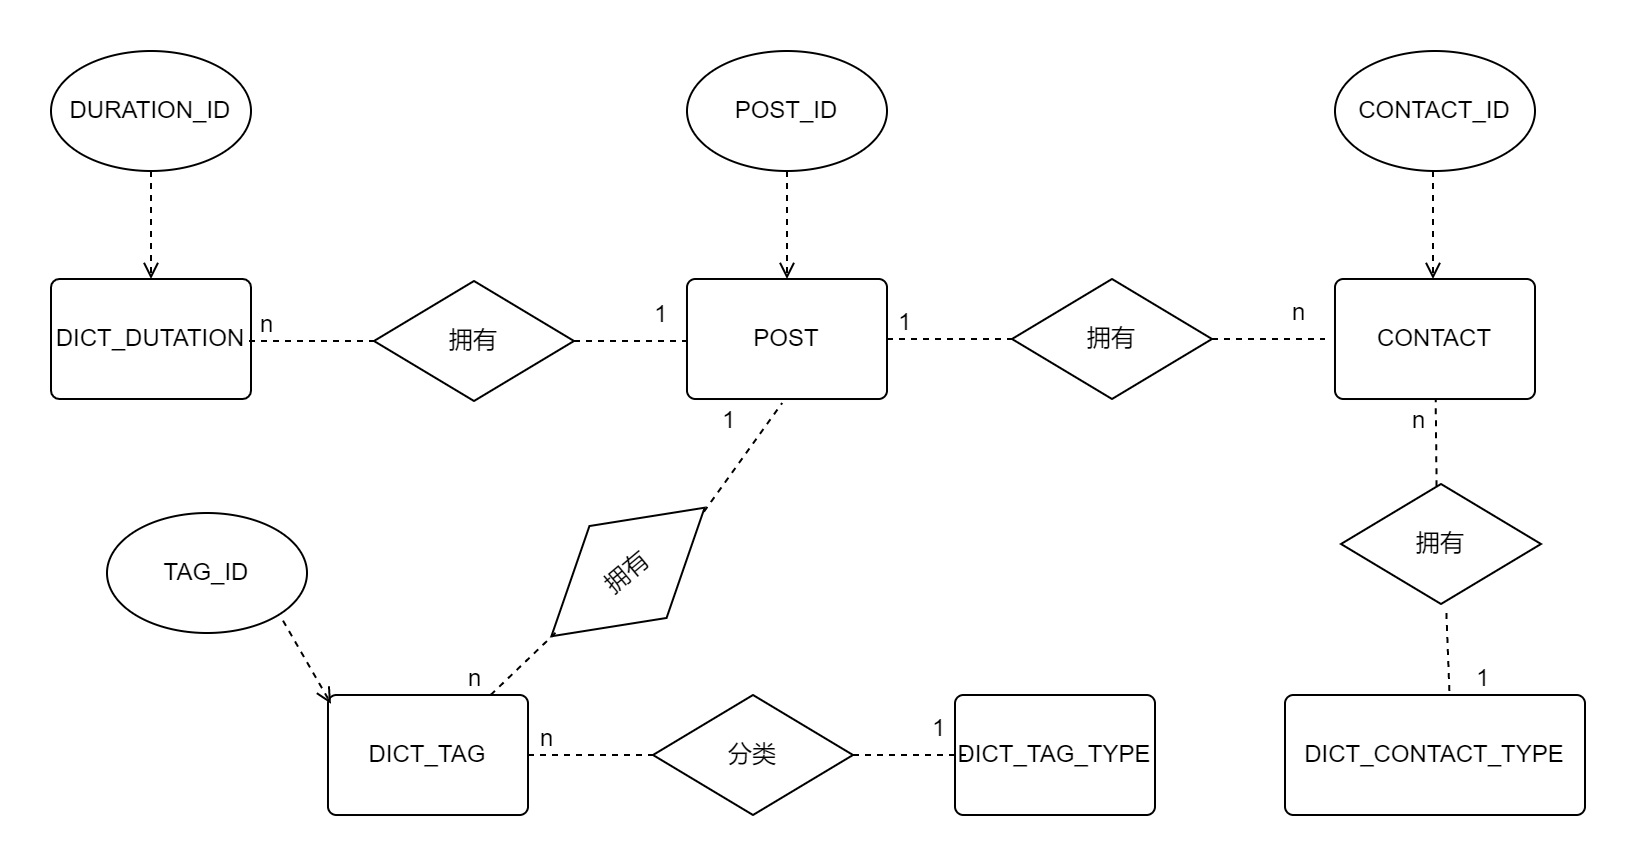
\includegraphics[width=\textwidth]{ch7/HOUSE-ER.jpg}
    \caption{房源管理ER图}\label{fig:HOUSE-ER}
    \vspace{\baselineskip} % 表示图与正文空一行
\end{figure}

\subsection{Report举报模块}
举报模块主要涉及举报基本信息,同时会和其余的模块进行联通,比如用户表、房源帖子表等。
\subsubsection{REPORT举报信息表}
此表记录了举报的基本信息,包括举报内容、举报理由、举报类别、举报人等等。
\begin{enumerate}
    \item 表结构
    \begin{table}[htbp]
        \centering
        \scalebox{0.6}{
        \begin{tabular}{|l|l|l|l|l|}
        \hline
        \hline
        字段名            & 字段类型         & 字段描述   & 初始值              & 约束                        \\ \hline
        REPORT\_ID    & Long         & 唯一约束 &                  & PK,AUTO\_INCREMENT        \\ \hline
        CREATE\_TIME  & Date         & 创建时间 & CURRENTTIMESTAMP & NULL DEFAULT CURRENTSTAMP \\ \hline
        OBJTYPE\_ID    & int          & 举报类型 &                  & NOT NULL                  \\ \hline
        DELETE\_MARK  & VARCHAR(3)   & 删除标识 & NO               & NULL DEFAULT 'NO'         \\ \hline
        DEFENSE       & Long         & 被举报者 &                  & NOT NULL                  \\ \hline
        RESON         & VARCHAR(500) & 举报利用 &                  & NOT NULL                  \\ \hline
        PROSECUTION   & Long         & 举报者  &                  & NOT NULL                  \\ \hline
        AUDIT\_STATUS & int          & 审核状态 & 1                & NULL DEFAULT 1            \\ \hline
        \end{tabular}
        }
        \end{table}
    \item 建表语句\\
        CREATE TABLE(\\
            REPORT\_ID INT(64) PRIMARY KEY AUTO\_INCREMENT,\\
            CREATE\_TIME TIMESTAMP NULL DEFAULT CURRENTTIMESTAMP,\\
            DELETE\_MARK VARCHAR(3) NULL DEFAULT 'NO',\\
            OBJTYPE\_ID INT NOT NULL,\\
            DEFENSE INT(64) NOT NULL,\\
            RESON VARCHAR(500) NOT NULL,\\
            PROSECUTION LONG NOT NULL,\\
            AUDIT\_STATUS INT NULL DEFAULT 1\\
        )
    \end{enumerate}

\subsection{AUDIT模块}
该模块为本系统的审核模块,记录的信息有审核的基本信息、审核类别等,目的是将系统的历次审核记录下来形成日志,便于管理。】
\subsubsection{AUDIT审核表}
此表记录了审核的基本信息,包括审核内容、操作人、操作类型等等。
\begin{enumerate}
    \item 表结构
    \begin{table}[htbp]
        \centering
        \scalebox{0.6}{
        \begin{tabular}{|l|l|l|l|l|}
        \hline
        \hline
        字段名            & 字段类型         & 字段描述   & 初始值              & 约束                        \\ \hline
        AUDIT\_ID      & Long          & 唯一约束     &                  & PK,AUTO\_INCREMENT        \\ \hline
        CREATE\_TIME  & Date         & 创建时间     & CURRENTTIMESTAMP & NULL DEFAULT CURRENTSTAMP \\ \hline
        OBJTYPE\_ID      & int  & 被审核类别     &                  & NOT NULL                  \\ \hline
        DELETE\_MARK  & VARCHAR(3)   & 删除标识     & NO               & NULL DEFAULT 'NO'         \\ \hline
        STATUS        & int  & 审核状态     & 1    & NULL DEFAULT 1 \\ \hline
        OPERATOR      & Long  & 审核人       &      & NOT NULL \\ \hline
        OPER          & int   & 操作        &       & NOT NULL \\ \hline
        MESSAGE       & VARCHAR(200)    &       & \\ \hline
        \end{tabular}
        }
        \end{table}
    \item 建表语句\\
        CREATE TABLE(\\
            AUDIT\_ID INT PRIMARY KEY AUTO\_INCREMENT,\\
            CREATE\_TIME TIMESTAMP NULL DEFAULT CURRENTTIMESTAMP,\\
            DELETE\_MARK VARCHAR(3) NULL DEFAULT 'NO',\\
            OBJTYPE\_ID INT NOT NULL,\\
            STATUS  INT NOT NULL,\\
            OPERATOR LONG NOT NULL,\\
            OPER INT NOT NULL,\\
            MESSAGE VARCHAR(200) \\
        )
    \end{enumerate}

\subsubsection{DICT\_OPER\_TYPE审核类型表}
此表表示所有业务对象的审核类型,包括管理员通过、管理员驳回等,便于管理和扩展。
\begin{enumerate}
    \item 表结构
    \begin{table}[htbp]
        \centering
        \scalebox{0.6}{
        \begin{tabular}{|l|l|l|l|l|}
        \hline
        \hline
        字段名            & 字段类型         & 字段描述   & 初始值              & 约束                        \\ \hline
        OPER\_ID      & int          & 唯一约束     &                  & PK,AUTO\_INCREMENT        \\ \hline
        CREATE\_TIME  & Date         & 创建时间     & CURRENTTIMESTAMP & NULL DEFAULT CURRENTSTAMP \\ \hline
        DELETE\_MARK  & VARCHAR(3)   & 删除标识     & NO               & NULL DEFAULT 'NO'         \\ \hline
        OPER          & VARCHAR(200)   & 操作        &       & NOT NULL \\ \hline
        \end{tabular}
        }
        \end{table}
    \item 建表语句\\
        CREATE TABLE(\\
            OPER\_ID INT PRIMARY KEY AUTO\_INCREMENT,\\
            CREATE\_TIME TIMESTAMP NULL DEFAULT CURRENTTIMESTAMP,\\
            DELETE\_MARK VARCHAR(3) NULL DEFAULT 'NO',\\
            OPER VARCHAR(200) NOT NULL \\
        )
    \end{enumerate}

\subsubsection{总体ER图}
本模块的总体ER图如图~\ref{fig:AUDIT-ER}所示
\begin{figure}[htbp]
    \centering
    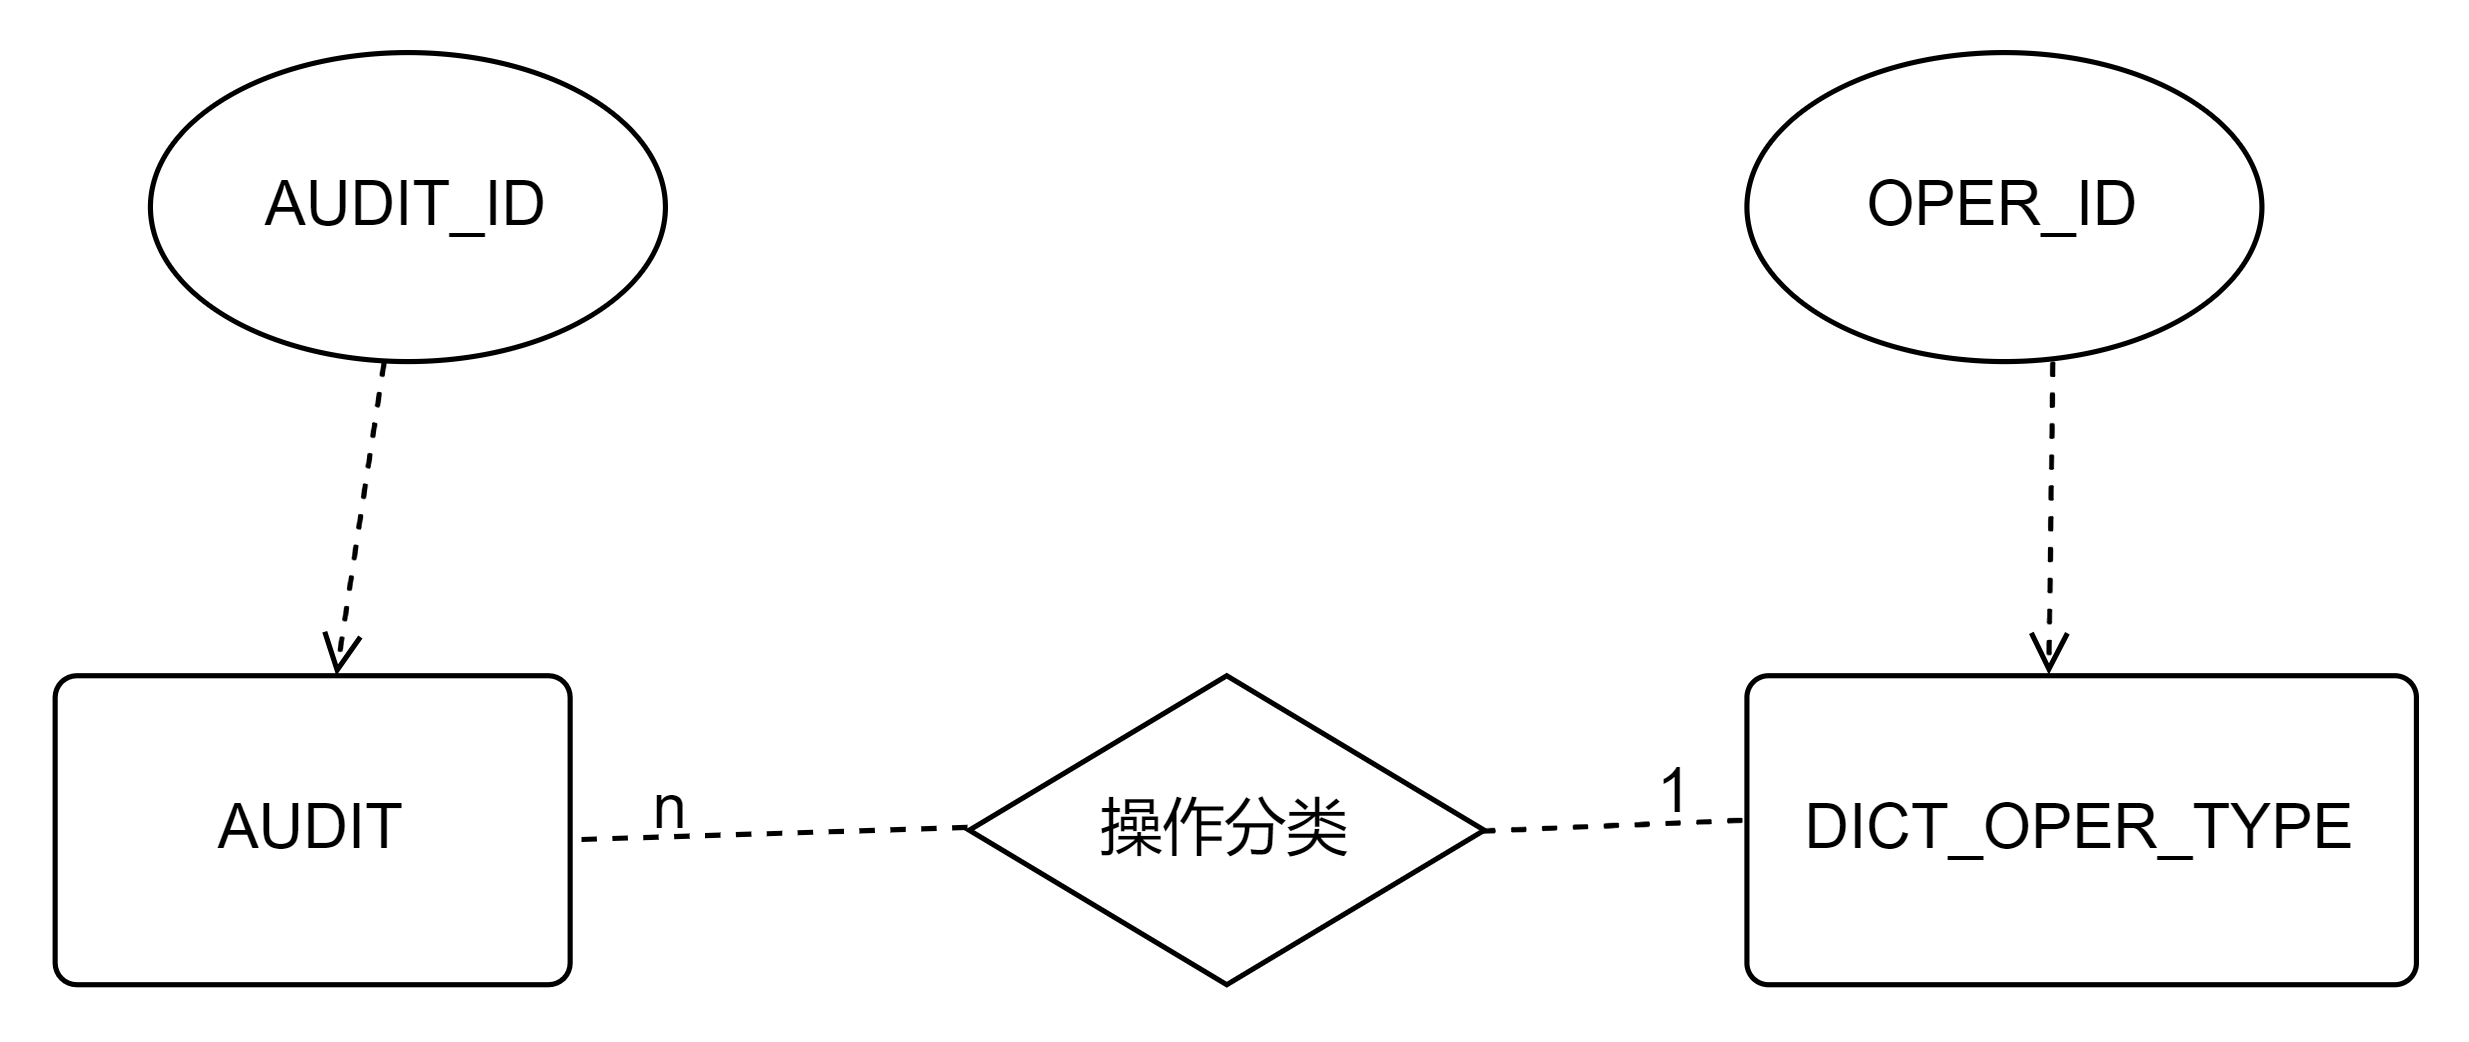
\includegraphics[width=\textwidth]{ch7/AUDIT-ER.jpg}
    \caption{审核模块ER图}\label{fig:AUDIT-ER}
    \vspace{\baselineskip} % 表示图与正文空一行
\end{figure}

\subsection{News模块}
News是新闻模块,涉及到的数据表有新闻基本信息表,新闻内容表,新闻栏目表等。
\subsubsection{NEWS新闻基本信息表}
本表记录了新闻的基本信息,包括新闻的标题、栏目、阅读量等等。
\begin{enumerate}
    \item 表结构
    \begin{table}[htbp]
        \centering
        \scalebox{0.6}{
        \begin{tabular}{|l|l|l|l|l|}
        \hline
        \hline
        字段名            & 字段类型         & 字段描述   & 初始值              & 约束                        \\ \hline
        NEWS\_ID      & Long          & 唯一约束     &                  & PK,AUTO\_INCREMENT        \\ \hline
        CREATE\_TIME  & Date         & 创建时间     & CURRENTTIMESTAMP & NULL DEFAULT CURRENTSTAMP \\ \hline
        DELETE\_MARK  & VARCHAR(3)   & 删除标识     & NO               & NULL DEFAULT 'NO'         \\ \hline
        CATALOGUE     & int          & 栏目        &       & NOT NULL \\ \hline
        TITLE         & VARCHAR(200) & 标题        &       & NOT NULL \\ \hline
        AUTHORS       & VARCHAR(200) & 作者        &       & NOT NULL \\ \hline
        LINK          & VARCHAR(500) & 引用链接    &        &       \\ \hline
        UPDATE\_TIME  & Date         & 修改日期    & CURRENTTIMESTAMP & NULL DEFAULT CURRENTTIMESTAMP \\ \hline
        READ\_NUM     & int          & 阅读量      & 0      & NULL DEFAULT 0 \\ \hline
        \end{tabular}
        }
        \end{table}
    \item 建表语句\\
        CREATE TABLE(\\
            NEWS\_ID INT PRIMARY KEY AUTO\_INCREMENT,\\
            CREATE\_TIME TIMESTAMP NULL DEFAULT CURRENTTIMESTAMP,\\
            DELETE\_MARK VARCHAR(3) NULL DEFAULT 'NO',\\
            CATALOGUE INT NOT NULL ,\\
            TITLE VATCHAR(200) NOT NULL,\\
            AUTHORS VARCHAR(200) NOT NULL,\\
            LINK VARCHAR(200) ,\\
            UPDATE\_TIME TIMESTAMP NULL DEFAULT CURRENTTIMESTAMP,\\
            READ\_NUM INT NULL DEFAULT 0\\
        )
    \end{enumerate}

\subsubsection{NEWS\_PIC新闻图片表}
本表记录了新闻信息中的图片信息,表中保存了图片的链接地址、大小、文件名等信息。
\begin{enumerate}
    \item 表结构
    \begin{table}[htbp]
        \centering
        \scalebox{0.6}{
        \begin{tabular}{|l|l|l|l|l|}
        \hline
        \hline
        字段名            & 字段类型         & 字段描述   & 初始值              & 约束                        \\ \hline
        PIC\_ID      & Long          & 唯一约束     &                  & PK,AUTO\_INCREMENT        \\ \hline
        NEWS\_ID      & Long         & 新闻标识     &                  & NOT NULL \\ \hline
        CREATE\_TIME  & Date         & 创建时间     & CURRENTTIMESTAMP & NULL DEFAULT CURRENTSTAMP \\ \hline
        DELETE\_MARK  & VARCHAR(3)   & 删除标识     & NO               & NULL DEFAULT 'NO'         \\ \hline
        PIC\_NAME     & VARCHAR(100)          & 图片名称        &       & NOT NULL \\ \hline
        FILE\_NAME    & VARCHAR(200) & 文件名        &       & NOT NULL \\ \hline
        FILE\_SIZE    & int          & 大小        &       & NOT NULL \\ \hline
        PIC\_DES          & VARCHAR(500) & 描述    &        &        \\ \hline
        FILE\_PATH     & VARCHAR(200)    & 目录      &       & NOT NULL \\ \hline
        \end{tabular}
        }
        \end{table}
    \item 建表语句\\
        CREATE TABLE(\\
            PIC\_ID INT(64) PRIMARY KEY AUTO\_INCREMENT,\\
            NEW\_ID INT(64) NOT NULL,\\
            CREATE\_TIME TIMESTAMP NULL DEFAULT CURRENTTIMESTAMP,\\
            DELETE\_MARK VARCHAR(3) NULL DEFAULT 'NO',\\
            PIC\_NAME VARCHAR(100) NOT NULL ,\\
            FILE\_NAME VATCHAR(200) NOT NULL,\\
            FILE\_SIZE INT NOT NULL,\\
            PIC\_DES VARCHAR(500) ,\\
            FILE\_PATH VARCHAR(200) NOT NULL\\
        )
    \end{enumerate}

\subsubsection{NEWS\_CONTENT新闻文本表}
此表记录了新闻的文本信息,本系统的文本系统拟定使用MarkDown格式,表中记录了对应的新闻,文本文件的位置等。
\begin{enumerate}
    \item 表结构
    \begin{table}[htbp]
        \centering
        \scalebox{0.6}{
        \begin{tabular}{|l|l|l|l|l|}
        \hline
        \hline
        字段名            & 字段类型         & 字段描述   & 初始值              & 约束                        \\ \hline
        CONTENT\_ID      & Long          & 唯一约束     &                  & PK,AUTO\_INCREMENT        \\ \hline
        NEWS\_ID      & Long         & 新闻标识     &                  & NOT NULL \\ \hline
        CREATE\_TIME  & Date         & 创建时间     & CURRENTTIMESTAMP & NULL DEFAULT CURRENTSTAMP \\ \hline
        DELETE\_MARK  & VARCHAR(3)   & 删除标识     & NO               & NULL DEFAULT 'NO'         \\ \hline
        FILE\_NAME    & VARCHAR(200) & 文件名        &       & NOT NULL \\ \hline
        FILE\_SIZE    & int          & 大小        &       & NOT NULL \\ \hline
        FILE\_PATH     & VARCHAR(200)    & 目录      &       & NOT NULL \\ \hline
        \end{tabular}
        }
        \end{table}
    \item 建表语句\\
        CREATE TABLE(\\
            CONTENT\_ID INT(64) PRIMARY KEY AUTO\_INCREMENT,\\
            NEW\_ID INT(64) NOT NULL,\\
            CREATE\_TIME TIMESTAMP NULL DEFAULT CURRENTTIMESTAMP,\\
            DELETE\_MARK VARCHAR(3) NULL DEFAULT 'NO',\\
            FILE\_NAME VATCHAR(200) NOT NULL,\\
            FILE\_SIZE INT NOT NULL,\\
            FILE\_PATH VARCHAR(200) NOT NULL\\
        )
    \end{enumerate}

\subsubsection{DICT\_CATALOGUE新闻栏目类}
此表记录了新闻的栏目集合,包括栏目名称、创建日期等。
\begin{enumerate}
    \item 表结构
    \begin{table}[htbp]
        \centering
        \scalebox{0.6}{
        \begin{tabular}{|l|l|l|l|l|}
        \hline
        \hline
        字段名            & 字段类型         & 字段描述   & 初始值              & 约束                        \\ \hline
        CATALOGUE\_ID      & int          & 唯一约束     &                  & PK,AUTO\_INCREMENT        \\ \hline
        CREATE\_TIME  & Date         & 创建时间     & CURRENTTIMESTAMP & NULL DEFAULT CURRENTSTAMP \\ \hline
        DELETE\_MARK  & VARCHAR(3)   & 删除标识     & NO               & NULL DEFAULT 'NO'         \\ \hline
        CATALOGUE          & VARCHAR(30)   & 栏目        &       & NOT NULL \\ \hline
        \end{tabular}
        }
        \end{table}
    \item 建表语句\\
        CREATE TABLE(\\
            CATALOGUE\_ID INT PRIMARY KEY AUTO\_INCREMENT,\\
            CREATE\_TIME TIMESTAMP NULL DEFAULT CURRENTTIMESTAMP,\\
            DELETE\_MARK VARCHAR(3) NULL DEFAULT 'NO',\\
            CATALOGUE VARCHAR(30) NOT NULL \\
        )
    \end{enumerate}

\subsubsection{总体ER图}
如图~\ref{fig:NEWS-ER}~所示为NEWS模块的总体ER图。
\begin{figure}[htbp]
    \centering
    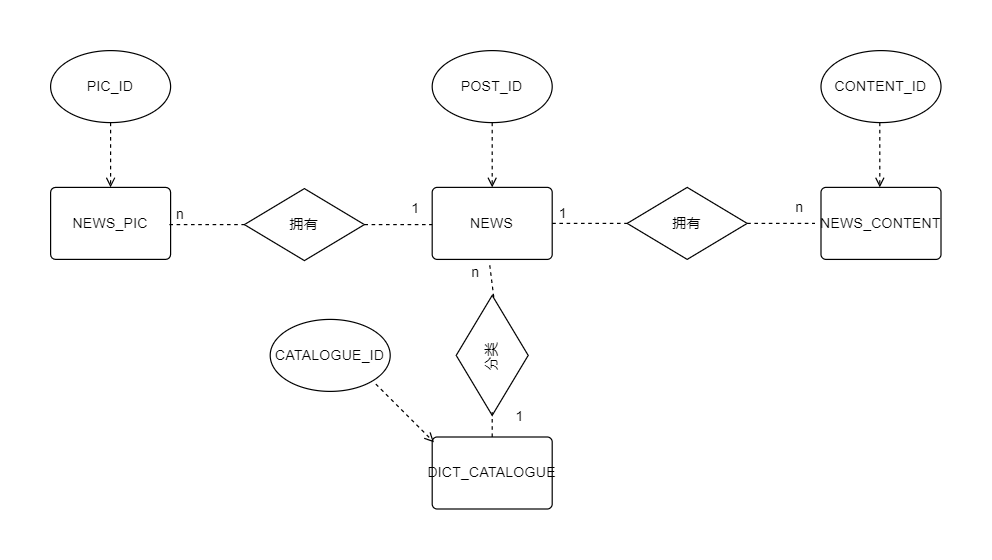
\includegraphics[width=\textwidth]{ch7/NEWS-ER.jpg}
    \caption{新闻模块ER图}\label{fig:NEWS-ER}
    \vspace{\baselineskip} % 表示图与正文空一行
\end{figure}

\subsection{SystemService模块}
该模块为系统管理模块,保存系统相关的数据,比如业务对象类型、系统信息、系统日志等。
\subsubsection{DICT\_OBJTYPE业务对象表}
本表记录了本系统中用到的所有业务对象,并将其进行分类,便于管理和业务对象的扩展。
\begin{enumerate}
    \item 表结构
    \begin{table}[htbp]
        \centering
        \scalebox{0.6}{
        \begin{tabular}{|l|l|l|l|l|}
        \hline
        \hline
        字段名            & 字段类型         & 字段描述   & 初始值              & 约束                        \\ \hline
        OBJTYPE\_ID      & int          & 唯一约束     &                  & PK,AUTO\_INCREMENT        \\ \hline
        CREATE\_TIME  & Date         & 创建时间     & CURRENTTIMESTAMP & NULL DEFAULT CURRENTSTAMP \\ \hline
        DELETE\_MARK  & VARCHAR(3)   & 删除标识     & NO               & NULL DEFAULT 'NO'         \\ \hline
        OBJTYPE          & VARCHAR(100)   & 操作        &       & NOT NULL \\ \hline
        \end{tabular}
        }
        \end{table}
    \item 建表语句\\
        CREATE TABLE(\\
            OBJTYPE\_ID INT PRIMARY KEY AUTO\_INCREMENT,\\
            CREATE\_TIME TIMESTAMP NULL DEFAULT CURRENTTIMESTAMP,\\
            DELETE\_MARK VARCHAR(3) NULL DEFAULT 'NO',\\
            OBJTYPE VARCHAR(200) NOT NULL \\
        )
    \end{enumerate}

\subsubsection{MESSAGE系统信息表}
本表记录了系统消息类,具体包括消息类别、消息人群、操作人等。
\begin{enumerate}
    \item 表结构
    \begin{table}[htbp]
        \centering
        \scalebox{0.6}{
        \begin{tabular}{|l|l|l|l|l|}
        \hline
        \hline
        字段名            & 字段类型         & 字段描述   & 初始值              & 约束                        \\ \hline
        MESSAGE\_ID      & Long          & 唯一约束     &                  & PK,AUTO\_INCREMENT        \\ \hline
        CREATE\_TIME  & Date         & 创建时间     & CURRENTTIMESTAMP & NULL DEFAULT CURRENTSTAMP \\ \hline
        DELETE\_MARK  & VARCHAR(3)   & 删除标识     & NO               & NULL DEFAULT 'NO'         \\ \hline
        CONTENT          & VARCHAR(1000)   & 内容        &       & NOT NULL \\ \hline
        SCOPE          & int            & 范围          &           & NOT NULL \\ \hline
        SPECIFIC\_USERS & VARCHAR(4000) & 特定人群     &            & \\ \hline
        TITLE           & VARCHAR(100)  & 标题          &           & NOT NULL \\ \hline
        \end{tabular}
        }
        \end{table}
    \item 建表语句\\
        CREATE TABLE(\\
            MESSAGE\_ID INT(64) PRIMARY KEY AUTO\_INCREMENT,\\
            CREATE\_TIME TIMESTAMP NULL DEFAULT CURRENTTIMESTAMP,\\
            DELETE\_MARK VARCHAR(3) NULL DEFAULT 'NO',\\
            CONTENT VARCHAR(1000) NOT NULL, \\
            SCOPE INT NOT NULL,\\
            SPECIFIC\_USERS VARCHAR(4000),\\
            TITLE VARCHAR(100) NOT NULL\\
        )
    \end{enumerate}

\subsubsection{DICT\_SCOPE消息范围表}
本表记录了系统模块消息记录的发送范围,以便管理。
\begin{enumerate}
    \item 表结构
    \begin{table}[htbp]
        \centering
        \scalebox{0.6}{
        \begin{tabular}{|l|l|l|l|l|}
        \hline
        \hline
        字段名            & 字段类型         & 字段描述   & 初始值              & 约束                        \\ \hline
        SCOPE\_ID      & Long          & 唯一约束     &                  & PK,AUTO\_INCREMENT        \\ \hline
        CREATE\_TIME  & Date         & 创建时间     & CURRENTTIMESTAMP & NULL DEFAULT CURRENTSTAMP \\ \hline
        DELETE\_MARK  & VARCHAR(3)   & 删除标识     & NO               & NULL DEFAULT 'NO'         \\ \hline
        SCOPE          & VARCHAR(100)   & 范围        &       & NOT NULL \\ \hline
            \end{tabular}
        }
        \end{table}
    \item 建表语句\\
        CREATE TABLE(\\
            SCOPE\_ID INT(64) PRIMARY KEY AUTO\_INCREMENT,\\
            CREATE\_TIME TIMESTAMP NULL DEFAULT CURRENTTIMESTAMP,\\
            DELETE\_MARK VARCHAR(3) NULL DEFAULT 'NO',\\
            SCOPE VARCHAR(100) NOT NULL\\
        )
    \end{enumerate}





\chapter{附录}
\chapter{版本修订记录}
\begin{table}[htbp]
    \centering
    \caption{涉众分析表}
    \label{tab:xuqiu}
    \vspace{0.5em}\wuhao
    \begin{tabular}{|c|c|c|c|}
        \hline
\makebox[0.2\textwidth][c]{日期} & \makebox[0.2\textwidth][c]{作者} & \makebox[0.4\textwidth][c]{内容提要} & \makebox[0.1\textwidth][c]{版本} \\
        \hline
        2022/3/29                        & \makecell[c]{俞林昊 \quad 李浠贤                                                                           \\ 左江涛 \quad 杜义恒} & 定出需求框架                         & 0.1                              \\
        \hline
2022/4/5                         & 俞林昊                           & \begin{minipage}[t]{.4\textwidth}
    包含活动图,状态图,时序图,用例图的业务流程分析和功能性需求/非功能性需求。
    \vspace{.5em}
\end{minipage}            & 0.2                              \\
\hline
2022/4/8                         & 杜义恒                           &
\begin{minipage}[t]{.4\textwidth}
    完成了包含对应需求的类图设计的业务概念分析板块。
    \vspace{.5em}
\end{minipage}        & 0.3                                                                                                        \\
        \hline
    \end{tabular}
\end{table}

	% \clearpage

\end{CJK*}                                     % 结束中文字体使用
\end{document}                                 % 结束全文
